% cite JDemetra+

% https://en.wikipedia.org/wiki/Nowcasting_(economics)

% plot all variables +EIR with theme_bw

% Add  \cite everywhere it's needed by looking at Zotero


% ----------- Cover Master Thesis Faculty of Sciences ---------------
% This document should be compiled with pdflatex.  If you want to use
% latex to compile to dvi/ps, you have to convert the images to (e)ps
%                           -- December 2012
% -------------------------------------------------------------------
\RequirePackage{fix-cm}
\documentclass[12pt,a4paper,oneside]{book}
\usepackage[utf8x]{inputenc}


% ------------------------- Load packages ---------------------------
% You can eventually add these while you load other packages
% in case you want to integrate the titlepage with the rest of your thesis
% -------------------------------------------------------------------
\usepackage{graphicx,xcolor,textpos}
\usepackage{helvet}
\usepackage{multirow}

\usepackage[colorlinks=true ,citecolor=blue, linkcolor=black, urlcolor=blue]{hyperref}
\usepackage{csquotes}
\usepackage[comma]{natbib}
%\bibliographystyle{apa}
\usepackage{amsmath}
\usepackage{mathtools}


\usepackage{lipsum}

\usepackage[bottom]{footmisc}

\providecommand{\keywords}[1]{\textbf{\textit{Keywords:}} #1}

%\setcounter{tocdepth}{2}% Allow only \chapter in ToC

\usepackage[Sonny]{fncychap} % chapter style

\usepackage{listings} % cite R code

\usepackage{graphicx} 
\usepackage{fancyvrb} 

\usepackage{import}
\usepackage{subfiles}

\usepackage{float}

\usepackage{dcolumn}

\usepackage{subcaption}

\usepackage{wrapfig}

\usepackage{pdflscape}

\usepackage{wasysym}

\usepackage{pgfplots}
\pgfplotsset{compat=1.15}

\usepackage[font=small]{caption}

    % sections \FloatBarrier
    
\newcommand{\ImageWidth}{11cm}
\usepackage{tikz}
\usetikzlibrary{decorations.pathreplacing,positioning, arrows.meta, intersections}

\usepackage{fancyhdr}

\pagestyle{fancy}

\newenvironment{bottompar}{\par\vspace*{\fill}}{\clearpage}


\let\subsectionautorefname\sectionautorefname % if \autoref subsection -> section
\let\subsubsectionautorefname\Sectionautorefname % if \autoref subsubsection -> section

\DeclareMathOperator{\Var}{Var}
\DeclareMathOperator{\Cov}{Cov}
\DeclareMathOperator{\E}{E}
\DeclareMathOperator{\Corr}{Corr}
\DeclareMathOperator{\BSI}{BSI}
\DeclareMathOperator{\EIR}{EIR}

\usepackage{afterpage}

\newcommand\blankpage{%
    \null
    \thispagestyle{empty}%
    \addtocounter{page}{-1}%
    \newpage}


% ------------------------ Page settings -----------------------------
% If you change these, the cover layout will also change.  In that
% case you have to adjust the latter manually.
% --------------------------------------------------------------------

\topmargin -10mm
\textwidth 160truemm
\textheight 240truemm
\oddsidemargin 0mm
\evensidemargin 0mm

% ---------------------- textpos settings ----------------------------
% Some additional settings for the cover
% --------------------------------------------------------------------

\definecolor{green}{RGB}{172,196,0}
\definecolor{bluetitle}{RGB}{29,141,176}
\definecolor{blueaff}{RGB}{0,0,128}
\definecolor{blueline}{RGB}{82,189,236}
\setlength{\TPHorizModule}{1mm}
\setlength{\TPVertModule}{1mm}

\begin{document}

% ----------------------- Cover --------------------------------------
% Please fill in:
% - The title and subtitle (if applicable)
%         to include a formula in the title or subtitle
%         use  \form{$...$}
% - Your name
% - Your (co)supervisor, mentor (if applicable)
% - Your master
% - The academic year
% --------------------------------------------------------------------
\thispagestyle{empty}
\newcommand{\form}[1]{\scalebox{1.087}{\boldmath{#1}}}
\sffamily
%
\begin{textblock}{191}(-24,-11)
\colorbox{green}{\hspace{139mm}\ \parbox[c][18truemm]{52mm}{\textcolor{white}{FACULTY OF SCIENCE}}}
\end{textblock}
%
\begin{textblock}{70}(-18,-19)
\textblockcolour{}
\includegraphics*[height=19.8truemm]{Images/LogoKULeuven.png}
\end{textblock}
%
\begin{textblock}{160}(-6,63)
\textblockcolour{}
\vspace{-\parskip}
\flushleft
\fontsize{40}{42}\selectfont \textcolor{bluetitle}{The Variability of the Belgian Business Survey Indicator}\\[1.5mm]
\fontsize{20}{22}\selectfont Analysis and Predictive Power
\end{textblock}
%
\begin{textblock}{160}(8,153)
\textblockcolour{}
\vspace{-\parskip}
\flushright
\fontsize{14}{16}\selectfont \textbf{Fabrice VAN BOECKEL}
\end{textblock}
%
\begin{textblock}{70}(-6,191)
\textblockcolour{}
\vspace{-\parskip}
\flushleft
Co-Supervisor: Prof. G. Molenberghs\\[-2pt]
\textcolor{blueaff}{KU Leuven}\\[5pt]
Co-Supervisor: L. Van Belle\\[-2pt]
\textcolor{blueaff}{National Bank of Belgium}\\[5pt]
%Mentor: \textsl{(optional)}\\[-2pt]
%\textcolor{blueaff}{Affiliation \textsl{(optional)}}\\
\end{textblock}
%
\begin{textblock}{160}(8,191)
\textblockcolour{}
\vspace{-\parskip}
\flushright
Thesis presented in\\[4.5pt]
fulfillment of the requirements\\[4.5pt]
for the degree of Master of Science\\[4.5pt]
in Statistics\\
\end{textblock}
%
\begin{textblock}{160}(8,232)
\textblockcolour{}
\vspace{-\parskip}
\flushright
Academic year 2018-2019
\end{textblock}
%
\begin{textblock}{191}(-24,248)
{\color{blueline}\rule{550pt}{5.5pt}}
\end{textblock}
%
\vfill
\newpage

% In case you want to integrate the TeX-file for the titlepage
% with the rest of your thesis, you cab continue below
% ------------------------- First pages ---------------------------
% For table of contents, acknowlegments, ...
% -----------------------------------------------------------------

\rmfamily
\pagestyle{plain}


\newpage
\setcounter{page}{0}
\pagenumbering{roman}

\begin{bottompar}
\copyright \ Copyright by KU Leuven \\ \\
Without written permission of the promotors and the authors, it is forbidden to reproduce or adapt in any form or by any means any part of this publication. Requests for obtaining the right to reproduce or utilize parts of this publication should be addressed to KU Leuven, Faculteit Wetenschappen, Geel Huis, Kasteelpark Arenberg 11 bus 2100, 3001 Leuven (Heverlee), Telephone +32 16 32 14 01. \\
A written permission of the promotor is also required to use the methods, products, schematics and programs described in this work for industrial or commercial use, and for submitting this publication in scientific contests.
\end{bottompar}



\chapter*{Acknowledgement}

Firstly, I would like to express my sincere gratitude to my co-supervisor, Laurent Van Belle, for his guidance and his precious help. This Master Thesis would never be what it is without him. 

\ 

I want to thank the National Bank of Belgium for the data and all the facilities that were kindly offered to me to make this thesis possible.

\

I'm grateful to Marc Boumon and Isabelle De Greef, who were always available to answer my questions regarding the business survey. 
I also want to say thank you to Rudi Acx, Vanessa Baugnet, Jean Palate, David De Antonio Liedo, ... and all the other people at the National Bank of Belgium whose remarks and inputs during meetings and in discussions were crucial to give the best direction to this paper. 

\

I thank my co-promotor, Professor Geert Molenberghs, for his guidance and feedback, and extend my gratitude to Geert Loosveldt and Stephan Moens for their important input during the Mid-term presentation.

\

Last but not least, I would like to thank all the professors of the Master of Statistics that made it possible for me to acquire the knowledge and passion of statistics, needed to write this thesis. 


\chapter*{Abstract}



\section*{Abstract}

The Belgian business survey indicator, which is published monthly by the National Bank of Belgium, is a well-known indicator of the evolution of the economy.
Two different measures of its variability are proposed here; the variance of the business survey indicator (BSI) and the variance of a new indicator called the evolution of individual responses (EIR).
The first is understood as the (di)agreement among respondents, while the second corresponds to the amount of changes in answers.

% the direction in which the answers change and the third is 

% The variance is, next to the mean, a very important information about a certain variable. In the context of the business

% In the context of the business survey, the indicator has a variance that can be interpreted is the (dis)agreement among respondents.

In the context of the business survey, the data is trichotomous, since there are only three possible answers to the questions of the survey. 
This comes with interesting properties as the mean-variance relation
and the fact that the variance is bounded between 0 and 1.

The survey has the particularity of being a panel survey. The new indicator of evolution of individual responses takes advantage of it. The information of the evolution of each participant is compared to its previous answer.
This comes with new information that is not directly accounted in the BSI, as the volatility of the business survey, understood as the magnitude of participants changing there answer.
 
%A measure is here proposed, the evolution of individual responses, that takes into account the responses changes of all the participants.

The variance was shown as been a good predictor of GDP when using a linear regression which includes the BSI. A model including the BSI and it's variance outperforms a model only using the information of the BSI.
On the other hand, the EIR and its variance showed potential predictive power.

Aside from the predictive power, the variance of the BSI and the variance of the EIR can be used to diagnose potential bias occurring in a panel survey. A decrease of the variances is a sign of potential attrition or dropout bias.
The new indicator and the variances showed interesting interpretation properties and can be used to study a survey and better understand the respondents behave.


\section*{Samenvatting}

De Belgische conjunctuurenquête indicator, die maandelijks door de Nationale Bank van België wordt gepubliceerd, is een bekende indicator van de evolutie van de economie.
Hier worden twee verschillende maatstaven voor de variabiliteit ervan voorgesteld: de variantie van de conjunctuurenquête indicator (BSI) en de variantie van een nieuwe indicator die de evolutie van de individuele antwoorden (EIR) wordt genoemd.
De eerste wordt opgevat als hoe akkoord respondenten zijn, terwijl de tweede overeenkomt met het aantal wijzigingen in de antwoorden.

In de context van de conjunctuurenquête zijn de gegevens trichotomisch, aangezien er slechts drie mogelijke antwoorden op de vragen van de enquête zijn. Dit komt met interessante eigenschappen als de gemiddelde-variantie relatie en het feit dat de variantie tussen 0 en 1 begrensd is.

De enquête heeft het bijzondere karakter dat het een panelonderzoek is. De nieuwe indicator voor de evolutie van de individuele antwoorden maakt er gebruik van. De informatie over de evolutie van elke deelnemer wordt vergeleken met zijn vorige antwoord.
Dit gaat gepaard met nieuwe informatie die niet rechtstreeks in de BSI wordt verwerkt, zoals de volatiliteit van de conjunctuurenquête.
De variantie bleek een goede voorspeller van het BBP te zijn bij het gebruik van een lineaire regressie met inbegrip van de BSI, terwijl de EIR en de variantie ervan potentiële belangstelling vertoonde.

Naast de voorspellende kracht kunnen de variantie van de BSI en de variantie van de EIR worden gebruikt om een mogelijke vertekening in een panelonderzoek te diagnosticeren. Een afname van de varianties is een teken van potentiële uitputting of uitval.
De nieuwe indicator en de varianties vertoonden interessante interpretatie-eigenschappen en kunnen worden gebruikt om een onderzoek te bestuderen en het gedrag van de respondenten beter te begrijpen.



\section*{Keywords}
Business Surveys - 
Business Barometer -
Trichotomous Observations -
Survey Variance - 
Survey Volatility -
Evolution of Individual Responses

\chapter*{List of Abbreviations}

\begin{tabular}{l l}
  AIC       & Akaike's Information Criterion \\
  BIC		& Bayesian Information Criterion \\
  BSI       & Business Survey Indicator/Barometer \\
  Cor       & Correlation \\
  Cov       & Covariance \\
  E         & Mean \\
  ECB       & European Central Bank \\
  EIR       & Evolution of Individual Responses \\
  Eurostat  & The European Statistical Office \\
  EU		& European Union \\
  GDP       & Gross Domestic Product \\
  INSEE     & Institut National de la Statistique et des Etudes Economiques (France) \\
  LOCF 		& Last Observation Carried Forward \\
  MAE 		& Mean Absolute Error \\
  MAPE		& Mean Absolute Percentage Error \\
  MASE 		& Mean Absolute Scaled Error \\
  MPE 		& Mean Percentage Error \\
  NBB       & The National Bank of Belgium \\
  NBER      & The National Bureau of Economic Research (US) \\
  NSI       & National Statistics Institutes \\
  RMSE 		& Root Mean Squared Error \\
  Var       & Variance \\
  YoY       & Year on Year \\
\end{tabular}

\tableofcontents

\newpage
% -------------------------- Proper text --------------------------
% Introduction, chapters, ...
% -----------------------------------------------------------------
\setcounter{page}{0}
\pagenumbering{arabic}


\chapter{Introduction}



%The business survey is organised within the National Bank of Belgium.
% Each month the business survey indicator is published based on around 3000 respondents who are part of a large panel of companies.

% The publication is important for public and private organisation to have a direct idea of the evolution of the Belgian economy since most of the quantitative macroeconomic indicators are published with a lag of at least a month.

% A widespread method to predict the evolution of National Economies is the survey-based business indicator. Belgium have been collecting this indicator for more than 60 years. This long evolution 

Each month, around 3000 companies reply to several questions of a survey that holds on one page and where questions only have three possible responses.
The answers are summarised in an indicator and deliver a surprisingly accurate picture of the present state of the Belgian economy and can be used in short term predictions.
The Belgian business survey is 65 years old and business surveys are today widely used around the world. 
At the European level, the European Commission started an harmonisation program in 1961 that makes it possible to compare business surveys results across the EU.

This thesis is part of a tradition of research proposing improvement and ways to add value to surveys. Different methods will be propose to add information to the Belgian business survey indicator (BSI), that could also be applied to others similar surveys.
The research at hands is focused on the variability, that is measured with two different indicators. Both variances but from different indicators.
First it will be measured with the variance of the indicator, as a measure of the agreement or disagreement among respondents.
The second variability measure will be the variance of the so called evolution of individual responses (EIR) and will account for magnitude of the changes in responses of the different participants. This is possible since the business survey is a panel survey where respondents participate in the survey for a long period.

%  \subsubsection{Methodology}

The business survey indicator published monthly uses a complex method of weighting that takes into account the size of the companies and the size of the specific sector/activity they are a part of. The method will further be explained in \autoref{sec:Weighting procedure} and the calculation of the variance of the BSI, the EIR and its variance will be presented with weighting and without.

In order to have the data for a long period of time that will be used in the empirical analysis, the decision is made to take only unweighted indicators since the weights are not available before 2008. Another reason is that the weighting procedure is very complex and prone to some companies influencing largely the indicator. 
Here the dataset at hand covers the period 1988 to 2018.
For similar reasons, the answers are obtained only for the industrial sector.
It is the first sector that was taken into account in the business survey before it gets enlarged to trade, construction and services. It is larger sector with the most stable amount of participants and according to previous studies, is the most correlated to economical growth.
Four questions are taken into account, since it are the four questions that are taken today in the calculation of the industry BSI. 
It has to be noted that before 2009, almost all the questions where taken into account for the calculation and since the 2009 revision of the business survey, only those for question are taken into account for more accuracy. In order to have the best comparability over the whole period, only those four questions will be used for the whole period.

%\subsubsection{Plan of this Paper}

This master thesis is divided into two main part, first a presentation/theory part (Chapter 2-4), then an empirical research part (Chapter 5-8).
Chapter 2 will introduce the business survey and the business survey indicator. Explaining the history, the objectives and the methodology of the business survey. The calculation of the different business survey indicators will then be presented. The method will be the same for the other indicators/variables, first the unweighted and weighted procedure will be explained when taking one question into account. Then the method of calculation taking more than one question into account will be presented.
Chapter 3 will present the variance of the business survey indicator. Starting from one questions variance when unweighted or weighted, it will then be enlarged to several questions taken into account.
Chapter 4 will present the indicator of the evolution of individual responses (EIR) while Chapter 5 will present its variance. The same procedure/method as for the BSI will be applied to the EIR.
Chapter 6 test for seasonal effects and explain the seasonal correction applied to the data. It will then discuss some potential issues/bias of the survey; non-responses, dropout and attrition.
In Chapter 7, descriptive statistics will be made of the different variables at hand and it will be looked into correlations among the different variables.
Chapter 8 applies linear regressions in order to see the potential interest of the evolution of individual responses and the different variances. 
The chapter includes the comparison of several models with different test statistics, a step-wise model selection procedure, predictions test statistics and out-of-sample modelling to ensure robust results.


\chapter{The Business Survey Indicator}

This chapter is a presentation of the Belgian business survey and the business survey indicator (BSI), also referred to as the business survey barometer or business confidence indicator/barometer.

First, a brief history of the business survey indicator will be presented.
The second section will discuss the sampling method while the third section will discuss the objectives of the business survey, which are (1) understanding the short term evolution by sector of the Belgian economy, (2) nowcasting and (3) the analysis of business cycles.
The next part will discuss the methodology regarding the questions and the weighting procedure(s).
In the last section of the chapter, the calculation method of the business survey indicator will be presented.


\section{History}

The Belgian business survey celebrates this year its 65\textsuperscript{th} anniversary. The survey was launched by the National Bank of Belgium in 1954, it was then part of the pioneers since only the United States (1930) and West Germany (1949) had a business survey at the time.

In 1972, the results were first synthesised in an indicator.
The business survey barometer started by including only the industrial sector. It was then from 1970 on, small by small enlarged to other sectors: construction, trade, and services. 

Over time, several improvements to the business survey were proposed and applied (1983, 1990 and 2009). The last improvements will be discussed in detail in \autoref{section:Methodology}.

At the European level, it was in 1961 that the European Commission launched a harmonisation program of the business survey in the manufacturing industry. 
Since then, the sector coverage of the program has widened to account for the different sectors.
The harmonisation program and the large implication of the EC, make it possible to compare BSI around the European Union.
More information can be found in the \textit{"The Joint Harmonised EU Programme of Business and Consumer Surveys User Guide"} \cite{european_commission_joint_2016}.

Over time, the business survey barometer got well known for being a very informative and useful indicator. 
In an article published in the Wall Street Journal titled \textit{"Euroland Discovers A Surprise Indicator: Belgian Confidence"} \citep{rhoads_euroland_1999}, the BSI is described as an important and accurate measure of the evolution of the Belgian economy. 
It also suggested that it could be a good indicator for the European Union. 
This hypothesis was tested for the period between 1985-2000 in \cite{vanhaelen_belgian_2000} and the conclusion was very flattering for the BSI. 
It was shown that the BSI was indeed a leading indicator of the evolution of the European economy and could quite accurately forecast turning points. 
The explanation proposed by the authors is, first of all, that the Belgian economy, in itself, had some predictive power for the European Area for that period, since it is specialised in intermediate goods and is a very open economy. 
The other potential explanation pointed out, is the high representation of small and medium-sized enterprises in the business survey.

Today the business survey indicator is a well-known indicator of the Belgian economy, the indicator is on the homepage of the National Bank website and is used in several predictive models.



\section{Objectives of the Business Survey}
\label{section:Objective}


The main objective of the business survey barometer is to have a feeling of how the economy is now and how it will evolve in the short term.
We will here decompose the main objectives of the business survey into three subjects; (1) the direct information of the Belgian economy that can be delivered by the global and sector specific BSI, (2) Nowcasting which refers to the now and short term prediction of the economy growth and (3) the long term analysis of the business cycles and the importance of identifying turning points.

The three objectives have in common the importance, the need,  of only capturing the real evolution of the economy, without taking into account short term noise/variation as seasonal effects or bias that could erupt due to the survey method.
This will be looked into in \autoref{chap:nonresponse dropout} where seasonal effects, dropout, non-response, and attrition will be discussed.


\subsection{National and Sector-Specific Short-Term Information}

%This will be less prominent in this paper but it is important to mention, each month a quite long report is done based on the BSI for each sector and sub-sector.

The business survey indicators are published at the end of each month (around the 21-25 of the month) and give a fast capture of the evolution of the Belgian economy over the past months.
The data is available on \href{http://stat.nbb.be/Index.aspx?DataSetCode=BUSSURVM&Lang=en}{stat.nbb.be} and a press release is published on \href{http://www.nbb.be/doc/dq/e/conj.htm}{nbb.be}. 
The press release contains a summary and interpretation of the BSI followed by graphs to show the evolution of the BSI over the 4-5 last years for the sector-specific and overall indicator.
The public can use that information to have a snapshot of the economy, while other indicators, as GDP or unemployment, can take a very long time before being published.


\subsection{Nowcasting}
\label{sec:nowcasting}

Also called "flash" estimation, nowcasting has increasingly gained importance in the last decade.
it consists of the short term estimation of the economy, Usually GDP growth.
It is a fundamental approach since the business survey indicator is published monthly while other indicator's like GDP are published quarterly.

As can be seen in \autoref{fig:timeline}, 
the lag between the observation and publication is even greater since the business survey indicator is published at the end of each month (around the 24-25\textsuperscript{th} of each month), while the GDP is published with a lag of 3 to 4 weeks and is subject to revision.

When looking at \autoref{fig:timeline}, it can see that at the end of the month of January, the GDP is published for the last quarter of the previous year, so the information is already out-dated of some weeks, when the business survey indicator is published for the month of January around the same date. After the end of January publication, observers of the economy have to wait for three months to have new information about the GDP, while each month, the BSI is published and available for everyone.

\begin{figure}[htp!]
     \centering \footnotesize
    \small
    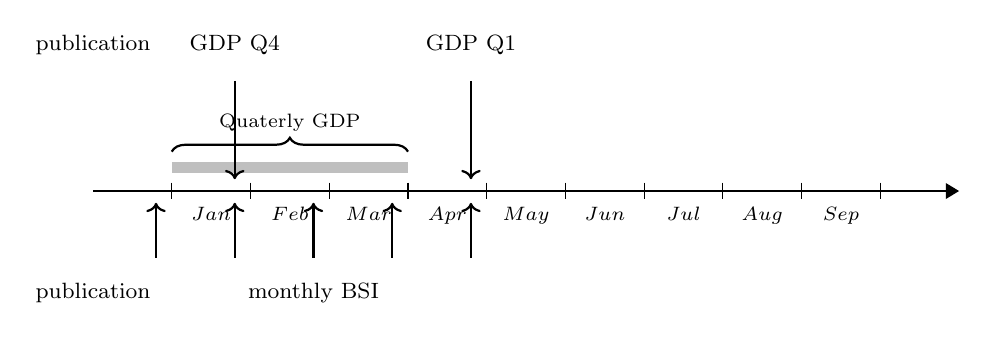
\begin{tikzpicture}  \footnotesize
        % draw horizontal line   
        \draw[thick, -Triangle] (0,0) -- (\ImageWidth,0) node[font=\scriptsize,below left=3pt and -8pt]{ };
        % draw vertical lines
        \foreach \x in {1,...,10}
        \draw (\x cm,3pt) -- (\x cm,-3pt);
        \foreach \x/\descr in {1.5/Jan, 2.5/Feb, 3.5/Mar, 4.5/Apr, 5.5/May, 6.5/Jun, 7.5/Jul, 8.5/Aug,9.5/Sep}
        \node[font=\scriptsize, text height=1.75ex,
        text depth=.5ex] at (\x,-.3) {$\descr$};
        % colored bar up
        \foreach \x/\perccol in
        {1/100,2/75,3/25}
        \draw[lightgray, line width=4pt] 
        (\x,.3) -- +(1,0);
        % braces
        \draw [thick ,decorate,decoration={brace,amplitude=5pt}] (1,0.5)  -- +(3,0) 
               node [black,midway,above=4pt, font=\scriptsize] {Quaterly GDP};
        %\draw [thick,decorate,decoration={brace,amplitude=5pt}] (6,-.9) -- +(-1,0)
        %       node [black,midway,font=\scriptsize, below=4pt] {Publication};
        % time of publication
        \node[align=center] at (0,1.85) {publication};
        \node[align=center] at (1.8,1.85) {GDP Q4};
        \draw [thick,->] (1.8,1.4) -- (1.8,0.15);
        \node[align=center] at (4.8,1.85) {GDP Q1};
        \draw [thick,->] (4.8,1.4) -- (4.8,0.15);
        \node[align=center] at (2.8,-1.3) {monthly BSI};
        \node[align=center] at (0,-1.3) {publication};
        \draw [thick,->] (0.8,-0.85) -- (0.8,-0.15);
        \draw [thick,->] (1.8,-0.85) -- (1.8,-0.15);
        \draw [thick,->] (2.8,-0.85) -- (2.8,-0.15);
        \draw [thick,->] (3.8,-0.85) -- (3.8,-0.15);
        \draw [thick,->] (4.8,-0.85) -- (4.8,-0.15);
    \end{tikzpicture}
    \caption{Timeline of the period and the publication of the business survey indicator (BSI) and the Gross Domestic Product (GDP)}
    \label{fig:timeline}
\end{figure}

Nowcasting became a catch-all word and includes a variety of predictive models as Linear regression, ARIMA models, State-Space models, Mixed-data sampling (MIDAS) regressions, Autoregressive Distributed Lag (ARDL) models  and much more.
Indicators that can be used aside from the business survey are average weekly work hours, factory orders for goods, housing permits and stock prices index of consumer expectations, average weekly claims for unemployment insurance and the interest rate and more.


\subsection{Business Cycles}
\label{sec:Business Cycles}

In 1946, \citeauthor{mitchell_measuring_1946} defined a business cycle as a recursive fluctuations, affecting macroeconomics variables. Since then a lot of variables where used to model business cycles but it's commonly admitted that Growth Domestic Product (GDP) is the most important of them. 
A good measure of the growth of GDP is year on year GDP that is obtained as follow

\begin{eqnarray}
	\mbox{YoY GDP} = \frac{\mbox{GDP}_t - \mbox{GDP}_{t-12}}{\mbox{GDP}_{t-12}}      \label{eq:YoY GDP}
\end{eqnarray}

\autoref{fig:Business Cycle} shows a simplified version of business cycles theory when using as measure GDP or YoY GDP.

\begin{figure}[htp!]
     \centering \footnotesize
    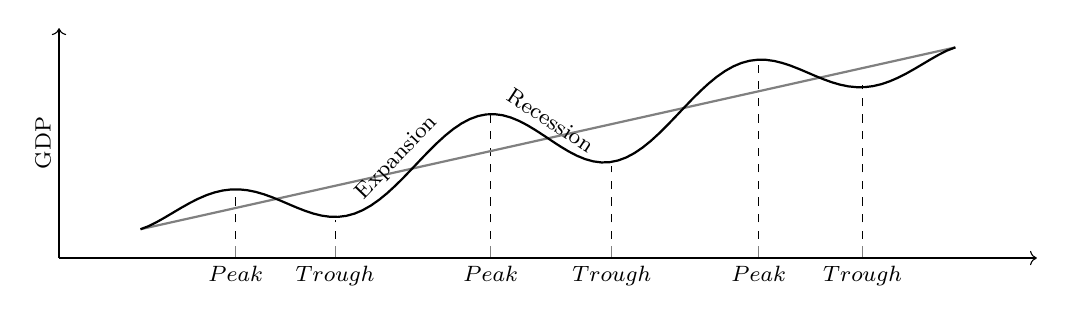
\begin{tikzpicture}  \footnotesize
        \begin{axis}[
            domain=0:6*pi,
            samples=100,
            axis lines*=left, 
            axis line style={->},
            xtick={2.2, 4.5, 8.1, 10.9, 14.3, 16.7}, ytick=\empty,
            xticklabels = {$Peak$, $Trough$, $Peak$, $Trough$, $Peak$, $Trough$},
            width=14cm, height=4.5cm,
        %    xlabel={time}, 
            ylabel={GDP}
        ]       
        \addplot[mark=none, dashed] coordinates {(2.2, -1) (2.2, 4)};
        \addplot[mark=none, dashed] coordinates {(4.5, -1) (4.5, 1)}; 
        \addplot[mark=none, dashed] coordinates {(8.1, -1) (8.1, 12)}; 
        \addplot[mark=none, dashed] coordinates {(10.9, -1) (10.9, 6.6)}; 
        \addplot[mark=none, dashed] coordinates {(14.3, -1) (14.3, 17.5)}; 
        \addplot[mark=none, dashed] coordinates {(16.7, -1) (16.7, 14.9)}; 
        \addplot [thick, gray] {x};
        \addplot [thick, black] {x + 4*sin(deg(x)) * sin(deg(x/6))^0.5}
        %    node [pos=0.1, anchor=south] {Peak}
            node [pos=0.3, anchor=south, sloped] {Expansion}
            node [pos=0.49, anchor=south, sloped] {Recession}
        % Add line to show end of and ... peak and ... line
        ;
        \end{axis}
    \end{tikzpicture}
        
    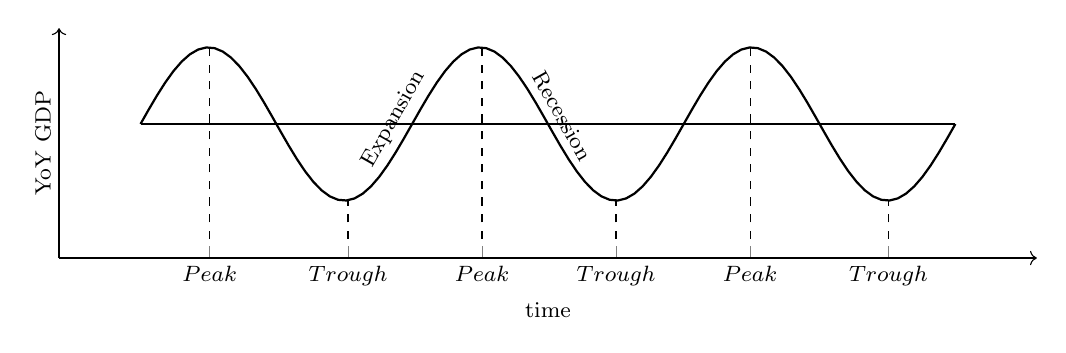
\begin{tikzpicture}  \footnotesize
        \begin{axis}[
            domain=0:6*pi,
            samples=100,
            axis lines*=left, 
            axis line style={->},
            xtick={1.6, 4.8, 7.9, 11, 14.1, 17.3}, ytick=\empty,
            xticklabels = {$Peak$, $Trough$, $Peak$, $Trough$, $Peak$, $Trough$},
            width=14cm, height=4.5cm,
            xlabel={time}, 
            ylabel={YoY GDP}
        ]       
        \addplot [thick, black] {sin(deg(x))}
        %    node [pos=0.1, anchor=south] {Peak}
            node [pos=0.33, anchor=south, sloped] {Expansion}
            node [pos=0.5, anchor=south, sloped] {Recession}
        ;
        \addplot [thick, black] {0};
        \addplot[mark=none, dashed] coordinates {(1.6, -1.5) (1.6, 1)};
        \addplot[mark=none, dashed] coordinates {(4.8, -1.5) (4.8, -1)}; 
        \addplot[mark=none, dashed] coordinates {(7.9, -1.5) (7.9, 1)}; 
        \addplot[mark=none, dashed] coordinates {(11, -1.5) (11,-1)}; 
        \addplot[mark=none, dashed] coordinates {(14.1, -1.5) (14.1, 1)}; 
        \addplot[mark=none, dashed] coordinates {(17.3, -1.5) (17.3, -1)}; 
        \end{axis}
        \end{tikzpicture}
    \caption{The Business Cycle theory of GDP and year on year GDP}
    \label{fig:Business Cycle}
\end{figure}


A very important question considering business cycles is their duration.
\autoref{fig:Business Cycle} can give the false impression that business cycles are all of the same lengths, this is, in real life, not so simple.

Probably the first person to explore the duration of a business cycle was a French statistician,  \cite{juglar_crises_1862}, who set the business cycles to have a duration of 7 to 11 years.
\cite{mitchell_measuring_1946} proposed a minimum duration of 16-22 months and a maximum duration of 100-106 months.
Lot of other propositions where done even though business cycles are rather empirically defined than theory based.
Therefore let put the theory aside and look into real data.
The example of the United States is interesting since the National Bureau of Economic Research (NBER) dated precisely and methodologically the turning points for the American economy. The empirical evidence that comes out of this work, is that the time from one economic peak to the next is on average 5 and a half years for the period 1945-2009.

We can see from \autoref{fig:NBER BS}, which represent the different bottoms and peaks of business cycles identified by the NBER from 1975 to 2009, that there is no symmetry of the business cycles. Some business cycles are very short while others last more than ten years.
We can notice that periods of economic growth, usually last longer than economical decrease.

\begin{figure}[H]
     \centering \footnotesize
    \small
    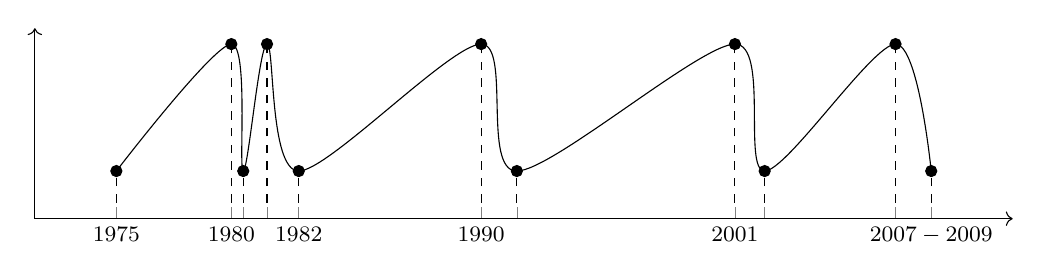
\begin{tikzpicture}  \footnotesize
        \begin{axis}[
            domain=0:6*pi,
            samples=100,
            axis lines*=left, 
            axis line style={->},
            xtick={2103, 2161, 2167, 2179, 2195, 2287, 2305, 2415,2430, 2496, 2514}, ytick=\empty,
            xticklabels = {$1975$, $1980$,  , , $1982$, $1990$, , $2001$, , ,$2007-2009$},
            width=14cm, height=4cm
        %    xlabel={time} 
        %    ylabel={YoY GDP}
        ]       
            \addplot[smooth, mark=*,black] plot coordinates {
            (2103,-1)
            (2161,1)    (2167,-1)
            (2179,1)    (2195,-1)
            (2287,1)    (2305,-1)
            (2415,1)    (2430,-1)
            (2496,1)    (2514,-1)
            };
        \addplot[mark=none, dashed] coordinates {(2103, -1.5) (2103, -1)};
        \addplot[mark=none, dashed] coordinates {(2161, -1.5) (2161, 1)}; 
        \addplot[mark=none, dashed] coordinates {(2167, -1.5) (2167, -1)}; 
        \addplot[mark=none, dashed] coordinates {(2179, -1.5) (2179, 1)}; 
        \addplot[mark=none, dashed] coordinates {(2195, -1.5) (2195,-1)}; 
        \addplot[mark=none, dashed] coordinates {(2287, -1.5) (2287, 1)}; 
        \addplot[mark=none, dashed] coordinates {(2305, -1.5) (2305,-1)}; 
        \addplot[mark=none, dashed] coordinates {(2415, -1.5) (2415, 1)}; 
        \addplot[mark=none, dashed] coordinates {(2430, -1.5) (2430, -1)}; 
        \addplot[mark=none, dashed] coordinates {(2496, -1.5) (2496, 1)}; 
        \addplot[mark=none, dashed] coordinates {(2514, -1.5) (2514, -1)}; 
        \end{axis}
    \end{tikzpicture}
      \caption[Business cycles from 1975 to 2009 of the American Economy according to the NBER]{Business cycles from 1975 to 2009 of the American Economy according to the NBER\footnotemark}
    \label{fig:NBER BS}
\end{figure}

\footnotetext{data available at \url{https://www.nber.org/cycles.html}}

\section{Methodology of the Business Survey}
\label{section:Methodology}

%The latest large improvement of the business survey is explained in detail in \textit{"The National Bank of Belgium’s new business survey indicator"} (\citeauthor{de_greef_national_2009}).

Since 65 years of existence, the business survey was able to evolve without losing in long term comparability.
Three main methodology revisions since the launch of the business survey, in 1983, 1990 and 2009 \cite{de_greef_national_2009}.
The most significant changes brought in 2009 where the number of questions taken into the calculation of the BSI, which was reduced to 3-4 questions, depending on the sector, for more simplicity and accuracy.
Other improvements where the inclusion of the sector of services in the calculation of the global indicator and a new, simple method of smoothing the indicator.

\subsection{Sampling Method}
\label{sec:Recruitment of participants}

The Belgian business survey - as most of the business surveys around the world - has the particularity of not using random sampling. 
The selection of participants is quite complex and a lot of decisions are human, never is a statistical program or a random sampling system used to select new participants.

The selection of new participants is done by waves. When the department responsible for the business survey at the NBB decides that there aren't enough participants in a specific sector anymore, the recruitment of new participants is launched.

To find new respondents, the first step is to decide for an optimal amount of new participants needed, regarding the different stratification of the sector.
Each sector is composed of quite advanced trees of sub-sectors, sub-sub-sectors,  and more. For example, the industry sector is divided into more than 300 sub-sectors / branches over 6 different levels. 

It could be that some subdivision of a certain sector only has 1 or 2 respondents while it accounts for a significant part of the Belgian economy. The Department of the business survey of the NBB will then look into which company, from that specific part of the economy, could be a good fit as new respondent of the business survey, considering its activity, it's size, region, and other characteristics.
As will be seen in \autoref{sec:Weighting procedure} more in detail, companies are weighted by there size (profit, number of employees, ...) and the size of the sector/branch they are part of. That information is crucial for selecting new participants.
The procedure is quite complex and therefore contains a lot of human decisions.
 
Out of this process comes a list of potential new participants. This list is then sent to the Communication Department that makes contact with those potential new participants. 
Not always, but usually, a representative of the National Bank visits the new participant to explain the survey and have a contact.
As a reward for participating in the survey, the companies receive privileged information. Each month they receive access to sub-sector indicators information that aren't publicly distributed. This can give them economical information regarding their specific sector of economic activity.

At the National Bank of Belgium, this procedure is usually referred to as prospecting, rather than selecting or sampling, since it is mostly based on recruiting new companies that will work/collaborate with them. New companies can be included in the survey outside of this procedure but this happens more occasionally.


An important side of the business survey is that people are staying as long as possible in the survey.
From the moment companies are part of the survey, they stay in it until they decide to leave, there are no participants removed from the survey by the National Bank, what can happen is that if participants don't answer for three months, contact will be taken with the company to see if they want to continue to participate.

There are resources put by the National Bank to make sure companies answer to the survey, and stay in it.
This means that some companies are part of the survey for a very long time.
To have an idea, when looking at the survey for the industry and trace respondents back to 30 years ago (1989), it's seen that today, approximately one-third of the respondents were already in the survey in 1988.


From a statistical point of view, it can seem rather problematic to draw general conclusions over a population when not using random sampling.
Without undermining one of the most important pillars of statistics, there are two main reasons why in this case, having a non-random selection of participants is not truly problematic.
The first reason is that the sampling method used is trying to represent as good as possible the population that it is representing. Therefore stratification is used at a quite advanced level as explained before. 
We could call this recruitment method: non-random stratification, as opposed to random stratification. Since it's not using sampling but takes into account the stratification of the population it's studying.
The second reason, the most import one, is that the value of the business survey indicator doesn't have interest on its own. Indeed having a BSI equal to 0.5 or 0.1 doesn't mean much, what's important is the evolution of the indicator. If it was equal to 0.3 last month and this month it's equal to 0.5, it means that the economy is most probably growing and that an increase of GDP over the month can be forecast. On the other hand, if it's now equal to 0.1, it means a decrease in economic confidence among businesses and a deceleration or decline of the economy over the month can be anticipated.



\subsection{Questionnaire}
\label{sec:Questionnaire}

The questionnaire exists in two languages, french and dutch (see Appendix \autopageref{Questionnaire2018}). It can be answered by mail, email, over the phone or by fax.
It is divided into two part:
(1) questions concerning current production and level of activity (\textit{"verloop en beoordeling"}) and
(2) questions concerning predictions, expectation of the level of activity over the next three months ("\textit{vooruitzichten voor de volgende drie maanden}").

The business survey indicator is also called the confidence indicator, since its a measure of how confidence companies are in the Belgian economy.
Almost all the questions have only three possible answers that can be interpreted as a negative, neutral or positive answer.

In this paper, the answers and results of the industry business survey barometer will be used since 1988. Therefore it's very important to see if modifications were applied over time to the questionnaire.
A questionnaire from 1990 can be seen in appendix (see \autopageref{Questionnaire1990}) and can be compared to a more recent version (see appendix \autopageref{Questionnaire2018}).

The layout was modified, and the phrasing of the questions changed over this long period. It was before asked in the first person while it's now phrased in the third person. Aside from those small changes, the survey kept the same questions and order.
It would be interesting to have a closer look at the potential consequences of those changes over time. The layout, the phrasing and the method of answering can potentially influence the answers. Nevertheless, since it's not the subject of this paper, this study will be left for future research.
What can be said, is that the influence of those changes could be limited since the respondents where mostly the same when the changes happened, so the interpretation they made from the questions could have a smaller impact.

The interest of this paper is the industry business survey indicator, which takes four questions into account (questions 18, 27, 32 and 33). The questions are translated into English on \autopageref{Appendix: Question NS975 description} and are renumbered from 1 to 4 for simplicity.
The two first questions relate to the current state of the company while the two others ask the participants there prediction for the next three months.
The first question is about the stock of the company, 
the second question relates to the demand of there product, 
the third questions relate to the company's predictions of need of work forces 
and the last question ask their predictions regarding demand.


\subsection{Weighting Procedure}
\label{sec:Weighting procedure}

The different companies participating in the business survey have all two weights; (1) according to the size of the company and (2) according to the size of the sector branch which the company is part of.
The weight size is calculated based on the profit the company is making, the capital it's owning, the number of employees and other characteristics. 
The calculation is quite complex and is specific to each sector. 
For example, the companies having an industrial activity have a different calculation than a restaurant or a financial services company.

Since the characteristics taken into account during the calculation of the weight of each company aren't fixed, the weight of the companies is corrected periodically. 
Ones the new weight is calculated, the transition between the old and new weight is smoothened over a year. The difference between the new and old weights is divided by 12 and is then adapted each month for a year.

Regarding the globalisation weighting procedure, the National Bank of Belgium developed an elaborate division of the Belgian economic activity. This means that for example, the industry is subdivided into different sub-sectors, that they self contain sub-sectors that contain sub-sectors and so on for a total of six levels. 
Each division has a percentage according to its size in the economy.
To obtain the weight of the lowest globalisation, the weight of each subdivision need to be multiply. 

The procedure of weighting is then as follow

\begin{eqnarray}
    \omega_i = \frac{ \text{weight company $i$} }{ \sum\text{company weights within globalisation} } * \text{globalisation weight} \\ \nonumber
\end{eqnarray}

where $\sum_{i=1}^{n} \omega_i = 1 $. In other words, the specific weight for each company taking the two weighting procedures into account ($\omega_i$), is obtained by dividing its weight coefficient by the total of weight coefficients within the lowest level of globalisation and multiply it with the weight of globalisation it's part of. 


\section{Calculation of the Business Survey Indicator}

This section presents the method of calculation of the business survey indicator.
The calculation in itself is rather standard, but the different ways to write it are important for the interpretation and a better understanding of the indicator and the following chapters.
We first present the calculation taking into account one question unweighted and then weighted. 
The last part will present how different questions are combined together to obtain a business survey indicator.


\subsection{Unweighted Business Survey Indicator}

The calculation of the unweighted indicator for a specific question at a specific time is the mean of the responses and can be written as follow;

\begin{equation}
    \E(X) = \frac{ \sum_{i=1}^n x_i}{n}
\end{equation} 

where 
$x_i$ is the answer of the respondent $i$ and can take value $-1$ (negative answer), $0$ (neutral answer) and $1$ (positive answer). 
$n$ is the number of respondents.

Since $x_i$ can only take three different values, it can be decompose into 

\begin{equation}
    \E(X) = \frac{ \sum_{i=1}^{n_+} x_{+i} + \sum_{i=1}^{n_0} x_{0i} + \sum_{i=1}^{n_-} x_{-i}}{n}
\end{equation} 


where 
$x_{+i}$, $x_{0i}$ and $x_{-i}$ are the positive (+), neutral (N) and negative (-) answers of the respondent $i$.

Since it's known that $\sum_{i=1}^n x_{0i} = 0$, $x_{+i} = 1$ and $x_{-i} = -1$ the equation can be written as follow

\begin{equation}
    \E(X) = \frac{n_+}{n}  - \frac{n_-}{n}
\end{equation} 

Where ${n_+}/{n}$ is the proportion of positive answers and ${n_-}/{n}$ is the proportion of negative answer. The following equation and notation is chosen

\begin{equation}
    \E(X) = \pi_+ - \pi_-  \label{eq: BSI Unweighted}
\end{equation}

where $\pi_+$ and $\pi_-$ are the proportion of respondents answering positive and negative to the specific question.
$\pi$ was chosen as symbol here since it can be interpreted as a probability: if it's assumed that all the respondents have the same probability of giving a certain answer, $\pi$ is the probability that a respondent answers positive ($\pi_+$), negative  ($\pi_-$) or neutral ($\pi_0$) to the question. 


\subsection{Weighted Business Survey Indicator}

As described in \autoref{sec:Weighting procedure}, each respondent has two different weights: one according to its size, one according to the size of the sector it's part of. Those weights are then combined and end up with a specific weight $\omega_i$.
The business survey indicator is then obtained with the following equation 

\begin{equation}
    \E(X) = \sum_{i=1}^n \omega_i x_i  \quad \text{  where  } \sum_{i=1}^n \omega_i =  1
\end{equation} 

$x_i$ is the answer of the respondent $i$ and can take values -1, 0 and 1.
$\omega_i$ is the weight of respondents $i$. 
The weights are standardised so their sum is equal to one.

As for the unweighted indicator, it can be decomposes by the three possible answers with, in this case, their according weights.

\begin{equation}
    \E(X) = \sum_{i=1}^{n_+} \omega_{i} x_{+i} + \sum_{i=1}^{n_0} \omega_{i} x_{0i} + \sum_{i=1}^{n_-} \omega_{i} x_{-i}
 \end{equation}

and again it's known that $\sum_{i=1}^n \omega_{0i} x_{0i} = 0$, $x_{+i} = 1$ and $x_{-i}=-1$ so the equation can be simplified to the following

\begin{equation}
    \E(X) = \sum_{i=1}^{n_+} \omega_{i}  - \sum_{i=1}^{n_-} \omega_{i}
\end{equation}

That will be write as follow

\begin{equation}
    \E(X) = \Omega_+ - \Omega_- \label{eq: BSI Weighted}
\end{equation}

where $\Omega_+$ and $\Omega_-$ are the sum of weights of positive and negative respondents. 
In other words, $\Omega_+$ and $\Omega_-$ are the weighted proportion of respondents answering positive and negative. 

$\Omega$ can also be interpreted in a probabilistic way, as it is the weighted probability that a respondent answers positive ($\Omega_+$), negative ($\Omega_-$) or neutral ($\Omega_0$) assuming all the respondents have the same weighted probability of answering a certain way.
% with $\Omega_+ + \Omega_0 + \Omega_- =1$. Here we speak of weighted proportions/probabilities.

From \autoref{eq: BSI Unweighted} and \ref{eq: BSI Weighted} it can be seen that the weighted and unweighted indicators are bounded between -1 and 1. In the two cases, the indicator is the smallest if all respondents have a negative answer, and is the largest when every answer is positive.

\subsection{Take Different Questions Into Account}

The previous calculations were specific to one question. The published indicators are usually taking different survey questions into account. For example, the industry indicator, that will be at interest, is composed of four questions:

\begin{equation}
    \mbox{Industry BSI}\ = \frac{\E(X_{Q1}) + \E(X_{Q2}) + \E(X_{Q3}) + \E(X_{Q4})}{4}
\end{equation}

where 
$\E(X_{Q1})$, $\E(X_{Q2})$, $\E(X_{Q3})$ and $\E(X_{Q4})$ are the different averages for question 1, 2, 3 and 4 (see \autopageref{Appendix: Question NS975 description}). The averages can be weighted or unweighted.

The equation can also be written as follow for the unweighted indicator\footnote{Assuming the respondents that answered, answered to all the questions.}

\begin{equation}
    \mbox{Unweighted Industry BSI}\ = \frac{\sum^n_{i=1}(x_{iQ1} + x_{iQ2} + x_{iQ3} + x_{iQ4})}{4n} 
\end{equation} 

and as follow for the weighted indicator\footnote{Assuming the respondents that answered, answered to all the questions and that the weighting ($\omega_i$) is the same across all the questions.}

\begin{equation}
    \mbox{Weighted Industry BSI}\ = \frac{\sum^n_{i=1} \omega_i (x_{iQ1} + x_{iQ2} + x_{iQ3} + x_{iQ4})}{4} 
\end{equation} 

In other words, the industry BSI is the weighted or unweighted mean of responses of all the respondents.

Another way to write the unweighted business survey indicator is as follow

\begin{eqnarray}
    \mbox{Unweighted industry BSI}\ &=& \frac{1}{4} \big( \pi_{Q1,+} + \pi_{Q2,+} + \pi_{Q3,+} + \pi_{Q4,+} \nonumber \\
    && - \pi_{Q1,-} - \pi_{Q2,-} - \pi_{Q3,-} - \pi_{Q4,-} \big)
\end{eqnarray}

and regarding the weighted indicator, it can be written as

\begin{eqnarray}
    \mbox{ Weighted Industry BSI}\ &=& \frac{1}{4} \big( \Omega_{Q1,+} + \Omega_{Q2,+} + \Omega_{Q3,+} + \Omega_{Q4,+} \nonumber \\
    && - \Omega_{Q1,-} - \Omega_{Q2,-} - \Omega_{Q3,-} - \Omega_{Q4,-} \big) 
\end{eqnarray}

The weighted or unweighted industry BSI are here equal to to difference between the positive proportions and the negative proportions of responses.


The previous equations can easily be generalised to all combinations of answers in the calculation of indicators.
The general formulas for the unweighted business survey indicator when taking several questions into account can be written as follow

\begin{eqnarray}
    \mbox{Unweighted BSI} &=& \frac{\E(X_{Q1}) + \E(X_{Q2}) + \ldots + \E(X_{Qq})}{q} \\
    &=& \frac{\sum^n_{i=1}( x_{iQ1} + x_{iQ2} + \ldots + x_{iQq})}{nq} \\
    &=& \frac{1}{q} \big( \pi_{Q1,+} +  \pi_{Q2,+} + \ldots +  \pi_{Qq,+}  -  \pi_{Q1,-} -  \pi_{Q2,-} - \ldots - \pi_{Qq,-} \big) \nonumber\\
\end{eqnarray}
Where $q$ is the number of questions taken into account for the calculation of the indicator.

The formulas for the weighted business survey indicator when taking several questions into account can be written as follow

\begin{eqnarray}
    \mbox{ Weighted BSI} &=& \frac{\E(X_{Q1}) + \E(X_{Q2}) + \ldots + \E(X_{Qq})}{q} \\
    &=& \frac{\sum^n_{i=1} \omega_i \left( x_{iQ1} + x_{iQ2} +\ldots + x_{iQq} \right)}{q} \\    
    &=& \frac{1}{q} \big( \Omega_{Q1,+} + \Omega_{Q2,+} + \ldots + \Omega_{Qq,+} - \Omega_{Q1,-} - \Omega_{Q2,-} - \ldots - \Omega_{Qq,-} \big) \nonumber\\
\end{eqnarray}





\chapter{The Variance of the Business Survey Indicator}

The variance is, with the mean, one of the first tool for statisticians to study a certain variable. 
Next, to the mean, that is the average value of a certain variable, the variance is the measure of the dispersion. 
In the context of the business survey, the variance can be seen as "how much companies (dis)agree on the present state of the Belgian economy", a piece of important information that can be extracted from the survey.

% A small comment can be written regarding the difference between the variance and sampling error. The idea here is not the study accuracy or ... but rather to find new information hidden in the survey.

This chapter will present the calculation of the variance of the unweighted and weighted indicator for one question of the business survey. It will then be looked into its properties and specificities.
The last section will present the method of calculation when different questions are taken into account.

\section{Variance of the Unweighted Business Survey Indicator}

\nocite{alcaniz_calculation_2006}

The formula of the variance can be written as 
\begin{eqnarray}
         \Var(X) &=& E \left[ \left(X-\E(X) \right)^2 \right] =  E\left( X^2\right) - E\left( X\right)^2 \\ \nonumber
\end{eqnarray}

The variance of one question of the unweighted business survey indicator be decomposed and developed as follow,

\begin{eqnarray}
\Var(X) &=&  E\left( X^2\right) - E\left( X\right)^2 \nonumber \\ \nonumber \\
    &=&  \frac{\sum_{i=1}^{n_+} x_{+i}^2  +  \sum_{i=1}^{n_0} x_{0i}^2 + \sum_{i=1}^{n_-} x_{-i}^2}{n}  - \E(X)^2 \\ \nonumber
\end{eqnarray}


Since the positive answers take value 1 and negative answers value -1, there square are equal to 1 ($x_{+i}^2 = x_{+i} = 1$ and $x_{-i}^2 = |x_{-i}| = 1$). 
On the other hand, the neutral answers have value 0, and can therefore be taken out of the equation.

The equation can further be simplified to

\begin{eqnarray}
    \Var(X) &=&  \frac{n_+}{n}  +  \frac{n_-}{n}  - \E(X)^2 \\
    &=& \pi_+ + \pi_- - E ( X )^2 \label{var1} \\ \nonumber
\end{eqnarray}

Where $\pi_+$ and $\pi_-$ are the proportions of positive and negative answers.

In other words, the variance of the BSI is equal to the sum of the proportion of positive and negative answers, minus the squared indicator.

Knowing $\E(X)=\pi_+ - \pi_-$, and $\pi_+ + \pi_- = 1 - \pi_0$ (from $\pi_+ + \pi_0 + \pi_- = 1$),
it's possible to write the variance in several different ways;

%We can also replace $\E(X)$  by $\pi_+ - \pi_-$, and/or $\pi_+ + \pi_-$ by $ 1 - \pi_0$ (since $\pi_+ \pi_0 + \pi_- = 1$). Which means that we have several different ways to write the previous equation;

\begin{eqnarray}
\Var(X) &=& \pi_+ + \pi_- - E ( X )^2  \nonumber \\
        &=& \pi_+ + \pi_- - ( \pi_+ - \pi_- )^2 \label{eq:var2} \\
        &=& 1 - \pi_0 - \E(X)^2 \label{eq:var3}
\end{eqnarray}




\section{Variance of the Weighted Business Survey Indicator}

We can now do the same for the weighted indicator. The equation is very similar to the variance of the unweighted variance

\begin{eqnarray}
\Var(X) &=&  E\left( X^2\right) - E\left( X\right)^2 \nonumber \\ \nonumber \\
    &=& \sum_{i=1}^{n_+} \omega_i x_{+i}^2 + \sum_{i=1}^{n_0} \omega_i x_{0i}^2  + \sum_{i=1}^{n_-} \omega_i x_{-i}^2 - \E(X)^2 \\
    &=& \sum_{i=1}^{n_+} \omega_i + \sum_{i=1}^{n_-} \omega_i - \E(X)^2 \nonumber \\
\end{eqnarray}

As done for the indicator, the equation is further developed by taking into account weighted proportion and write the equation the same way as for the unweighted variance. 
Again the variance can be written in different ways

\begin{eqnarray}
\Var(X) &=& \Omega_+ + \Omega_- - E ( X )^2 \\
	&=& \Omega_+ + \Omega_- - ( \Omega_+ - \Omega_- )^2 \\
    &=& 1 - \Omega_{0} - \E(X)^2 \label{eq:var3 weighted}
\end{eqnarray}


\section{Properties}
    \label{sec:properties variance}

\begin{figure}[hbt!]
     \centering \footnotesize
    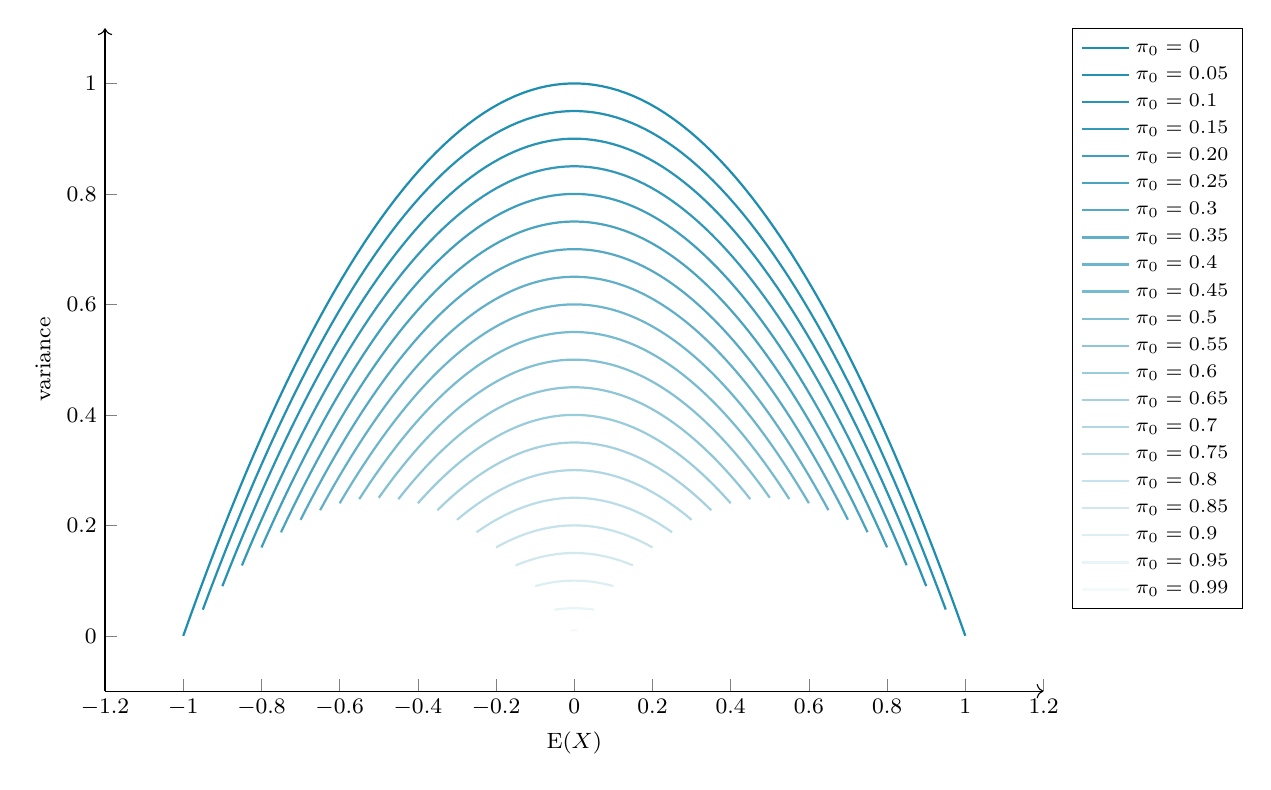
\begin{tikzpicture}  \footnotesize
    \tikzset{
      legendmatrix/.style={% style for legends
        draw,% draw a border for the legend
        outer sep=.3333em,% additional space to the axis label
        nodes={rotate=90,anchor=base west,outer sep=0pt},% rotate the nodes inside the matrix
        /pgfplots/every crossref picture/.append style={yshift=.75ex}% rotate the legend images
      }
    }
    \begin{axis}[
        domain=-1:1,
        samples=100,
        axis lines*=left, 
        axis line style={->},
        width=13.5cm, height=10cm,
        xlabel={$\E(X)$}, ylabel={variance},
    legend pos= outer north east, legend cell align=left,
     legend style={font=\scriptsize}
     ]       
    \addplot [thick, bluetitle!100, domain = -1:1] {1 - x^2};
    \addplot [thick, bluetitle!97, domain = -0.95:0.95] {1 - 0.05 - x^2};
    \addplot [thick, bluetitle!95, domain = -0.9:0.9] {1 - 0.1 - x^2};
    \addplot [thick, bluetitle!90, domain = -0.85:0.85] {1 - 0.15 - x^2};
    \addplot [thick, bluetitle!85, domain = -0.8:0.8] {1 - 0.2 - x^2};
    \addplot [thick, bluetitle!80, domain = -0.75:0.75] {1 - 0.25 - x^2};
    \addplot [thick, bluetitle!75, domain = -0.7:0.7] {1 - 0.3 - x^2};
    \addplot [thick, bluetitle!70, domain = -0.65:0.65] {1 - 0.35 - x^2};
    \addplot [thick, bluetitle!65, domain = -0.6:0.6] {1 - 0.4 - x^2};
    \addplot [thick, bluetitle!60, domain = -0.55:0.55] {1 - 0.45 - x^2};
    \addplot [thick, bluetitle!55, domain = -0.5:0.5] {1 - 0.5 - x^2};
    \addplot [thick, bluetitle!50, domain = -0.45:0.45] {1 - 0.55 - x^2};
    \addplot [thick, bluetitle!45, domain = -0.4:0.4] {1 - 0.6 - x^2};
    \addplot [thick, bluetitle!40, domain = -0.35:0.35] {1 - 0.65 - x^2};
    \addplot [thick, bluetitle!35, domain = -0.3:0.3] {1 - 0.7 - x^2};
    \addplot [thick, bluetitle!30, domain = -0.25:0.25] {1 - 0.75 - x^2};
    \addplot [thick, bluetitle!25, domain = -0.2:0.2] {1 - 0.8 - x^2};
    \addplot [thick, bluetitle!20, domain = -0.15:0.15] {1 - 0.85 - x^2};
    \addplot [thick, bluetitle!15, domain = -0.1:0.1] {1 - 0.9 - x^2};
    \addplot [thick, bluetitle!10, domain = -0.05:0.05] {1 - 0.95 - x^2};
    \addplot [thick, bluetitle!05, domain = -0.01:0.01] {1 - 0.99 - x^2};
 %    \addplot [thick, black, domain = -1:0] { - ((x+0.5)^2) + 0.25};
 %    \addplot [thick, black, domain = 0:1] { - ((x-0.5)^2) + 0.25};
%     \addplot [thick, black, domain = -1:0] {-x-x^2};
%     \addplot [thick, black, domain = 0:1] {x-x^2};
%     \addplot [thick, black, domain = -1:1] {(x^2)*(-y)-(y^2)/2 + y};    
    \addlegendentry{$\pi_0 = 0$}
    \addlegendentry{$\pi_0 = 0.05$}
    \addlegendentry{$\pi_0 = 0.1$}
    \addlegendentry{$\pi_0 = 0.15$}
    \addlegendentry{$\pi_0 = 0.20$}
    \addlegendentry{$\pi_0 = 0.25$}
    \addlegendentry{$\pi_0 = 0.3$}
    \addlegendentry{$\pi_0 = 0.35$}
    \addlegendentry{$\pi_0 = 0.4$}
    \addlegendentry{$\pi_0 = 0.45$}
    \addlegendentry{$\pi_0 = 0.5$}
    \addlegendentry{$\pi_0 = 0.55$}
    \addlegendentry{$\pi_0 = 0.6$}
    \addlegendentry{$\pi_0 = 0.65$}
    \addlegendentry{$\pi_0 = 0.7$}
    \addlegendentry{$\pi_0 = 0.75$}
    \addlegendentry{$\pi_0 = 0.8$}
    \addlegendentry{$\pi_0 = 0.85$}
    \addlegendentry{$\pi_0 = 0.9$}
    \addlegendentry{$\pi_0 = 0.95$}
    \addlegendentry{$\pi_0 = 0.99$}
    \end{axis}
    \end{tikzpicture}
    \caption{Plot of the possible values of the indicator (X axis) and variance (Y axis) for different values of $\pi_0$ }
    \label{fig:var properties}
\end{figure}


Based on the previous development of the equation of the variance of the indicator, some observations can be done.

First of all, the variance is bounded between 0 and 1. 
A variance can't be negative since it's a sum of squares, so the lower bound shouldn't surprise anyone. On the other hand, the upper bound is more unusual. 
An interesting approach is to take  \autoref{eq:var3} and see that $\pi_0$ and $\E(X)^2$ can only take positive values since $\pi_0$ is a proportion and $\E(X)^2$ is squared. 
Both variables have a minus sign in the equation, so the highest results are obtained when both variables are equal to zero.
In other words, the highest variance is obtained when no respondent answers "neutral" and the BSI is equal to 0. 
This happens when there are as many negative as positive answers (50-50).
This corresponds to the interpretation described before since it's the situation with the most disagreement among respondents.
In the other hand, if all participants answer the same ("negative", "neutral" or "positive"), the variance is equal to zero.
It corresponds to the situation where the agreement among respondents is the highest.

Another approach to better understand the variance of the business survey barometer, is to plot the different possible values of $\Var(X)$, $\pi_0$ and $\E(X)$ from \autoref{eq:var3} or \autoref{eq:var3 weighted}. The results can be seen in \autoref{fig:var properties}.
It's interesting to see from the plot that each $\E(X)$ can only have a certain amount of possible variance, in other words, there is a specific upper and lower bound for each indicator. For example, an indicator of 0.5 can only have a variance between 0.25 and 0.75.
It's also interesting to notice that to know that with two of the three variables ($\Var(X)$, $\pi_0$ and $\E(X)$), it's very easy to calculate the third. This means that the three variables are related.

\section{Take Different Questions Into Account}

As already seen, the published indicator takes different questions into account. 
The combination of the variance of different questions is slightly more complex than the combination of different indicators since the questions are correlated, which means that covariance has to be taken into account.

The formula to combine different variances is the following

\begin{eqnarray}
\Var \left(\sum_{i=1}^{q} X_{i}\right) = \sum_{i=1}^{q} \sum_{j=1}^{q} \Cov\left(X_{i}, X_{j}\right)
= \sum_{i=1}^{q} \Var\left(X_{i}\right)+2 \sum_{1 \leq i<j \leq q} \Cov\left(X_{i}, X_{j}\right) \label{eq:sum of variances} \\ \nonumber
\end{eqnarray} 

In the case of combining the variances of the four different questions of the industry business survey, the following equation applies

\begin{eqnarray}
    \Var \left( \text{Industry BSI} \right) 
    &=& \frac{1}{16} \Big[ \Var(X_{Q1}) + \Var(X_{Q2}) + \Var(X_{Q3}) + \Var(X_{Q4}) \nonumber \\
    && + 2 \Cov (X_{Q1},X_{Q2}) + 2 \Cov (X_{Q1},X_{Q3}) + 2 \Cov (X_{Q1},X_{Q4}) \nonumber \\
    &&  + 2 \Cov (X_{Q2},X_{Q3}) + 2 \Cov (X_{Q2},X_{Q4}) + 2 \Cov (X_{Q3},X_{Q4}) \Big] \nonumber \\
\end{eqnarray}

The complexity of the formula encourages to rather calculate the indicator (taking all the questions into account), and then calculate the variance of that indicator, that can be written as follow for the unweighted BSI

\begin{eqnarray}
         \Var(\text{BSI}) &=& E \left[ \left(\text{BSI}-\E(\text{BSI}) \right)^2 \right] =  \E \left( \text{BSI}^2\right) - \E \left( \text{BSI}\right)^2 \\ 
         &=&  \frac{\sum^n_{i=1}[(x_{iQ1} + x_{iQ2} + x_{iQ3} + x_{iQ4})/4]^2}{n} - \E (\BSI)^2 \\
        &=&  \frac{\sum^n_{i=1}(x_{iQ1} + x_{iQ2} + x_{iQ3} + x_{iQ4})^2}{16n} - \E (\BSI)^2 \\
        &=& \frac{1}{16} \left( \pi_{Q1,+} + \pi_{Q1,-} + \pi_{Q2,+} + \pi_{Q2,-} + \pi_{Q3,+} + \pi_{Q3,-} + \pi_{Q4,+} + \pi_{Q4,-} \right) - \E (\BSI)^2 \nonumber \\ 
\end{eqnarray}

and for the weighted BSI can be written as follow

\begin{eqnarray}
         \Var(\text{BSI}) &=& E \left[ \left(\text{BSI}-\E(\text{BSI}) \right)^2 \right] =  \E \left( \text{BSI}^2\right) - \E \left( \text{BSI}\right)^2 \\ 
         &=&  \sum^n_{i=1} \left[\omega_i (x_{iQ1} + x_{iQ2} + x_{iQ3} + x_{iQ4})/4 \right]^2 - \E (\BSI)^2 \\
         &=& \frac{1}{16} \left( \Omega_{Q1,+} + \Omega_{Q1,-} + \Omega_{Q2,+} + \Omega_{Q2,-} + \Omega_{Q3,+} + \Omega_{Q3,-} + \Omega_{Q4,+} + \Omega_{Q4,-} \right) - \E (\BSI)^2 \nonumber \\ 
\end{eqnarray}

where $\BSI = \left(x_{i Q1} + x_{i Q2} + \ldots + x_{i Qq} \right) / q $ in the case of the unweighted indicator and $\BSI = \omega \left(x_{i Q1} + x_{i Q2} + \ldots + x_{i Qq} \right) / q $



The generalisation of the previous equation - when taking $q$ questions into account - can be written as follow for the variance of the unweighted indicator

\begin{eqnarray}
         \Var(\text{BSI}) &=& E \left[ \left(\text{BSI}-\E(\text{BSI}) \right)^2 \right] =  \E \left( \text{BSI}^2\right) - \E \left( \text{BSI}\right)^2 \\ 
         &=&  \frac{\sum^n_{i=1}[(x_{iQ1} + x_{iQ2} + \ldots + x_{iQq})/q]^2}{n} - \E (\BSI)^2 \\
        &=&  \frac{\sum^n_{i=1}(x_{iQ1} + x_{iQ2} + \ldots + x_{iQq})^2}{q^2 n} - \E (\BSI)^2 \\
        &=& \frac{1}{q^2} \left( \pi_{Q1,+} + \pi_{Q1,-} + \pi_{Q2,+} + \pi_{Q2,-} + \ldots + \pi_{Qq,+} + \pi_{Qq,-} \right) - \E (\BSI)^2 \nonumber \\ 
\end{eqnarray}

and as follow for the weighted BSI

\begin{eqnarray}
         \Var(\text{BSI}) &=& E \left[ \left(\text{BSI}-\E(\text{BSI}) \right)^2 \right] =  \E \left( \text{BSI}^2\right) - \E \left( \text{BSI}\right)^2 \\ 
         &=&  \sum^n_{i=1} \left[\omega_i (x_{iQ1} + x_{iQ2} + \ldots + x_{iQq})/q \right]^2 - \E (\BSI)^2 \\
         &=& \frac{1}{q^2} \left( \Omega_{Q1,+} + \Omega_{Q1,-} + \Omega_{Q2,+} + \Omega_{Q2,-} + \ldots + \Omega_{Qq,+} + \Omega_{Qq,-} \right) - \E (\BSI)^2 \nonumber \\ 
\end{eqnarray}




\chapter{The Evolution of Individual Responses}

In the same logic as for the variance, a proposition is done in this chapter of a method to extract more information out of the business survey. 
As explained in the chapter two - that presented the business survey - the business survey is answered by the same companies over time. Some new participants join and some companies leaving the survey, but the survey can be referred to and treated as a panel survey.

Is it possible to have more information by taking the evolution of the individual respondents into account? 
This chapter will address this question by applying a method proposed by \cite{caron_estimation_1996} that, by taking all the individual evolution of responses into account, offers a method to calculate an indicator that will be referred to as the indicator of the evolution of individual responses (EIR).

% We will here describe and develop this indicator, that we will call Evolution of individual Responses (EIR).
% It can be understood as the indicator of the changes in individual answers between t-1 and t.

When only one period is taken into account, there are three possible answers; "negative", "neutral" and "positive".
When two periods are taken into account - a month (t) and the previous one (t-1) for example - there are nine possible situations as represented in \autoref{tab:EIR explanation}. 


\begin{table}[htp!]
    \caption{Possible observations when taking $t$ and $t-1$ into account}
    \label{tab:EIR explanation}
     \centering \footnotesize
    \begin{tabular}{r | r | c c c | }
    \multicolumn{1}{r}{} & \multicolumn{1}{r}{} &    \multicolumn{3}{c}{$t$} \\ \cline{3-5}
    \multicolumn{1}{r}{} &         & \textbf{$x_{i-}$} & \textbf{$x_{i0}$} & \textbf{$x_{i+}$} \\ \cline{2-5}
          &    \textbf{$x_{i-}$} & $z_{i--}$    & $z_{i-0}$    & $z_{i-+}$ \\ 
    $t-1$ & \textbf{$x_{i0}$}  & $z_{i0-}$    & $z_{i00}$    & $z_{i0+}$ \\
          &    \textbf{$x_{i+}$} & $z_{i+-}$    & $z_{i+0}$    & $z_{i++}$ \\ \cline{2-5}
    \end{tabular}
\end{table}

The same as for the business survey indicator, the evolution of individual responses take different values. In the case of the BSI, $x_i$ can take value -1, 0 and 1. In the case of the EIR, $z_i$ can take values -2, -1, 0, 1 and 2.

The EIR defers also from the BSI in the sense that it's a measure of change, so if the answer of a certain respondent is the same at a certain time and the previous answer, $z_i=0$. 
% What's measured here is the difference in the answer.
On the other hand, if a certain participant changes his answer for a more positive answer it will take value 1, except if it's a radical change from a "negative" to a "positive" answer, then it will take value 2.
Same the other way around, if it decreases it will take value -1, except for a radical change from "positive" to "negative".
We will here use $z$ rather than $x$ to make a clear distinction between the BSI and the EIR.

The calculation of $z_i$ is the difference of $x_i$ at t-1 and $x_i$ at t

\begin{equation}
    z_i = x_{i,t-1} - x_{i,t}
\end{equation}

the different possible values of $z_i$ can be seen in \autoref{tab:values EIR}. 

\begin{table}[htp!]
    \caption{Values of the different observations of $z_i$}
    \label{tab:values EIR}
    \centering \footnotesize
    \begin{tabular}{r | r | c c c | }
    \multicolumn{1}{r}{} & \multicolumn{1}{r}{} &    \multicolumn{3}{c}{$t$} \\ \cline{3-5}
    \multicolumn{1}{r}{} &         & \textbf{$x_{i-}$} & \textbf{$x_{i0}$} & \textbf{$x_{i+}$} \\ \cline{2-5}
           &    \textbf{$x_{i-}$} & $z_{i--}=0$    & $z_{i-0}=1$    & $z_{i-+}=2$ \\ 
    $t-1$ & \textbf{$x_{i0}$}  & $z_{i0-}=-1$    & $z_{i00}=0$    & $z_{i0+}=1$    \\
            & \textbf{$x_{i+}$}& $z_{i+-}=-2$    & $z_{i+0}=-1$    & $z_{i++}=0$ \\ \cline{2-5}
\end{tabular}
\end{table}


The limitation of this indicator is that the previous answer is determinant of the possible results of the indicator. 
If the previous response was neutral (0), then it's possible to influence the EIR in a positive or negative way. 
On the other hand if the previous answer was negative or positive, it can only influence the EIR in the opposite way.

For those reasons, the EIR should be complementary to the BSI rather than replacing it or else.



\section{Indicator of the Unweighted Evolution of Individual Responses}

% \begin{equation}
%    \pi_{++} + \pi_{+0} + \pi_{+-} + \pi_{0+} + \pi_{00} + \pi_{0-} + \pi_{-+} + \pi_{-0} + \pi_{--} = 1
% \end{equation}

The indicator of the evolution of the individual responses can be obtained by taking the mean of the values, as defined in \autoref{tab:values EIR}, the formula is then

\begin{eqnarray}
    \E(Z) &=&  \frac{ \sum_{i=1}^n z_i}{n} \\ \nonumber \\
        &=&  \frac{ \sum_{i=1}^{n_{--}} z_{--i}}{n} 
     +  \frac{\sum_{i=1}^{n_{-0}} z_{-0i} }{n} 
    +  \frac{\sum_{i=1}^{n_{-+}} z_{-+i}}{n} 
    +  \frac{\sum_{i=1}^{n_{0-}} z_{0-i} }{n} 
    +  \frac{\sum_{i=1}^{n_{00}} z_{00i} }{n}  \nonumber \\ \nonumber \\
    &&  +  \frac{\sum_{i=1}^{n_{0+}} z_{0+i}}{n} 
    +  \frac{\sum_{i=1}^{n_{+-}} z_{+-i} }{n} 
    +  \frac{\sum_{i=1}^{n_{+0}} z_{+0i} }{n} 
    +  \frac{\sum_{i=1}^{n_{++}} z_{++i}}{n} 
\end{eqnarray}

The formula can further be simplified since $z_{--} = z_{00} = z_{++} = 0$ and the other values of $z_i$'s are also known

\begin{eqnarray}
    \E(Z) &=&  
      \frac{\sum_{i=1}^{n_{-0}} z_{-0i} }{n} 
    +  \frac{\sum_{i=1}^{n_{-+}} z_{-+i}}{n} 
    +  \frac{\sum_{i=1}^{n_{0-}} z_{0-i} }{n} 
    +  \frac{\sum_{i=1}^{n_{0+}} z_{0+i}}{n}  \nonumber \\ \nonumber \\
&&  +  \frac{\sum_{i=1}^{n_{+-}} z_{+-i} }{n} 
    +  \frac{\sum_{i=1}^{n_{+0}} z_{+0i} }{n}  \\ \nonumber \\
    &=&  
         \frac{n_{-0}}{n} 
    +   \frac{2n_{-+}}{n} 
    -    \frac{n_{0-}}{n} 
    +    \frac{n_{0+}}{n}  
    -   \frac{2n_{+-}}{n} 
    -    \frac{n_{+0}}{n} 
\end{eqnarray}




As for the indicator, it's possible here to have a formula with proportions.

% The EIR can now be calculated with the following expression after taking out $\pi_{--}$, $\pi_{00}$ and $\pi_{++}$ (since $z_{--} = z_{00} = z_{++} = 0$).

\begin{equation}
    \E(Z) = \pi_{0+} + \pi_{-0} - \pi_{+0} - \pi_{0-} +2\pi_{-+} -2\pi_{+-} \label{eq:unweighted proprotion EIR}
\end{equation}

where $\pi$ is the proportion/probability of respondent answering negative(-), neutral (0) and positive (+) at $t-1$ and $t$. 

The evolution of individual responses is equal to the difference between the proportion of respondents becoming more positive and the proportion of respondents becoming more negative. Where radical changes count double.

The EIR can take values between -2 and 2.

% \autoref{eq:unweighted proprotion EIR} shows that 


\section{Indicator of the Weighted Evolution of Individual Responses}

As for the business survey indicator, the evolution of individual responses can also be weighted. The calculation is very similar.

\begin{eqnarray}
    \E(Z) &=&  \sum_{i=1}^n \omega_i z_i \\ \nonumber \\
        &=& \sum_{i=1}^{n_{--}} \omega_i z_{--i} 
     + \sum_{i=1}^{n_{-0}} \omega_i z_{-0i}  
    + \sum_{i=1}^{n_{-+}} \omega_i z_{-+i} 
    + \sum_{i=1}^{n_{0-}} \omega_i z_{0-i}  
    + \sum_{i=1}^{n_{00}} \omega_i z_{00i}   \nonumber  \\
    &&  + \sum_{i=1}^{n_{0+}} \omega_i z_{0+i} 
    + \sum_{i=1}^{n_{+-}} \omega_i z_{+-i} 
    + \sum_{i=1}^{n_{+0}} \omega_i z_{+0i} 
    + \sum_{i=1}^{n_{+-}} \omega_i z_{++i} \\
&=&  \sum_{i=1}^{n_{-0}} \omega_i  
    + 2 \sum_{i=1}^{n_{-+}} \omega_i  
    - \sum_{i=1}^{n_{0-}} \omega_i         
    + \sum_{i=1}^{n_{0+}} \omega_i  
    - 2 \sum_{i=1}^{n_{+-}} \omega_i 
    - \sum_{i=1}^{n_{+0}} - \omega_i  
\end{eqnarray}

The weighted EIR can, as for the unweighted EIR now be calculated with the following expression 

\begin{equation}
    \E(Z) = \Omega_{0+} + \Omega_{-0} - \Omega_{+0} - \Omega_{0-} +2\Omega_{-+} -2\Omega_{+-} \label{eq:weighted proprotion EIR}
\end{equation}

where $\Omega$'s are the different sum of weights, or in other words, weighted proportions.

The formula is very similar to the unweighted and can be interpreted the same way.


\section{Generalisation for Different Period Lags}

Changes in the economy are usually taking several months to influence all the companies. There can be some lag of effects on for example larger companies, of a very specific sector.
The idea of only taking a certain month and the previous month can seem non-sufficient, it's relevant to take a larger period into account. 

Different methods were explored to take more than two periods into account, but it was found to be flawed and very complex to interpret.
We rather propose here a simple generalisation; use t-n rather than t-1. 
The answer at t-n is compared with the answer at time t, without taking the between answers into account.

The calculation is then the same for the unweighted as \autoref{eq:unweighted proprotion EIR} and for the weighted as \autoref{eq:weighted proprotion EIR} except $t-1$ is replaced by $t-n$, the two periods taken into account are the actual month and the n\textsuperscript{th} previous month.


\section{Take Different Questions Into Account}

The generalisation, when taking different question into account in order to obtain an indicator, can be written with the following formula \footnote{Assuming the respondents who participated, answered to all the questions}

\begin{equation}
    \mbox{Industry EIR}\ = \frac{\sum_{i=1}^n \left(z_{i Q1} + z_{i Q2} + \ldots + z_{i Qq} \right)}{qn}
\end{equation}


In the case of the unweighted evolution of individual responses, the formula can be written as follow

\begin{eqnarray}
\mbox{Unweighted EIR}\ &=& \frac{\sum_{i=1}^n \left(z_{i Q1} + z_{i Q2} + \ldots + z_{i Qq} \right)}{qn} \nonumber \\
&=&    \pi_{Q1,0+} + \pi_{Q1,-0} - \pi_{Q1,+0} - \pi_{Q1,0-} +2 \pi_{Q1,-+} -2\pi_{Q1,+-} \nonumber \\
&&    + \pi_{Q2,0+} + \pi_{Q2,-0} - \pi_{Q2,+0} - \pi_{Q2,0-} +2 \pi_{Q2,-+} -2\pi_{Q2,+-} \nonumber \\
&&	 + \ldots \nonumber \\
&&   + \pi_{Qq,0+} + \pi_{Qq,-0} - \pi_{Qq,+0} - \pi_{Qq,0-} +2 \pi_{Qq,-+} -2\pi_{Qq,+-} \nonumber \\
\end{eqnarray}

and the weighted formula of the EIR when taking different question into account can be written as

\begin{eqnarray}
    \mbox{Weighted EIR}\ &=& \frac{ \sum_{i=1}^n \omega_i \left(z_{i Q1,} + z_{i Q2} + \ldots + z_{i Qq} \right)}{q} \nonumber \\
&=&    \Omega_{Q1,0+} + \Omega_{Q1,-0} - \Omega_{Q1,+0} - \Omega_{Q1,0-} +2 \Omega_{Q1,-+} -2\Omega_{Q1,+-} \nonumber \\
&&    + \Omega_{Q2,0+} + \Omega_{Q2,-0} - \Omega_{Q2,+0} - \Omega_{Q2,0-} +2 \Omega_{Q2,-+} -2\Omega_{Q2,+-} \nonumber \\
&&	 + \ldots \nonumber \\
&&   + \Omega_{Qq,0+} + \Omega_{Qq,-0} - \Omega_{Qq,+0} - \Omega_{Qq,0-} +2 \Omega_{Qq,-+} -2\Omega_{Qq,+-} \nonumber \\
\end{eqnarray}




\chapter{The Variance of the Evolution of Individual Responses} \label{Chapter:Var Z}

The evolution of individual responses has a variance that has some  interesting interpretation.
While the EIR is a measure of the direction companies change their answer(s), the variance of the EIR can be understood as the measure of changes in answers.
From there, the variance of the EIR can be seen as the volatility of the indicator, in the sense that the variance of the EIR accounts for the dispersion of the difference in answers over two periods.

While the variance of the business survey indicator is the measure of disagreement among respondents, the variance of the evolution of individual responses is the measure of the magnitude of changes of respondents.

% In this case, the highest the variance of EIR, will be obtained when half of the companies went from a negative answer to a positive answer and the other half did the opposite and changed from a positive answer at time t-1 to a negative answer at time t. 

\section{Variance of the Unweighted Evolution of Individual Responses}



%\begin{equation}
%    \pi_{++} + \pi_{+0} + \pi_{+-} + \pi_{0+} + \pi_{00} + \pi_{0-} + \pi_{-+} + \pi_{-0} + \pi_{--} = 1 
%\end{equation}



\begin{eqnarray}
\Var(Z) &=&  
	\E \left( Z^2\right) - \E \left( Z\right)^2 \nonumber \\ \nonumber \\
	&=&  \frac{ \sum_{i=1}^{n_{--}} z^2_{--i}}{n} 
     +  \frac{\sum_{i=1}^{n_{-0}} z^2_{-0i} }{n} 
    +  \frac{\sum_{i=1}^{n_{-+}} z^2_{-+i}}{n} 
    +  \frac{\sum_{i=1}^{n_{0-}} z^2_{0-i} }{n} \nonumber  \\ \nonumber  \\
    && +  \frac{\sum_{i=1}^{n_{00}} z^2_{00i} }{n}  
      +  \frac{\sum_{i=1}^{n_{0+}} z^2_{0+i}}{n} 
    +  \frac{\sum_{i=1}^{n_{+-}} z^2_{+-i} }{n}  \nonumber \\ \nonumber  \\
    && +  \frac{\sum_{i=1}^{n_{+0}} z^2_{+0i} }{n} 
    +  \frac{\sum_{i=1}^{n_{++}} z^2_{++i}}{n}   
     - \E(Z)^2 \\  \nonumber  \\ 
     &=& \frac{n_{-0}}{n} 
    + 4  \frac{n_{-+}}{n} 
    +  \frac{n_{0-}}{n}  
    +        \frac{n_{0+}}{n} 
    + 4  \frac{n_{+-}}{n}   
    +  \frac{n_{+0}}{n}  
     - \E(Z)^2 \nonumber \\
\end{eqnarray}

See \autoref{tab:values EIR} for the different values of $z$. As done before, simplification of the previous equation can be done since it those are proportions, and the sum of all the proportions ($\pi$) are equal to one.


\begin{eqnarray}
\Var(Z) &=& \pi_{0+} + \pi_{-0} + \pi_{+0} + \pi_{0-} +4\pi_{-+} +4\pi_{+-} \nonumber \\ 
&&    - (\pi_{0+} + \pi_{-0} - \pi_{+0} - \pi_{0-} +2\pi_{-+} -2\pi_{+-})^2  \\
&=& \pi_{0+} + \pi_{-0} + \pi_{+0} + \pi_{0-} +4\pi_{-+} +4\pi_{+-} - \E(Z)^2  \\
&=& 1 - \pi_{++} - \pi_{00} - \pi_{--} + 3\pi_{+-} + 3\pi_{-+} - \E(Z)^2
\end{eqnarray}

In other words, the variance is quite similar to the variance of the business survey indicator. In this case there is the particularity that there are nine possible answers where three take value zero, two take value one, two take value minus one, one takes value two and another takes value minus two. 
This has as main consequence that the variance formula also have two proportions that have a much larger influence. This are the more radical changes and therefore it makes sens that they have a larger influence on the final value of the variance.



\section{Variance of the Weighted Evolution of Individual Responses}

When taking different 


\begin{eqnarray}
\Var(Z) &=& \Omega_{0+} + \Omega_{-0} + \Omega_{+0} + \Omega_{0-} +4\Omega_{-+} +4\Omega_{+-} \nonumber \nonumber \\ 
&&    - (\Omega_{0+} + \Omega_{-0} - \Omega_{+0} - \Omega_{0-} +2\Omega_{-+} -2\Omega_{+-})^2  \\
&=& \Omega_{0+} + \Omega_{-0} + \Omega_{+0} + \Omega_{0-} +4\Omega_{-+} +4\Omega_{+-} - \E(Z)^2  \\
&=& 1 - \Omega_{++} - \Omega_{00} - \Omega_{--} + 3\Omega_{+-} + 3\Omega_{-+} - \E(Z)^2
\end{eqnarray}


\section{Properties}

The properties of the variance of the evolution of individual responses are quite similar to the properties of the variance of the business survey indicator.

The first property is that the variance of Z is bounded between 0 and 4.
As for the variance of the BSI, the variance of the EIR can't take any value.
The variance can go as low as 0 but in this case can go as high as 4. One method to obtain this is by calculating the following. Here it's the extreme situation where half of the respondents answered positive the previous month, and now negative, and the other half of respondents did the opposite.
\begin{eqnarray}
\Var(Z) &=& 1 - \pi_{++} - \pi_{00} - \pi_{--} + 3\pi_{+-} + 3\pi_{-+} - \E(Z)^2 \nonumber \\
    &=& 1 - 0 - 0 - 0 + 3*0.5 + 3*0.5 - 0 = 4 \nonumber
\end{eqnarray}

As for the variance of the BSI, there also exist a mean-variance relation as can be seen from the different equations of the variance at hand.


% There are here more explanatory, therefore it's not possible to plot is a was done for the variance of the BSI. Some interpretation can still be done...........


\section{Take Different Questions Into Account}

As before, the formulas need to be generalised to take more than one question into account.
It was seen in \autoref{eq:sum of variances}, that the sum of correlated variances is not equal to a simple sum of all the variances, the covariance needs to be taken into account.

The formula when combining four different variances can be written as follow

\begin{eqnarray}
    \Var \left( \text{Industry EIR} \right) 
    &=& \frac{1}{16} \Big[ \Var(Z_{Q1}) + \Var(Z_{Q2}) + \Var(Z_{Q3}) + \Var(Z_{Q4}) \nonumber \\
    && + 2 \Cov (Z_{Q1},Z_{Q2}) + 2 \Cov (Z_{Q1},Z_{Q3}) + 2 \Cov (Z_{Q1},Z_{Q4}) \nonumber \\
    &&  + 2 \Cov (Z_{Q2},Z_{Q3}) + 2 \Cov (Z_{Q2},Z_{Q4}) + 2 \Cov (Z_{Q3},Z_{Q4}) \Big] \nonumber \\
\end{eqnarray}


A similar approach as the one applied for the variance of the BSI is applied here.

The generalisation of the unweighted EIR - when taking $q$ questions into account - can be written as follow

\begin{eqnarray}
         \Var(\text{EIR}) &=& E \left[ \left(\text{EIR}-\E(\text{EIR}) \right)^2 \right] =  \E \left( \text{EIR}^2\right) - \E \left( \text{EIR}\right)^2 \\ 
         &=&  \frac{\sum^n_{i=1}[(z_{iQ1} + z_{iQ2} + \ldots + z_{iQq})/q]^2}{n} - \E (\EIR)^2 \\
        &=&  \frac{\sum^n_{i=1}(z_{iQ1} + z_{iQ2} + \ldots + z_{iQq})^2}{q^2 n} - \E (\EIR)^2 \\
        &=& \frac{1}{q^2} \Large( \pi_{Q1,0+} + \pi_{Q1,-0} + \pi_{Q1,+0} + \pi_{Q1,0-} +4\pi_{Q1,-+} +4\pi_{Q1,+-} \nonumber \\ 
        && + \pi_{Q2,0+} + \pi_{Q2,-0} + \pi_{Q2,+0} + \pi_{Q2,0-} +4\pi_{Q2,-+} +4\pi_{Q2,+-} \nonumber \\ 
        &&  + \ldots \nonumber \\ 
        && + \pi_{Qq,0+} + \pi_{Qq,-0} + \pi_{Qq,+0} + \pi_{Qq,0-} +4\pi_{Qq,-+} +4\pi_{Qq,+-} \Large) - \E (\EIR)^2 \nonumber \\ 
\end{eqnarray}

The formula for the weighted variance of the EIR can be written as follow

\begin{eqnarray}
         \Var(\text{EIR}) &=& \E \left[ \left( \EIR - \E(\EIR) \right)^2 \right] =  \E \left( \EIR^2\right) - \E \left( \EIR \right)^2 \\ 
         &=&  \sum^n_{i=1} \left[\omega_i (z_{iQ1} + z_{iQ2} + \ldots + z_{iQq})/q \right]^2 - \E (\EIR)^2 \\
        &=& \frac{1}{q^2} \Large( \Omega_{Q1,0+} + \Omega_{Q1,-0} + \Omega_{Q1,+0} + \Omega_{Q1,0-} +4\Omega_{Q1,-+} +4\Omega_{Q1,+-} \nonumber \\ 
        && + \Omega_{Q2,0+} + \Omega_{Q2,-0} + \Omega_{Q2,+0} + \Omega_{Q2,0-} +4\Omega_{Q2,-+} +4\Omega_{Q2,+-} \nonumber \\ 
        &&  + \ldots \nonumber \\ 
        && + \Omega_{Qq,0+} + \Omega_{Qq,-0} + \Omega_{Qq,+0} + \Omega_{Qq,0-} +4\Omega_{Qq,-+} +4\Omega_{Qq,+-} \Large) - \E (\EIR)^2 \nonumber \\ 
\end{eqnarray}


Further explanation including examples to better understand the different indicators and variances, can be found in Appendix on \autopageref{chap:appendix:explain Var BSI and EIR}.


\chapter{Non-Response, Dropout, Attrition and Seasonal Effects}
\label{chap:nonresponse dropout}

Before modelling the data, it's important to look at the different effects that could mislead the outcome of the analysis. After exploring the data and a literature review, four main effects where found as potential sources of bias. Three are due to the survey structure and organisation, and one to external effects; seasonal effects. First it will be looked into seasonal effects and a well know correction to the data will be applied to eliminate - as good as possible - the seasonal effects from the data.
It will then be looked into the three survey based issues; non-response, dropout, and attrition.

As already mentioned before, for this analysis the data at hand is the unweighted indicators of the industry business survey, from 1988 to 2018.
Eight variables will be used for the analysis; the business survey indicator, the variance of the BSI, the evolution of individual responses and the variance of the EIR (three variations of the EIR and its variance; taking a 1, 2 or 3 months comparison) 

\section{Seasonal Correction}
\label{sec:seasonal correction}

The National Bank, before publishing the business survey indicator, applies an X11 seasonal correction.
The literature about seasonal effects is very rich and variate. Without going too much into details, there are today two methods which are the most widely used and recommended which are X12/X13-ARIMA developed by the US Census Bureau and TRAMO/SEATS developed at the Bank of Spain. 

The Department of Research and Development of the NBB developed JDemetra+, a statistical program which is recommended by the European Central Bank (ECB) and Eurostat for analysing seasonal effect and applying seasonal corrections. 

JDemetra+ is used by the National Bank to apply seasonal corrections to the business survey indicator before publication. It will be used here, to test for seasonality and apply corrections to the data.
Tests for seasonality are summarised in \autoref{tab:Seasonality Tests}. The results are clear, there is seasonality in all the variables.


\begin{table}[htp!]
    \caption{Seasonality Tests}
    \label{tab:Seasonality Tests}
    \centering \footnotesize
    \begin{tabular}{l|c|c|c|c|c|c|c|c}
\textbf{Seasonality Test} & BSI & Var(BSI) & EIR & Var(EIR) & EIR2 & Var(EIR2) & EIR3 & Var(EIR3) \\ \hline
Auto-corr. at seasonal lags& YES & YES & YES & YES & YES & YES & YES & YES \\
Friedman test       & YES   & YES & YES & YES & YES & YES & YES & YES \\
Kruskall-Wallis test & YES   & YES & YES & YES & YES & YES & YES & YES \\
Spectral peaks                  & YES   & YES & YES & ? & YES & ? & YES & YES \\
Periodogram                     & YES   & YES & YES & YES & YES & YES & YES & YES \\
Seasonal dummies                & YES   & YES & YES & YES & YES & YES & YES & YES \\
Seasonal dummies (AMI)          & YES   & YES & YES & YES & YES & YES & YES & YES \\
    \end{tabular}
\end{table}


% Further explanations can be found in appendix \autopageref{sec:test for seasonality}.

The different variables are seasonal correction using RJDemetra, the R package based on JDemetra+.
The results are plotted in \autoref{fig:seasonal ajusted rjdemetra}.
The method applied is called "RSA0" and is the simplest X12/X13-ARIMA method for seasonal correction; not applying log/level, outliers and calendar corrections.
It was chosen since it's the closest to the X11 applied by the NBB to the business survey.

% different results than published since future info here what wasn't available at the publication method.
% correction here is "better" than the published
%for constancy and simplicity, the observations for the 30 years is used 

The S-I plots in appendix, see \autopageref{fig:S-I seasonal correction RJDemetra}, are interesting to look at to better understand the seasonal effect influencing the different variables.
The business survey indicator is usually higher in August and September, and lowest in November and December. 
Seems like respondents are more optimist during and slightly after summer holidays, or is the economy doing better during those holidays.
It's important to notice that year on year GDP is, by definition, seasonal corrected, its formula (\autoref{eq:YoY GDP}) eliminating all its seasonality.
When running the seasonality tests, non of the test shows seasonality.
Therefore its important, for the modelling of the data, that will be done in Chapter 9, to correct the different variables for seasonal effects.
The S-I plot for the variance of the indicator shows that the variance is lowest in August and September while its peak is in October. In other words, respondents agree the most at the beginning of the year or the last month of summer holidays, while the largest disagreement is in October. 
The evolution of individual responses indicators (taking 1, 2 or 3 months lag into account) have a quite similar monthly behaviour as the business survey indicator.
On the other hand, the variance of the EIR's seems to be less monthly influenced. The Var(EIR1) is smaller in June, while Var(EIR2) and Var(EIR3) are smaller during summer holidays.

 
\begin{figure}[htp!]
    \centering
    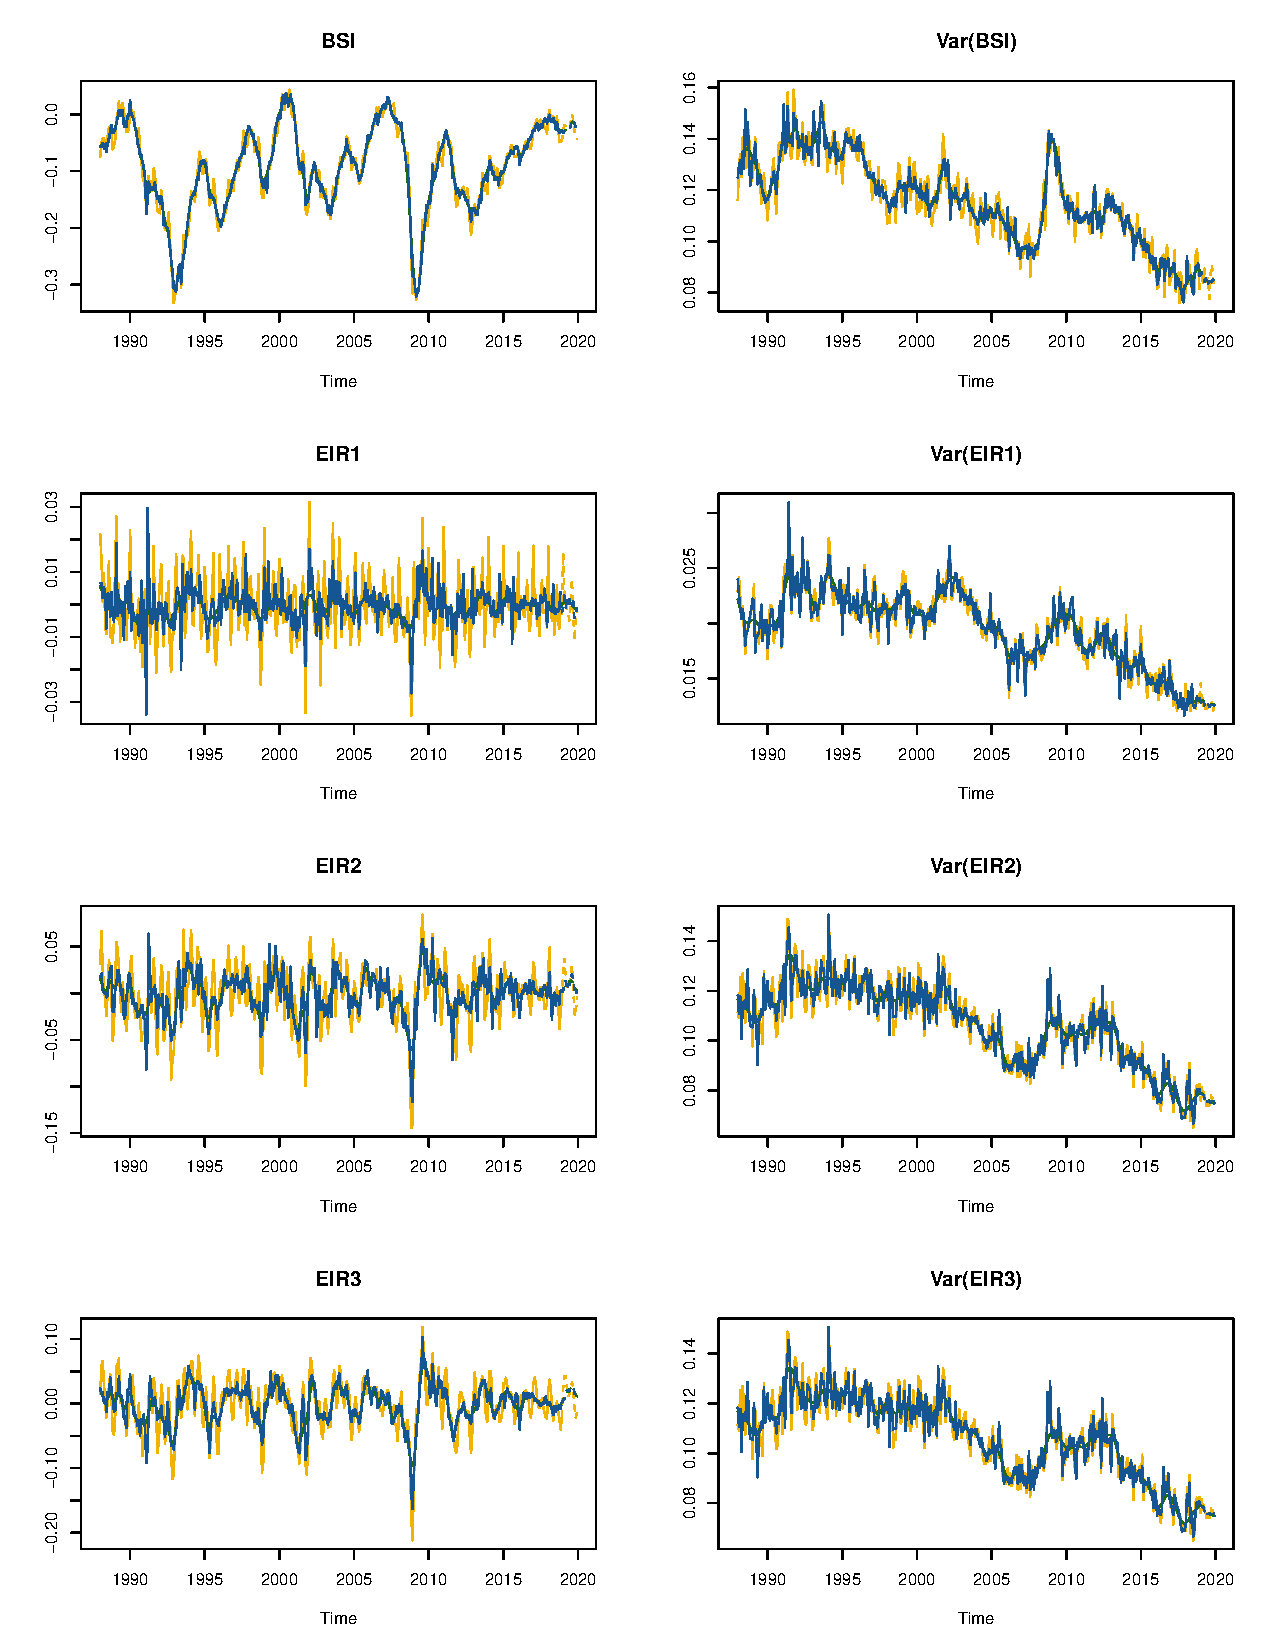
\includegraphics[scale=0.74]{Graphs/RJDemetra_plots.pdf}
    \caption{Plot of the industry business survey indicator (NS975), the indicator of the evolution of individual responses with the previous month (EIR1), two months (EIR2) and three months earlier (EIR3), with for each of them, their variance. The yellow lines are the raw variables, the blue lines the seasonally corrected variables and the green line are the trends of the variables.}
    \label{fig:seasonal ajusted rjdemetra}
\end{figure}


\section{Non-Response}

% Non-response is a large domain of research when it comes to surveys. The theory converges to agree that there are three different ways non-response can be present. Responses can be missing completely at random, missing at random, or missing not at random. Missing completely at random is usually hard to assume while missing not at random can be hard to account for.

% Considering the business survey, the non-response was explored, but since it's not the subject of the thesis, it will not be looked into more in dept.

The non-response of the business survey can be decomposed into two; non-participation to the survey and participants not responding to the survey.

Non-participation to the survey is difficult to study since not much trace is kept of the companies refusing to participate in the survey. As explained in the first chapter, the selection of participants uses stratification to account for the population at study. 
There is a bias that can come from the selection procedure since the survey is voluntary based, which means that if companies more prompt and motivated to participate are companies with a different profile compared to not motivated companies, there could be an issue.
The potential bias would be limited since the business survey is a panel survey and is interpreted as such.

Non-response of participants is another issue. 
Since the participants, in this case, dont answer a certain month but continue the survey, it can also be called non-monotone missingness.
The solution applied by the NBB in case of non-response, is to assume that the respondent would have answered the same as the previous month, the method is called "Last Observation Carried Forward" (LOCF). 
The theory regarding missing observations states three different ways non-response can be present. Responses can be missing completely at random (MCAR), missing at random (MAR), or missing not at random (MNAR). Missing completely at random is usually hard to assume while missing not at random can be hard to account for.
In the case of the business survey, the LOCF technique assumes that observations are missing completely at random. This method is not the most efficient and unbiased but has the advantage of been very simple and have more data (compared to considering the missing observations as NA's). 

There is a large effort made by the NBB to contact respondents and send them reminders to make sure that non-response is as small as possible.
The response rate is usually around 95\%, which is quite high for a survey, therefore it can be assumed that non-response is not very important in the business survey.

% Before concluding it, since the mean study is the evolution rather than the indicator in itself, we plotted the non-response with the evolution of the year on year GDP to see if there seems to be a relation between the two. For example, we could expect more or less non-response during crises or in certain economic situations. Since the main interest of the BSI is to explain business cycles,




\section{Dropout and Attrition}

Dropout and Attrition are related to the structure and organisation of the survey. 
As explain in \autoref{sec:Recruitment of participants}, one's participants are recruited to participate in the business survey, they stay as long as they want. This brings two potential issues: companies who leave the survey create a bias (dropout) and companies change of answering behaviour over time (attrition).

\subsection{Dropout}

The National Bank doesn't keep track from reasons why participants leave the survey. From discussions with the responsible persons for the survey at the NBB, the two mean reasons companies are leaving the survey are; (1) the company going bankrupt, acquired or merged and (2) the responsible person at the company leaves his job and the new contact person doesn't see the interest in participating in the survey.
This is an issue since it means that it's a certain type of company that leaves the survey. If this type of profile has a different opinion or respond differently than the remaining companies this will create bias. 


It could be argued that the bias is very diffused, due to the small number of companies leaving the survey each month. Again the fact that it's the evolution of the BSI that is important, means that the bias would be very small for each month (but if a longer period is taken into account, then the bias would become larger). 

% we are only comparing month to month evolution, and when the business survey is published, the 3-4 last year are showed.

Since it isn't the subject of this work, it will not be further look into this bias, but it will be recommend to have a closer look into this for future research.

\subsection{Attrition}


\nocite{warren_panel_2012}

Attrition, also called Panel Conditioning, is present when participants change there behaviour between different rounds of surveys. 
A very interesting master thesis was done about the Belgian labour force survey, where attrition was found to be significant \citep{priyana_hardjawidjaksana_investigating_2019}.
The Belgian labour force survey was convenient to test for attrition since the survey is answered by participants exactly four times with a lag of six months.
It was shown that indeed attrition was present in the survey.

In the case of the industry business survey, it's harder to test for it since their were only two major periods of recruitment for the period at interest (1988 - 2018); in the early 1990 and around 2000 with some companies been recruited outside those periods. Other sectors have the same issue.


\begin{table}[htp!]  \centering \footnotesize 
  \caption{Correlation of time with different indicators} 
  \label{tab:correlation attrition} 
\begin{tabular}{@{\extracolsep{5pt}} cccccc} 
\\[-1.8ex]\hline 
\hline \\[-1.8ex] 
 & GDP\_year & BSI & Var(BSI) & EIR & Var(EIR) \\ \hline \\[-1.8ex] 
Time & $-0.339$ & $0.133$ & $-0.807$ & $0.039$ & $-0.705$ \\ 
\hline \\[-1.8ex] 
\end{tabular} 
\end{table} 

An interesting approach to explore attrition and dropout is by looking at the correlations of the variances over time.
In \autoref{tab:correlation attrition} it can be seen that there is a very large negative correlation between time and the variance of the BSI and the variance of the EIR. This can be interpreted as companies agreeing more and more over time and changing less and less there answers.
Without making any conclusions, the variance of BSI and the variance of EIR seems to show the presence of dropout bias and/or attrition.

Same can be observed in Var(BSI) and Var(EIR) plots in \autoref{fig:seasonal ajusted rjdemetra} where, aside of the peak of variance during the economic crises of 2008, there is a general tendency of decreasing of the variance of the BSI and the different variances of EIR after the beginning of the century, the last time there was a large recruitment done.

The variance shows here an interest, it can be used to better understand the survey and the behaviour of respondents.
When looking at only the evolution of the business survey indicator, it's not possible to measure the vivacity of the survey.

It would be interesting to dive more into these issues, but this will be left for further research. 
In the context of this paper, it's important to notice the potential importance of attrition and dropout in the industry business survey and the importance of the variances to account for it.



\chapter{Exploratory Analysis}

The previous chapter already did some of the exploratory analysis.
Further observations of the different variables at hand will be done is a short descriptive statistics section.
In the second part, correlations among the variables will be looked at, and the last part will focus on autocorrelation.


\section{Descriptive Statistics}

\begin{table}[!htbp]  \centering \footnotesize 
  \caption{Descriptive Statistics} 
  \label{tab:descriptive statistics} 
\begin{tabular}{@{\extracolsep{5pt}}lccccccc} 
\\[-1.8ex]\hline 
\hline \\[-1.8ex] 
Statistic & \multicolumn{1}{c}{N} & \multicolumn{1}{c}{Mean} & \multicolumn{1}{c}{St. Dev.} & \multicolumn{1}{c}{Min} & \multicolumn{1}{c}{Pctl(25)} & \multicolumn{1}{c}{Pctl(75)} & \multicolumn{1}{c}{Max} \\ 
\hline \\[-1.8ex] 
YoY GDP     & 124       & 1.936 & 1.634 & $-$3.809 & 1.218 & 3.000 & 5.119 \\ 
BSI         & 372       & $-$0.094 & 0.075 & $-$0.321 & $-$0.141 & $-$0.033 & 0.037 \\ 
Var(BSI)    & 372       & 0.116 & 0.017 & 0.076 & 0.107 & 0.129 & 0.154 \\ 
EIR1        & 372       & $-$0.0003 & 0.006 & $-$0.034 & $-$0.004 & 0.003 & 0.030 \\ 
Var(EIR1)   & 372       & 0.020 & 0.003 & 0.012 & 0.017 & 0.022 & 0.031 \\ 
EIR2        & 372       & $-$0.001  & 0.024 & $-$0.116 & $-$0.013 & 0.013 & 0.064 \\ 
Var(EIR2)   & 372       & 0.107 & 0.016 & 0.067 & 0.095 & 0.119 & 0.151 \\ 
EIR3        & 372  & $-$0.002  & 0.031 & $-$0.163 & $-$0.018 & 0.018 & 0.103 \\ 
Var(EIR3)   & 372       & 0.123 & 0.019 & 0.075 & 0.109 & 0.137 & 0.166 \\ 
\hline \\[-1.8ex] 
\end{tabular} 
\end{table} 

The variables at hand are obtained from the industry business survey and take into account the four questions available on \autopageref{Appendix: Question NS975 description}, as explained in \autoref{sec:Questionnaire}.
The different variables are unweighted, seasonally corrected (see \autoref{sec:seasonal correction}) and is obtained for 30 years, from 1988 to 2018.
The year on year GDP calculation was explained from GDP byt the calculation in \autoref{eq:YoY GDP} and is here obtained for the Belgian economy.

The different variables at hand are summarised in \autoref{tab:descriptive statistics}. The YoY GDP has only one third as many observations as the other variables since it's a quarterly measure, while the survey is monthly. 
The table shows the scale of the different variables, for example, the industry BSI, over 30 years, never went higher than 0.037 and never lower than -0.321.

The different variables are plotted in \autoref{plot:variables}, where it can be seen that the business survey indicator follows quite well the evolution of YoY GDP. 
The other variables, seem to react to major changes in GDP but are more volatile.

\begin{figure}[!htbp]
    \centering
    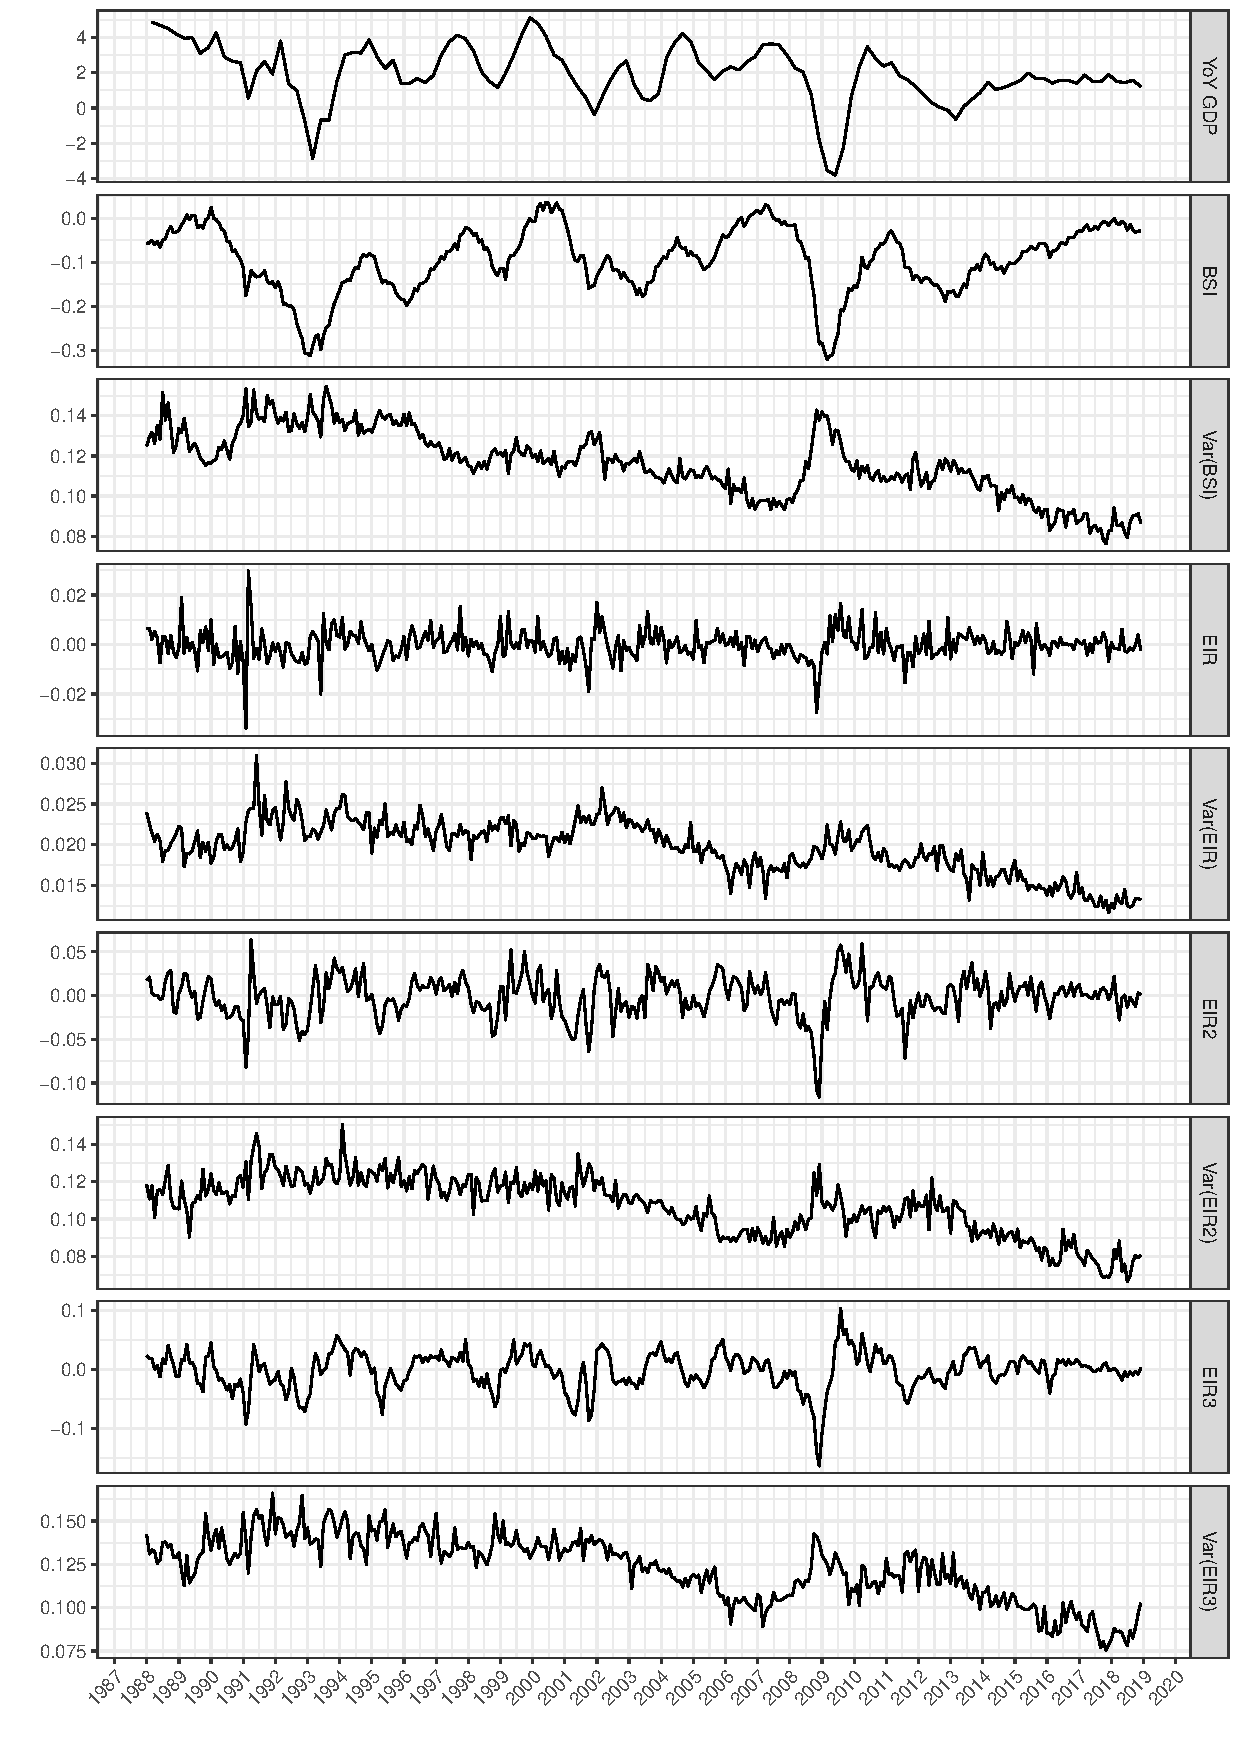
\includegraphics[scale=0.75]{Graphs/variables.pdf}
    \caption{Plot of the time series of YoY GDP, the BSI, the variance of the BSI and different EIR's (taking 1, 2 or 3 months differences) and their variance
    for the period 1988 to 2018}
    \label{plot:variables}
\end{figure}



\section{Correlation Analysis}

Belgian industry claims 25\% of the labour force in Belgium and was shown as a good indicator of the year to year GDP
\cite{de_greef_national_2009}.

\begin{figure}[H]
    \centering
    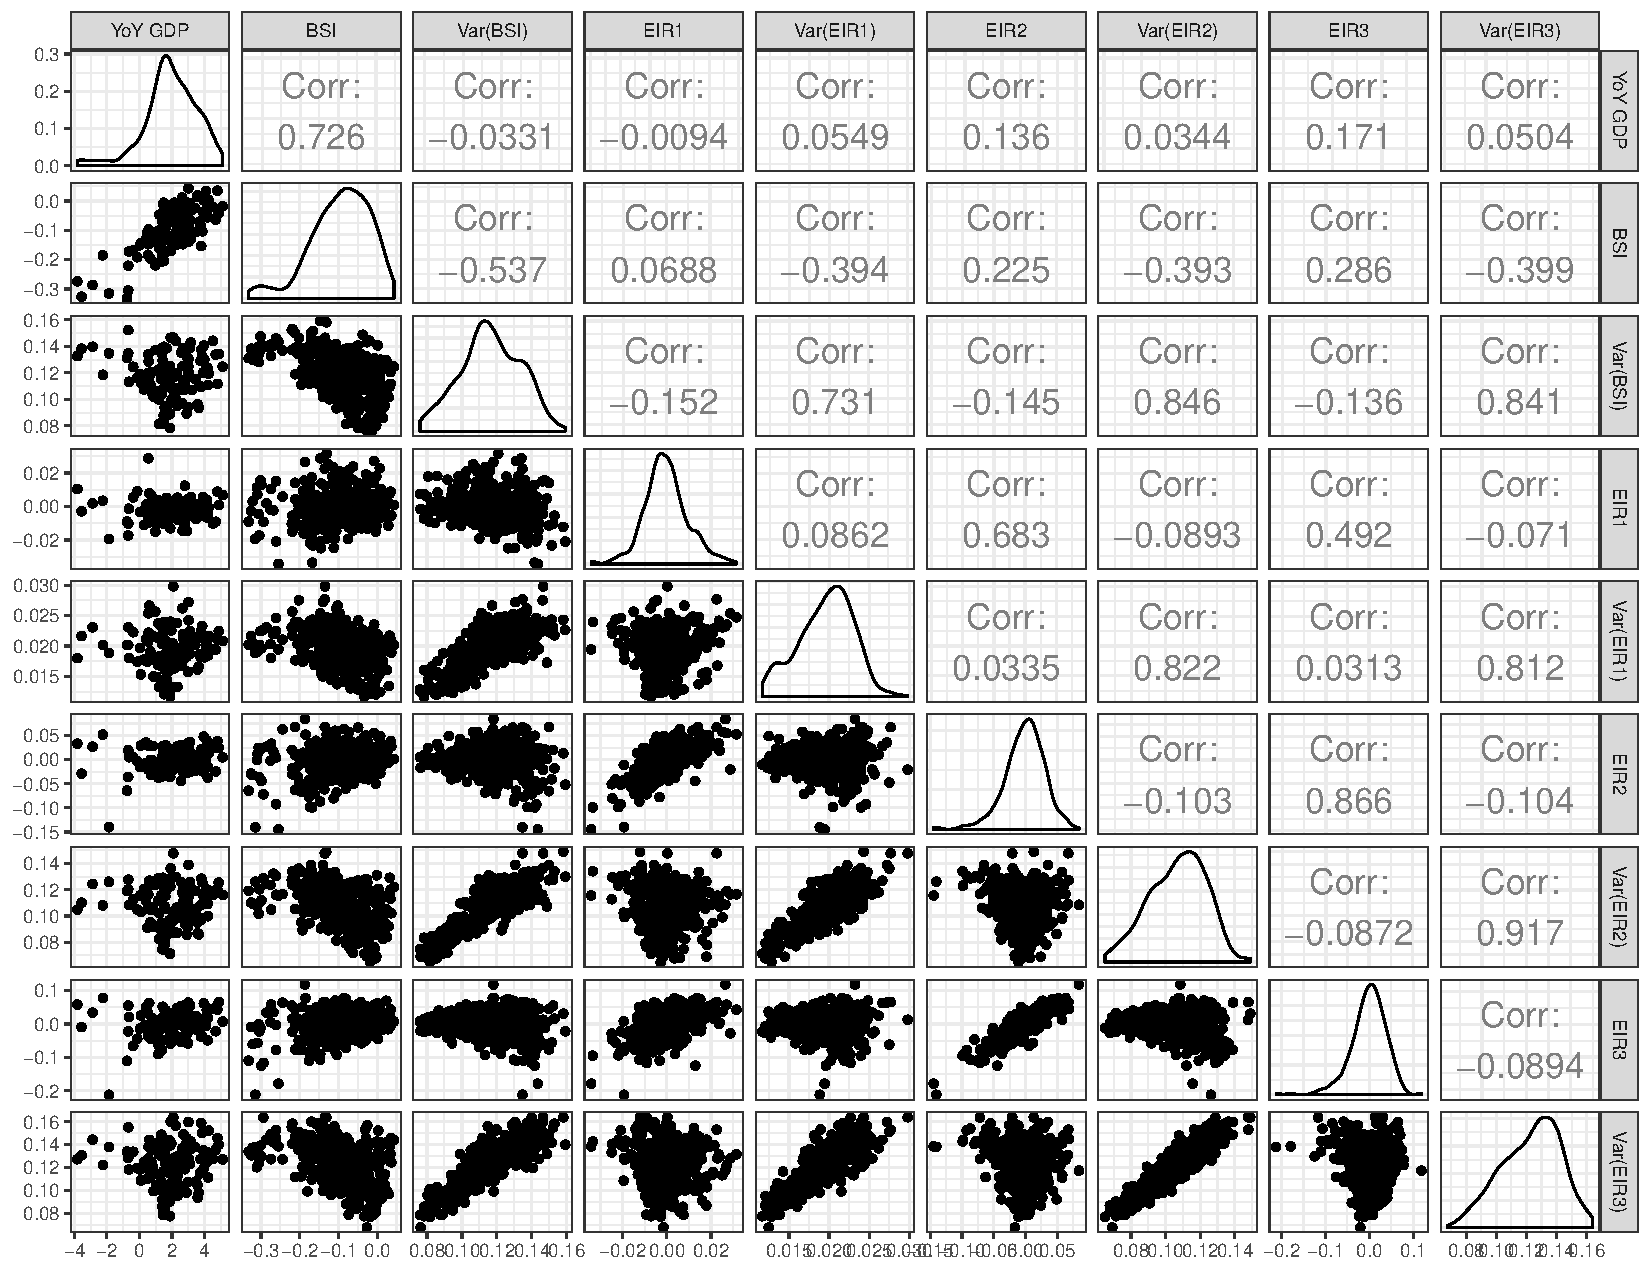
\includegraphics[scale=0.5]{Graphs/corr_indicators.pdf}
    \caption{Correlation plot of the YoY GDP, the business survey indicator and its variance, and the evolution of individual responses for 1,2 and three months lag and its according variances}
    \label{fig:corr indicators}
\end{figure}

\autoref{fig:corr indicators} shows the correlation matrix and plots of the different variables at hand. 
Several observations can be done.
First, it can be seen that the correlation between the business survey indicator and YoY GDP is very high while other variables have a rather small correlation with YoY GDP.

The correlation between the BSI and its variance is also high, this can be explained to some extent by the different observations done in \autoref{sec:properties variance}.
The same can not be said about the correlation between the EIR and its variance since their correlation is small for the three different measures of EIR.

As could be foreseen, the correlations between EIR1, EIR2 and EIR3 and the correlations between Var(EIR1), Var(EIR2) and Var(EIR3) are high. There calculation and data used been quite close.

The correlation between the different types of variances is also high, which can mean that they contain quite similar information.
With this definition, it's interesting to look at the correlation between the BSI and the EIR since it's almost equal to zero. This can be interpreted as the two variables containing different information.

\section{Autocorrelation}

Autocorrelation, also known as serial correlation, is the correlation between an observation at time $t$ and previous observations.

The method used here is to estimate the autocorrelation function and plot it, the result can be seen in \autoref{fig:ACF}, where the correlation of a variable with its previous lags is shown. 
In the case of the YoY GDP, one lag (X axis of the plot) is three months since the variable is quarterly, while for the other variables the lag corresponds to one month.
Several variables have high autocorrelation. The variances are highly correlated over time, as is the BSI. 
On the other hand, YoY GDP is slightly correlated with its three previous quarter values. 
For EIR1, the observations are not correlated at all with their previous observations. It can be observed that the autocorrelation increases by the number of months taking into account for the EIR.

...


\begin{figure}[!htbp]
    \centering
    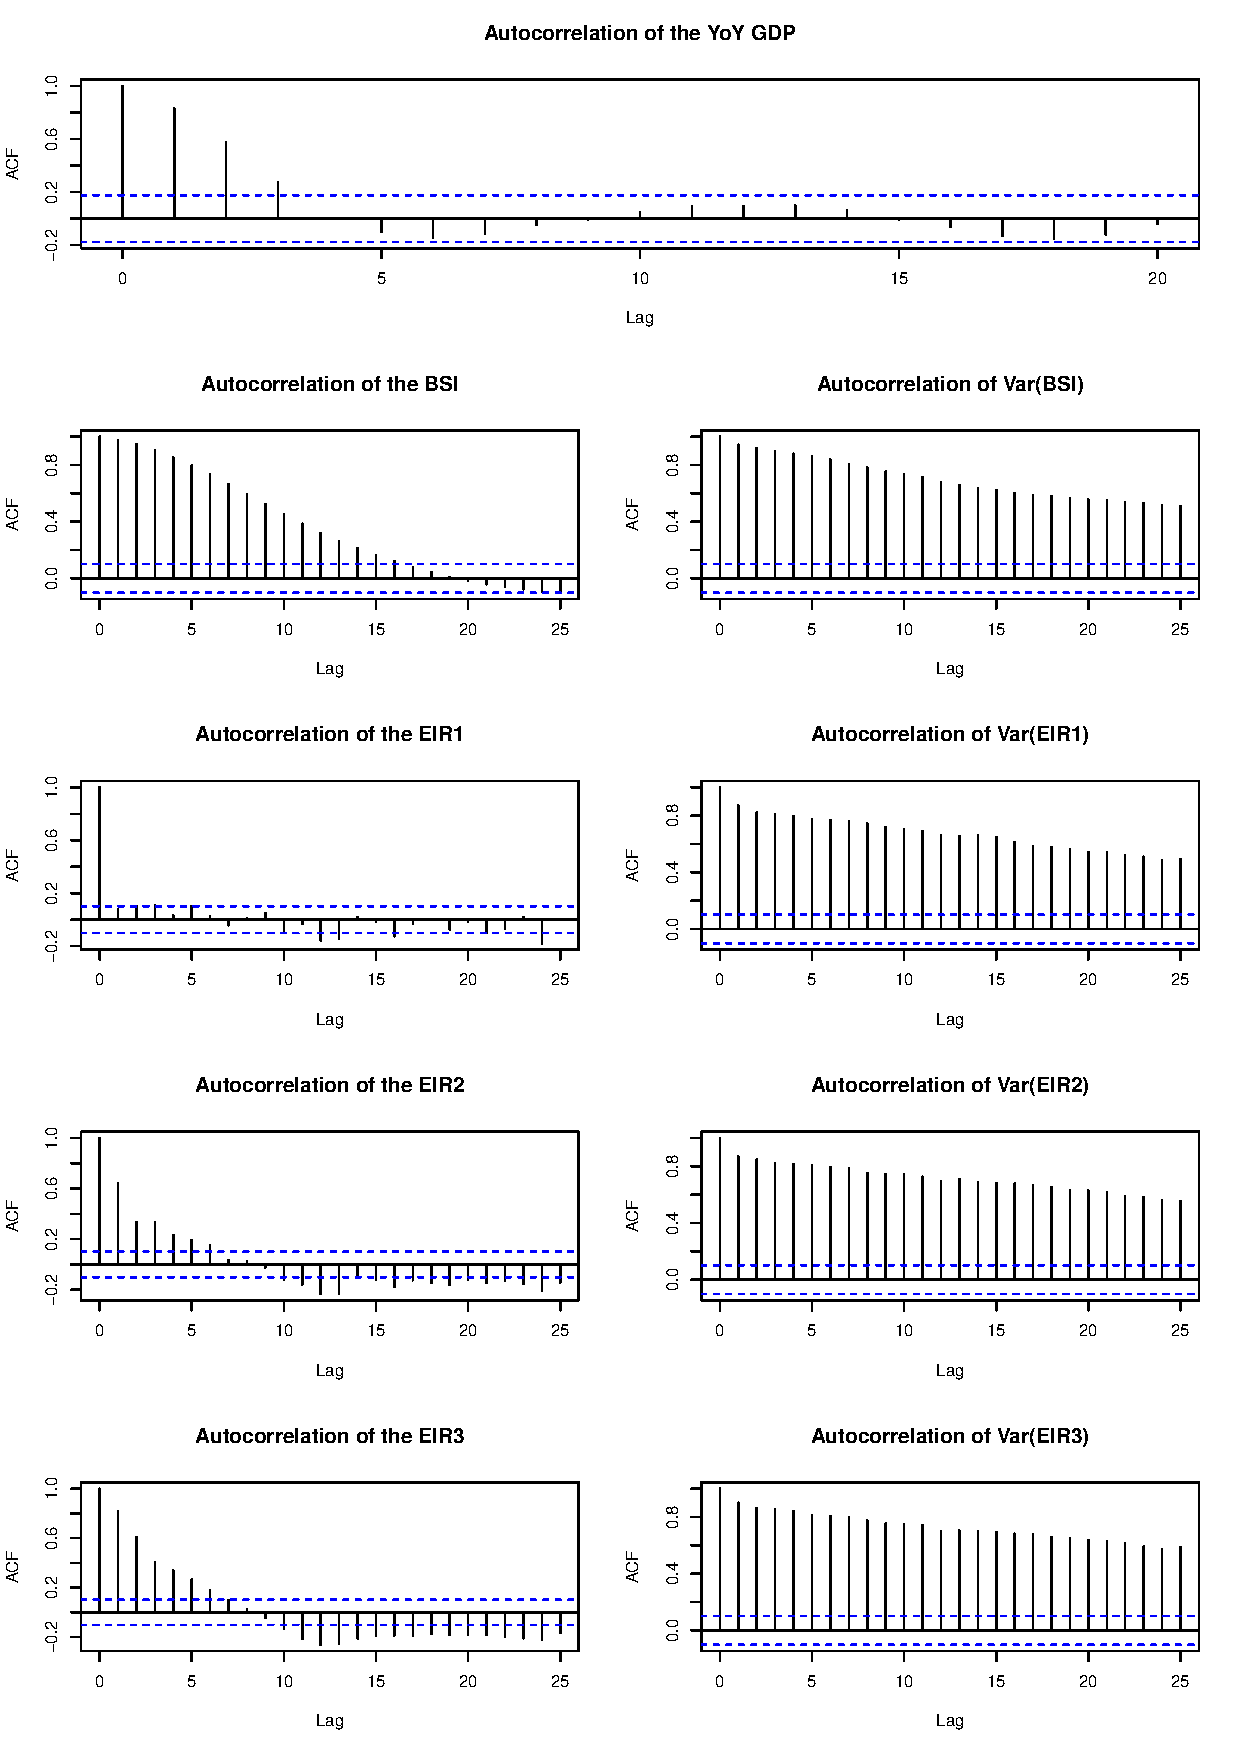
\includegraphics[scale=0.75]{Graphs/ACF.pdf}
    \caption{Autocorrelation plots for YoY GDP, the BSI, Var(BSI), EIR1, Var(EIR1), EIR2, Var(EIR2), EIR3 and Var(EIR3)}
    \label{fig:ACF}
\end{figure}



\chapter{Linear Models}

This chapter uses a linear models to test the pertinence of the different variables at hand in the short term prediction of the evolution of GDP.

As mention in \autoref{sec:nowcasting}, where nowcasting was discussed, there exists a large variety of different predictive models used in econometrics to predict the National Growth based on some explanatory variables.
The National Bank of Belgium for example, developed a State-Space model available in JDemetra+ \citep{de_antonio_liedo_nowcasting_2014}. Other well-known methods are ARIMA models, MIDAS and much more.

The interest of the research at hand, is to explore the utility of the variance of the business survey indicator, the evolution of individual responses and its variance.

To achieve this objective, it's better to use a model that account easily for the interest of each variable. The idea here is not to find the best model but rather to see if including the new indicators in a certain model will improve predictions.
Therefore, the linear model is preferred.

This chapter will begin with proposing five different models, one simple model where only the BSI is used as regressor, and then four potential models that include other regressors.
Several test statistics will be looked at and used to compare the different models and understand if the new regressors added to the model, improve the model fit and the estimations.
A method of model selection will then by applied to see if it decides to include the new regressors into the model aside from from the BSI.
The last part will use out-of-sample estimation to check if the results from the previous tests are robust.

\section{Method}

The quarterly year on year GDP is set in the last month of the quarter. This is the common way to go to take a reasonable approach and still have some predictive properties.
Indeed, when looking at \autoref{fig:time of the data}, it can be seen that with the linear model it's possible to estimate quarterly YoY GDP one month before it's published. 
This means that the model will be estimated only with the indicators of the last month of each quarter. One the model is estimated, it's then possible to make predictions or estimations of YoY GDP for each month.




\begin{figure}[!htp]
     \centering \footnotesize
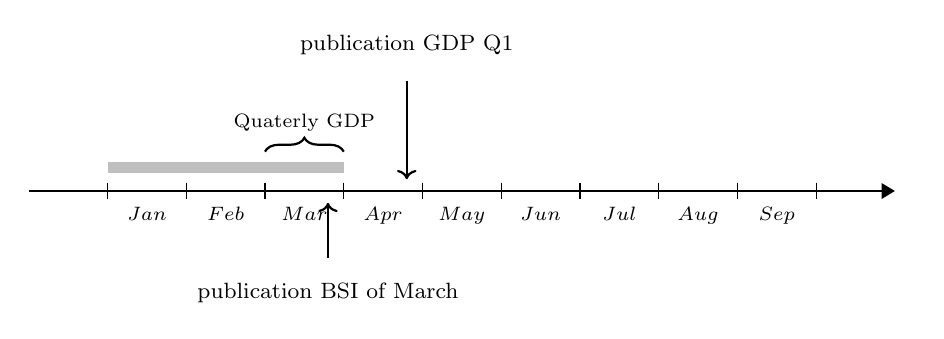
\begin{tikzpicture}  \footnotesize
% draw horizontal line   
\draw[thick, -Triangle] (0,0) -- (\ImageWidth,0) node[font=\scriptsize,below left=3pt and -8pt]{ };
% draw vertical lines
\foreach \x in {1,...,10}
\draw (\x cm,3pt) -- (\x cm,-3pt);
\foreach \x/\descr in {1.5/Jan, 2.5/Feb, 3.5/Mar, 4.5/Apr, 5.5/May, 6.5/Jun, 7.5/Jul, 8.5/Aug,9.5/Sep}
\node[font=\scriptsize, text height=1.75ex,
text depth=.5ex] at (\x,-.3) {$\descr$};
% colored bar up
\foreach \x/\perccol in
{1/100,2/75,3/25}
\draw[lightgray, line width=4pt] 
(\x,.3) -- +(1,0);

% braces
\draw [thick ,decorate,decoration={brace,amplitude=5pt}] (3,0.5)  -- +(1,0) 
       node [black,midway,above=4pt, font=\scriptsize] {Quaterly GDP};
% time of publication
\node[align=center] at (4.8,1.85) {publication GDP Q1};
\draw [thick,->] (4.8,1.4) -- (4.8,0.15);
\node[align=center] at (3.8,-1.3) {publication BSI of March};
\draw [thick,->] (3.8,-0.85) -- (3.8,-0.15);
\end{tikzpicture}
    \caption{Timeline of the observations of GDP and the business survey and their publication}
    \label{fig:time of the data}
\end{figure}


\section{Linear Models}

The linear regression can be written as follow

\begin{eqnarray}
    \text{YoY GDP}_{t} = \beta_0 + \sum^n_{i = 1}
       \beta_{i} X_{t} + \epsilon_t 
\end{eqnarray}

Where $\beta_{0}$ is a constant, $\beta_{i}$  are the different regression coefficients of the monthly predictors ($X_{t}$) and $\epsilon_t$ is the error term.

This model is quite a good example of basic nowcasting, since it's modelling data that's happening at the same time, but since there is a lag of a month in the publication of GDP, it can be used to predict a month in advance, the published GDP.

It can also be used to estimate GDP monthly. Ones a linear model is obtained, based only on quarterly data, it can then be applied to all the available data, and a prediction can be done for each month.
In real life, this means that at the end of January, when the results of GDP are published for the last semester of the previous year, the linear model can predict YoY growth for the month of January. Therefore it's not forecasting, since it doesn't predict the future, but predict what will be published

The first approach here is to propose five different models and compare them.
The simplest model takes as unique regressor, the business survey indicator

\begin{equation} \tag{Model 1}
    \text{YoY GDP}_{t} = \beta_0 + \beta_{1} \BSI_{t} + \epsilon_t \label{eq:model1}
\end{equation}

This will be the reference model. A model where only the BSI is used to predict GDP growth (YoY GDP). It will be compared to the following models.

A model that takes the business survey indicator and its variance as regressors

\begin{equation} \tag{Model 2}
    \text{YoY GDP}_{t} = \beta_0 + \beta_{1} \BSI_{t}  + \beta_{2} \Var(\BSI)_{t} + \epsilon_t \label{eq:model2}
\end{equation}

And three different models where the three evolution of individual responses with their variances are each time added to the previous model

\begin{equation} \tag{Model 3}
    \text{YoY GDP}_{t} = \beta_0 + \beta_{1} \BSI_{t}  + \beta_{2} \Var(\BSI)_{t} + \beta_{3} \EIR1_{t}  + \beta_{4} \Var(\EIR1)_{t} + \epsilon_t \label{eq:model3}
\end{equation}

\begin{equation} \tag{Model 4}
    \text{YoY GDP}_{t} = \beta_0 + \beta_{1} \BSI_{t}  + \beta_{2} \Var(\BSI)_{t} + \beta_{5} \EIR2_{t}  + \beta_{6} \Var(\EIR2)_{t} + \epsilon_t \label{eq:model4}
\end{equation}

\begin{equation} \tag{Model 5}
    \text{YoY GDP}_{t} = \beta_0 + \beta_{1} \BSI_{t}  + \beta_{2} \Var(\BSI)_{t} + \beta_{7} \EIR3_{t}  + \beta_{8} \Var(\EIR3)_{t} + \epsilon_t  \label{eq:model5}
\end{equation}

\begin{table}[htbp!] \centering \footnotesize
  \caption{Linear Regression Results for the period 1988 to 2018} 
  \label{tab:models comparaison 1} 
\begin{tabular}{@{\extracolsep{2pt}}lD{.}{.}{-3} D{.}{.}{-3} D{.}{.}{-3} D{.}{.}{-3} D{.}{.}{-3} } 
\\[-1.8ex]\hline 
\hline \\[-1.8ex] 
 & \multicolumn{5}{c}{Linear Regression} \\ 
\cline{2-6} 
\\[-1.8ex] & \multicolumn{5}{c}{year on year GDP} \\ 
\\[-1.8ex] & \multicolumn{1}{c}{(\ref{eq:model1})} & \multicolumn{1}{c}{(\ref{eq:model2})} & \multicolumn{1}{c}{(\ref{eq:model3})} & \multicolumn{1}{c}{(\ref{eq:model4})} & \multicolumn{1}{c}{(\ref{eq:model5})}\\ 
\hline \\[-1.8ex] 
 Constant & 3.429^{***} & -1.740^{***} & -1.821^{***} & -1.756^{***} & -1.729^{***} \\ 
  & (0.160) & (0.631) & (0.615) & (0.635) & (0.633) \\ 
  & & & & & \\ 
 BSI & 15.773^{***} & 21.443^{***} & 21.548^{***} & 21.310^{***} & 21.044^{***} \\ 
  & (1.317) & (1.252) & (1.224) & (1.306) & (1.313) \\ 
  & & & & & \\ 
 Var(BSI) &  & 49.102^{***} & 36.477^{***} & 40.631^{***} & 38.777^{***} \\ 
  &  & (5.869) & (8.089) & (11.895) & (11.081) \\ 
  & & & & & \\ 
 EIR1 &  &  & -28.718^{**} &  &  \\ 
  &  &  & (13.792) &  &  \\ 
  & & & & & \\ 
 Var(EIR1) &  &  & 78.555^{**} &  &  \\ 
  &  &  & (35.187) &  &  \\ 
  & & & & & \\ 
 EIR2 &  &  &  & -0.709 &  \\ 
  &  &  &  & (3.878) &  \\ 
  & & & & & \\ 
 Var(EIR2) &  &  &  & 9.213 &  \\ 
  &  &  &  & (11.207) &  \\ 
  & & & & & \\ 
 EIR3 &  &  &  &  & 1.290 \\ 
  &  &  &  &  & (2.610) \\ 
  & & & & & \\ 
 Var(EIR3) &  &  &  &  & 9.401 \\ 
  &  &  &  &  & (8.598) \\ 
  & & & & & \\ 
\hline \\[-1.8ex] 
Observations & \multicolumn{1}{c}{124} & \multicolumn{1}{c}{124} & \multicolumn{1}{c}{124} & \multicolumn{1}{c}{124} & \multicolumn{1}{c}{124} \\ 
R$^{2}$ & \multicolumn{1}{c}{0.540} & \multicolumn{1}{c}{0.709} & \multicolumn{1}{c}{0.728} & \multicolumn{1}{c}{0.711} & \multicolumn{1}{c}{0.712} \\ 
Adjusted R$^{2}$ & \multicolumn{1}{c}{0.537} & \multicolumn{1}{c}{0.704} & \multicolumn{1}{c}{0.719} & \multicolumn{1}{c}{0.701} & \multicolumn{1}{c}{0.702} \\ 
Resid. Std. Er. & \multicolumn{1}{c}{1.112} & \multicolumn{1}{c}{0.889} & \multicolumn{1}{c}{0.866} & \multicolumn{1}{c}{0.894} & \multicolumn{1}{c}{0.891} \\ 
AIC & \multicolumn{1}{c}{382.292} & \multicolumn{1}{c}{327.699} & \multicolumn{1}{c}{323.086} & \multicolumn{1}{c}{330.907} & \multicolumn{1}{c}{330.293} \\ 
BIC & \multicolumn{1}{c}{390.753} & \multicolumn{1}{c}{338.980} & \multicolumn{1}{c}{340.008} & \multicolumn{1}{c}{347.829} & \multicolumn{1}{c}{347.215} \\ 
\hline 
\hline \\[-1.8ex] 
\textit{Note:}  & \multicolumn{5}{r}{$^{*}$p$<$0.1; $^{**}$p$<$0.05; $^{***}$p$<$0.01} \\ 
\end{tabular} 
\end{table} 

The estimates can be seen in \autoref{tab:models comparaison 1} for the five regressions. Some goodness of fit measures are also available. 
Those first results show the limited interest of EIR2 and EIR3 since the model with EIR1 and its variance (\autoref{eq:model3}) is better performing according to all the results than the two other models (\autoref{eq:model4} and \autoref{eq:model5}).

The other observation that can be done is that the interest of the variance in the prediction seems significant since adding, next to the information of the business survey, increases the Adjusted R$^2$ by 0.151. The model is also better according to AIC and BIC results.






\begin{table}[!htbp]
    \centering \footnotesize
    \caption{Accuracy Measures}
    \label{tab:accuracy measures}
\begin{tabular}{@{\extracolsep{5pt}} cccccccc} 
\\[-1.8ex]\hline 
\hline \\[-1.8ex] 
                 & RMSE & MAE & MPE & MAPE & MASE \\ \hline
\ref{eq:model1} & 1.103 &0.93 &-27.657 & 86.696 & 0.764 \\
\ref{eq:model2} & 0.878 &0.697 & -10.923 & 61.185 & 0.573 \\
\ref{eq:model3} & 0.848 &0.674 & -12.455 & 55.698 & 0.554 \\
\ref{eq:model4} & 0.875 &0.699 & -12.757 & 62.707 & 0.574 \\
\ref{eq:model5} & 0.873 &0.689 & -9.83 & 59.311 & 0.566 \\ \hline
    \end{tabular}
\end{table}

\autoref{tab:accuracy measures} shows some more measures of goodness-of- fit; the Root Mean Squared Error (RMSE), the Mean Absolute Error (MAE), the Mean Percentage Error (MPE), Mean Absolute Percentage Error (MAPE) and Mean Absolute Scaled Error (MASE).
All give similar result as before, \ref{eq:model3} is performing best according to all the measures except in MPE.

The results for \ref{eq:model2} are quite close to the results of \ref{eq:model3}. There is no clear best model between the two.

In \autoref{fig:predictions1} the prediction of YoY GDP according to the three first models are shown for the whole period. It can be seen that model 2 and 3 are better performing that model 1, while model 2 and 3 deliver quite similar predictions.

\begin{figure}[!htbp]
    \centering
    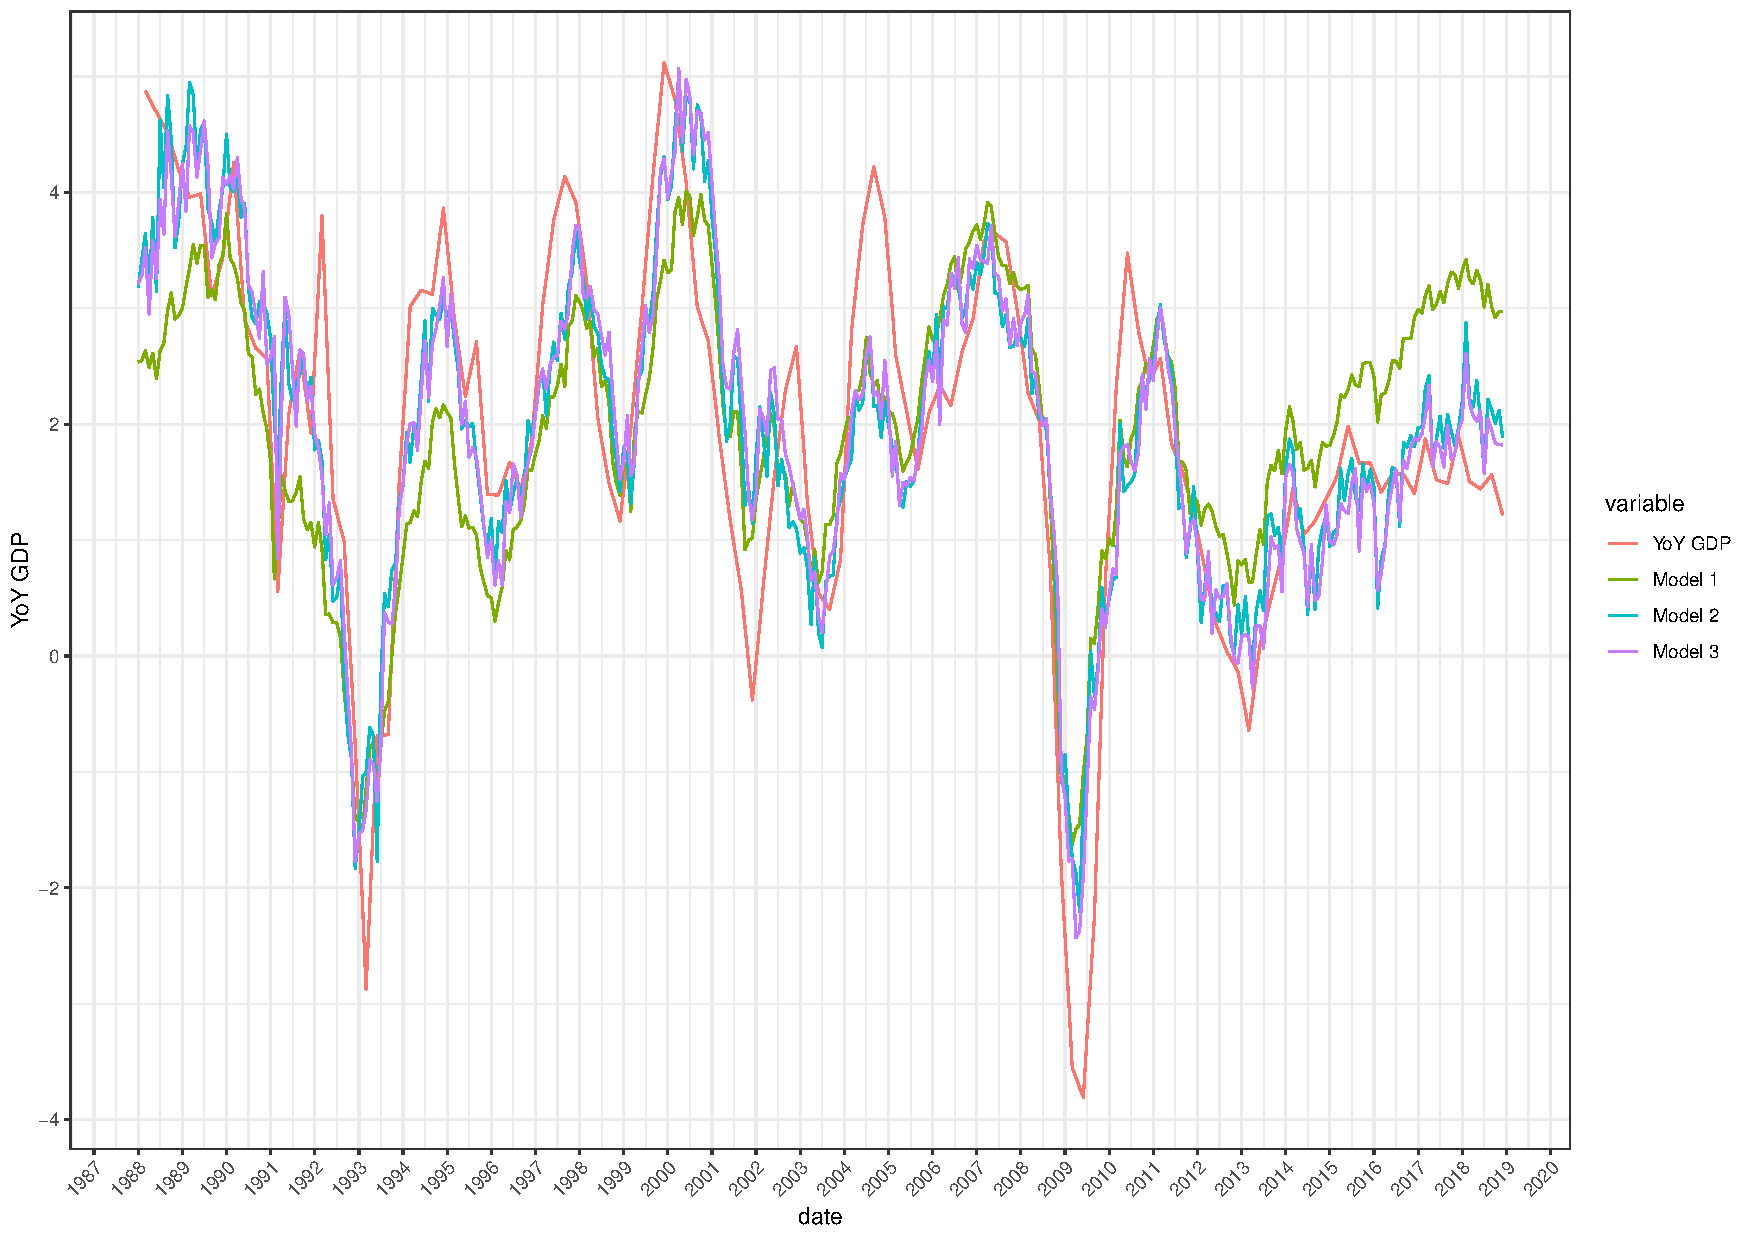
\includegraphics[scale=0.5]{Graphs/predictions1.pdf}
    \caption{Plot of year on year GDP and the different estimation from model 1, 2 and 3}
    \label{fig:predictions1}
\end{figure}

\subsubsection{Diebold-Mariano Test}

The Diebold-Mariano statistical test \citep{diebold_comparing_1995} is well known to compare forecast accuracy of different models. 
it determine whether forecasts of a certain model are significantly better than another model by using the residuals.

The parameters of the test are forecast horizon = 1, loss function power = 2 and alternative hypothesis: two.sided and the results can be seen in \autoref{tab:Diebold Mariano 1}


\begin{table}[htp!]
    \caption{Diebold-Mariano tests for the models referred to in \ \autoref{tab:models comparaison 1} }
    \label{tab:Diebold Mariano 1}
     \centering \footnotesize
    \begin{tabular}{| r | c c c c c |}
    \cline{2-6}
 \multicolumn{0}{r|}{p-values}	& \ref{eq:model1} & \ref{eq:model2} & \ref{eq:model3} & \ref{eq:model4} & \ref{eq:model5} \\ \cline{1-6}
 \ref{eq:model1} & 1 & 5.126e-06  & 2.586e-06 & 6.352e-06 & 5.602e-06\\ 
 \ref{eq:model2} &   & 1  & 0.2055 & 0.6836 & 0.5147 \\
 \ref{eq:model3} &   &   & 1 & &   \\
 \ref{eq:model4} &   &   &  0.1613 & 1 & 0.7876 \\
 \ref{eq:model5} &   &   & 0.3017 &   & 1 \\ \cline{1-6}
\end{tabular}
\end{table}






\subsubsection{Model Selection}

! graph representation !

Since there are a large among of different possible models when having eight different regressors, some procedure needs to be chosen to look for the best model.

The method applied here is a step procedure where AIC is used to select the best model.
Three different selection algorithms will be applied; (1) forward, (2) backward and  (3) both of the step() procedure in R. 
The three methods are all based on Akaike's information criterion (AIC) as a measure of goodness of fit. They differ in the sense that the first (1) starts from a model with no regressors and adds one by one the regressors that improve the most the model fit, the second (2) does the opposite, it starts with the full model and takes out the variables that don't improve the model fit and the last (3) is a mixed of the two previous methods.

The results of the three different methods converge to the model already proposed refered to as \ref{eq:model3}, where BSI, Var(BSI), EIR1 and Var(EIR1) are the regressors that.

From the different results, it can already be stated that EIR1 and its variance are bringing more in the modelling of the YoY GDP than EIR2 and EIR3 with their variances.

It was also seen that the variance of the BSI improves the model quite largely and that EIR1 and its variance can also add some information.

Following those results, there are two good candidates; \autoref{eq:model2} and \ref{eq:model3}. Those are the two models that will be further looked into and compared to the simplest model only including the BSI (\autoref{eq:model1}).



\subsubsection{Out-of-Sample Performances}

To know if the results from the linear model are robust, two out-of-sample estimation will be performed.

The first will use the period 1988 to 2000 to estimate the model, and its predictions for that period and for 1988 to 2018 will be compared using Diebold-Mariano test.
The period was chose since it's only 12 years long, and will have to be accurate for the next 18 years. The situation it's representing, is if, since January, each model was used to make prediction, which would deliver the best results.

See if attrition and dropout, who could be assumed as been more present after 2000, since that was the last recruitment period (see graphs appendix)

The same will then be done for the period 1988 until 2012. The year 2012 was chosen after having a closer look at \autoref{fig:predictions1}, where it seems that most of the improvement brought by the models including more than only the BSI, is from 2012 on. Therefore it's interesting to see how the different models perform without taking that period into account.

% Without making any conclusions, a possible interpretation of this improvement brought by the variance of the BSI in the estimation for the period after 2012, could be explained by attrition or dropout.

\begin{table}[htp!]
     \caption{Diebold-Mariano tests for the models estimated with the data from 1988 to 2000, applied to the data from 1988-2000 and 1988-2018 with the estimates from \autoref{tab:model comparaison 2000}}
    \label{tab:Diebold Mariano 2}
    \centering \footnotesize
    \begin{tabular}{| r | c c c | c c c |}
 \multicolumn{1}{r}{} &    \multicolumn{3}{c}{\textbf{1988-2000}} &    \multicolumn{3}{c}{\textbf{1988-2018}} \\ \cline{2-7}
 \multicolumn{0}{r|}{p-values}	& \ref{eq:model1} & \ref{eq:model2} & \ref{eq:model1} & \ref{eq:model1} & \ref{eq:model2} & \ref{eq:model3} \\ \cline{1-7}
 \ref{eq:model1} & 1 & 0.2203 & 0.08282  & 1 & 1.867e-11 & 5.555e-11 \\ 
 \ref{eq:model2} &   & 1  	& 0.2886  	&   & 1 & 0.000745 \\
 \ref{eq:model3} &   &    & 1 &   &   & 1   \\ \cline{1-7}
\end{tabular}
\end{table}

\autoref{tab:Diebold Mariano 2} shows that the models, estimated with the data from 1988 to 2000, there predictions aren't significantly different from each others, while if the model is applied to the whole period of 1988 to 2018, \ref{eq:model3} is significantly better than \ref{eq:model1} and \ref{eq:model2}.

The estimates and fitted plot can be seen on \autopageref{tab:model comparaison 2000}.
If exclusively the period 1988-2000 is taken into account, \ref{eq:model2} and \ref{eq:model3} are only slightly better than \ref{eq:model1} according to most of the statistics.
It can then be seen, from the plot, and even more from the Diebold-Mariano tests, that \ref{eq:model2} and \ref{eq:model3} outperform \ref{eq:model3} after that period, even if the data used for the estimation of the model only uses the data available before 2000.




On the other hand, \autoref{tab:Diebold Mariano 3} shows the Diebold-Mariano test p-values for the model estimated with the data until 2012. The results for the period 1988-2012 and 1988-2018 are quite similar and come to the same conclusion, \ref{eq:model2} and \ref{eq:model3} outperform \ref{eq:model1}. While \ref{eq:model3} is not significantly better than \ref{eq:model2}.

The estimates and fitted plot can be seen on \autopageref{tab:model comparaison 2012}. 



\begin{table}[htp!]
    \caption{Diebold-Mariano tests for the models estimated with the data from 1988 to 2012, applied to the data from 1988-2012 and 1988-2018 with the estimates from \autoref{tab:model comparaison 2012}}
    \label{tab:Diebold Mariano 3}
     \centering \footnotesize
    \begin{tabular}{| r | c c c | c c c |}
 \multicolumn{1}{r}{} &    \multicolumn{3}{c}{\textbf{1988-2012}} &    \multicolumn{3}{c}{\textbf{1988-2018}} \\ \cline{2-7}
 \multicolumn{0}{r|}{p-values}	& \ref{eq:model1} & \ref{eq:model2} & \ref{eq:model1} & \ref{eq:model1} & \ref{eq:model2} & \ref{eq:model3} \\ \cline{1-7}
 \ref{eq:model1} & 1 & 0.00956 & 0.007979 & 1 & 1.269e-07 & 1.751e-07 \\ 
 \ref{eq:model2} &   & 1  & 0.2813 &   	  & 1 & 0.09632 \\
 \ref{eq:model3} &   &    & 1 &   &   & 1   \\ \cline{1-7}
\end{tabular}
\end{table}















\chapter{Conclusion}

After presenting the business survey and the business survey barometer, it was seen that
the variance of the business survey indicator showed some interesting interpretation and properties. 
Because the business survey has only three possible answers per questions, the variance is related to the mean and bounded between 0 and 1.

The evolution of individual responses was developed and explained.
It's variance was shown as also having a mean-variance relation and been bounded between 0 and 2.

After correction the different variables and indicators for seasonal effects, the two different variances where shown to be potential indicators of dropout and/or attrition.

The correlation analysis confirmed the relation between the indicator and its variance since there correlation is quite large. It was also seen that none of the new indicators had a high correlation with YoY GDP while the industry BSI has a correlation slightly higher than 0.7 with the measure of growth.

The variance of the BSI, the EIR and its variance are more volatile than the business survey indicator when looking at there evolution over time.

Considering the predictive power of the different variables, it was seen that as expected the business survey indicator is a good predictor, and that its variance would have increase the prediction accuracy.

% Those results have to be taken carefully due to the potential harm of dropout bias and/or attrition.

It was seen that if in 2000, it was decided to use linear models to do nowcasting of the YoY GDP, and that model would be used until this day, the model including the BSI, its variance, the EIR and its variance would have outperformed a model only using the BSI.





\chapter{Discussion}



The Belgian industry business survey indicator was shown as very good indicator of the YoY GDP, confirming previous research.

% The present research showed that adding the variance has some potential interest in better understanding the survey, more precisely the respondents behaviour. This behaviour seems to show that dropout and attrition can have a effect on 

\subsubsection{Recruitment procedure and panel data}

The recruitment of respondents to the survey was explained and reasons where given for not using a random sampling method. Nevertheless this decision has several implications that could be further studied.

The selection of new participants by waves of recruitment is an issue if it's assumed that there is attrition and dropout bias.
A constant recruitment of new participants, would attenuated the potential bias. 
Literature has shown that respondents behaviour changes related to the participation period and some simple descriptive statistics from the business survey seemed to confirm the presence the previous assumption. For those reasons,further research regarding this issue would be of a great benefit to better understand and correct for those issues.

\subsubsection{Develop indicator by taking to different question into account that are linked}

% \subsubsection{EIR that takes more periods into account}

Regarding the indicator of the evolution of individual responses (EIR), further research and development could take two forms. 

One would be to develop an indicator that will be able to take more than two months into account. This was explored but a consistent and interpretable indicator could not be found. 

Another method would be to use different questions. In the business survey some questions are linked between each other; questions concern the level of production in the past, some the present level of production and other questions relate to there predictions for the following months. 
A new indicator could be a measure of the accuracy of the predictions of the respondents and could be used to compare the different participants or different periods.


% \subsubsection{Take question 1 (Q18) out}

% Some descriptive statistics and research not included in this paper showed the small correlation of question 18 of the industry indicator with YoY GDP.

\subsubsection{LOCF or other non-response methods}
Considering non-response, some other technique than "Last Observation Carried Forwards" could be used. 
Multiple Imputations would be an interesting approach to handle non-response in the business survey as was done for the German business survey in \cite{seiler_microdata_2013}. It could decrease the bias and increase accuracy. 
This could be interesting topic to explore.


\subsubsection{Variance predictive power or correction dropout, attrition}

The linear regression showed the significant importance of the variance. the out-of-sample tests showed that the importance of variance is mostly for the period after 2012. Which coincide with the period where no new recruitment's where done for this indicator. During that period there was more probably attrition and dropout bias, which the variance of the indicator is a kind of measure of. The question that can not be answered here but should further be looked at is whether the variance has a predictive power of if it acts as a correction for the attrition and/or dropout bias.

The linear regression also showed that the indicator of the evolution of individual responses and its variance slightly improve the model. 
The interpretation that can be done is very interesting, those two indicators would be recommended to better understand how respondents respond in a survey.

% Adapting a methodology proposed in Das et al. (2011), this paper uses panel refreshments as a natural experiment to determine whether trends in stated utility measures observed in panel data are genuine or rather caused by measurement issues. \cite{van_landeghem_test_2014}

\subsubsection{Techniques to correct for dropout and attrition bias out}




\subsubsection{Other modelling}

The next step considering predictive power of the new indicators is including them in other predictive models and see how they perform

Markov Switching, State-Space Models, MIDAS, Bridge Models ....

Markov Switching 
\citep{hamilton_new_1989} applied to the French business survey \cite{bardaji_constructing_2009}

Combine mixed models and Markov Chain for Panel Data \citep{de_haan-rietdijk_use_2017} 


A comparison of mixed frequency approaches for nowcasting Euro area macroeconomic aggregates
\cite{foroni_comparison_2014} 


Nonparametric Tests of Panel Conditioning and Attrition Bias in Panel Surveys
\cite{das_nonparametric_2011}



Bayesian estimation \citep{bialowolski_bayesian_nodate}


\nocite{binder_business_1995}
\nocite{dresse_survey_2008}
\nocite{lemasson_enquete_2017}
\nocite{mevik_uncertainty_2004}

\bibliographystyle{apa}
\bibliography{references}
 


  
\begin{appendix}
  \listoffigures
  \listoftables
\end{appendix}


\chapter*{Appendix}

\section*{Questions taken into account for the calculation of the industry business survey}
\label{Appendix: Question NS975 description}

originally numbered question 18, 27, 32 and 33 (see \autopageref{Questionnaire2018}), for simplicity numbered here as 1, 2, 3 and 4.
Note that the first question is interpreted in the opposite way from the three other. Having a higher stock than normal is considered a "negative" answer while lower stock is considered "positive".


\subsubsection*{Course and assessment}
\begin{enumerate}
    \item Your current stock of this product will you consider, for the season, as: \\
    $\Square$ higher than normal (too high) $\Square$ normal (sufficient) $\Square$ lower than normal (too low)
    
    \item Your current aggregate order position for this product is what you consider to be: \\
    $\Square$ higher than normal $\Square$ normal $\Square$ lower than normal
\end{enumerate}

\subsubsection*{Prospects for the next three months} 
\begin{enumerate}
\setcounter{enumi}{2}
    \item The personnel (workers and technicians) employed for the manufacture of this product will, according to you: \\
    $\Square$ be expanded $\Square$ remain unchanged $\Square$ be reduced
                        
    \item The demand of your customers for this product will, in your opinion:  \\
    $\Square$ be more important $\Square$ be equally important $\Square$ be less important \\\    
    as usual at that time of the year.
\end{enumerate}





\newpage
\section*{Further explanations regarding the variance of the business survey indicator, the indicator of the evolution of individual responses and its variance}
\label{chap:appendix:explain Var BSI and EIR}


When taking a very simplified situation where there are only two respondents over a 2 months period and only taking one question into account. 
We can take five different situations that will help to further understand and interpret the business survey indicator, the evolution of individual responses and there respective variances.
The five different situation have all a BSI equal to zero at time t, while different Var(BSI), EIR and Var(EIR). 
By looking at \autoref{tab:explanation of Var and BSI} and \autoref{fig:explanation of Var and BSI} it can be seen that in situation one everyone is neutral which means that all the indicators are equal to one.
Situation two is slightly different since the two respondents hardly disagree and keep the same answer over at $t-1$ and at $t$.


\begin{table}[H]
    \caption{Five possible situations of a simplified business survey with only two respondents over a two months period}
    \label{tab:explanation of Var and BSI}
    \centering
\begin{tabular}{c|c c c c c c} \footnotesize
situation    & respondent 1 & respondent 2           &  BSI & Var(BSI) & EIR & Var(EIR) \\ \hline
 1 & neutral $\rightarrow$ neutral & neutral $\rightarrow$ neutral & 0 & 0 & 0 & 0   \\
 2 & positive $\rightarrow$ positive & negative $\rightarrow$ negative & 0 & 1 & 0 & 0 \\
 3 & positive $\rightarrow$ negative & negative $\rightarrow$ positive & 0 & 1 & 0 & 4 \\
 4 & positive $\rightarrow$ neutral & positive $\rightarrow$ neutral & 0 & 0 & -1 & 0  \\
 5 & positive $\rightarrow$ neutral & negative $\rightarrow$ neutral & 0 & 0 & 0 & 1  \\
\end{tabular}
\end{table}
%
\begin{figure}[H]
        \centering
     \begin{subfigure}[t]{0.3\textwidth}
        \centering
    \begin{tikzpicture} \footnotesize
           \draw [thin, black, ->] (0,0) -- (0,4);    % draw y-axis line
            \draw [thin, black, ->] (0,0) -- (4,0);      % draw x-axis line
            \draw [draw=black,ultra thick] (0.5,2) -- (3.5,2);% draw the graph
            \node [left] at (0,0.7) {$-$};                % label y-intercept
            \node [left] at (0,2) {$0$};                % label y-intercept
            \node [left] at (0,3.3) {$+$};                % label y-intercept
            \node [below] at (0.5,0) {$t-1$};               % label x-intercept
            \node [below] at (3.5,0) {$t$};               % label x-intercept
    \end{tikzpicture}
    \caption{Situation 1}
    \end{subfigure}
    ~
        \begin{subfigure}[t]{0.3\textwidth}
        \centering
        \begin{tikzpicture} \footnotesize
           \draw [thin, black, ->] (0,0) -- (0,4);    % draw y-axis line
            \draw [thin, black, ->] (0,0) -- (4,0);      % draw x-axis line
            \draw [draw=black, thick] (0.5,0.7) -- (3.5,0.7);% draw the graph
            \draw [draw=black, thick] (0.5,3.3) -- (3.5,3.3);% draw the graph  
            \node [left] at (0,0.7) {$-$};                % label y-intercept
            \node [left] at (0,2) {$0$};                % label y-intercept
            \node [left] at (0,3.3) {$+$};                % label y-intercept
            \node [below] at (0.5,0) {$t-1$};               % label x-intercept
            \node [below] at (3.5,0) {$t$};               % label x-intercept
    \end{tikzpicture}
    \caption{Situation 2}
    \end{subfigure}
    ~
    \begin{subfigure}[t]{0.3\textwidth}
        \centering
        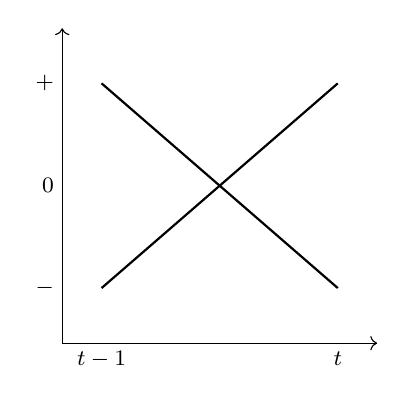
\begin{tikzpicture} \footnotesize
           \draw [thin, black, ->] (0,0) -- (0,4);    % draw y-axis line
            \draw [thin, black, ->] (0,0) -- (4,0);      % draw x-axis line
            \draw [draw=black, thick] (0.5,0.7) -- (3.5,3.3);% draw the graph
            \draw [draw=black, thick] (0.5,3.3) -- (3.5,0.7);% draw the graph  
            \node [left] at (0,0.7) {$-$};                % label y-intercept
            \node [left] at (0,2) {$0$};                % label y-intercept
            \node [left] at (0,3.3) {$+$};                % label y-intercept
            \node [below] at (0.5,0) {$t-1$};               % label x-intercept
            \node [below] at (3.5,0) {$t$};               % label x-intercept
    \end{tikzpicture}
    \caption{Situation 3}
    \end{subfigure}
    ~
    \begin{subfigure}[t]{0.3\textwidth}
        \centering
        \begin{tikzpicture} \footnotesize
           \draw [thin, black, ->] (0,0) -- (0,4);    % draw y-axis line
            \draw [thin, black, ->] (0,0) -- (4,0);      % draw x-axis line
            \draw [draw=black, ultra thick] (0.5,3.3) -- (3.5,2);% draw the graph  
            \node [left] at (0,0.7) {$-$};                % label y-intercept
            \node [left] at (0,2) {$0$};                % label y-intercept
            \node [left] at (0,3.3) {$+$};                % label y-intercept
            \node [below] at (0.5,0) {$t-1$};               % label x-intercept
            \node [below] at (3.5,0) {$t$};               % label x-intercept
    \end{tikzpicture}
    \caption{Situation 4}
    \end{subfigure}
  ~
        \begin{subfigure}[t]{0.3\textwidth}
        \centering
        \begin{tikzpicture} \footnotesize
           \draw [thin, black, ->] (0,0) -- (0,4);    % draw y-axis line
            \draw [thin, black, ->] (0,0) -- (4,0);      % draw x-axis line
            \draw [draw=black, thick] (0.5,3.3) -- (3.5,2);% draw the graph  
            \draw [draw=black, thick] (0.5,0.7) -- (3.5,2);% draw the graph  
            \node [left] at (0,0.7) {$-$};                % label y-intercept
            \node [left] at (0,2) {$0$};                % label y-intercept
            \node [left] at (0,3.3) {$+$};                % label y-intercept
            \node [below] at (0.5,0) {$t-1$};               % label x-intercept
            \node [below] at (3.5,0) {$t$};               % label x-intercept
    \end{tikzpicture}
    \caption{Situation 5}
    \end{subfigure}

      \caption{Plots of five possible situations of a simplified business survey with only two respondents over a two months period}
    \label{fig:explanation of Var and BSI}
\end{figure}


Situation three is again a situation where respondents disagree but now also change radically there answer over a two months period. So the two variances are at there highest.
Situation four is a situation where the two respondents where positive the previous month and are now both neutral. There variances are equal to zero since they both agree and they changed there answer the same but EIR is equal to -1 since compare to previous month they decreased there answer.
In situation five they disagreed largely the previous month but now are both neutral so only their variance of EIR is not equal to zero.

This explanation shows the interest of the four different indicators that each shown a different information about the responses.


\section*{?Attrition and dropout bias?}

To go slightly further in studying attrition and dropout several graphs are presented here and interpreted. 
This part was included in appendix due to it relative large amount of subjective interpretation and it lack of theory to back its development.

\autoref{fig:participants var bsi} shows the evolution of the number of participants and the variance of the BSI. As was seen in \autoref{tab:correlation attrition} the variance decreases with time. When looking at the graph its



\autoref{fig:participants var eir} is quite similar to \autoref{fig:participants var bsi} with this time the var(EIR) plotted rather than var(BSI).


!!
add BSI to the plot
!!


\begin{figure}[htp!]
    \centering
    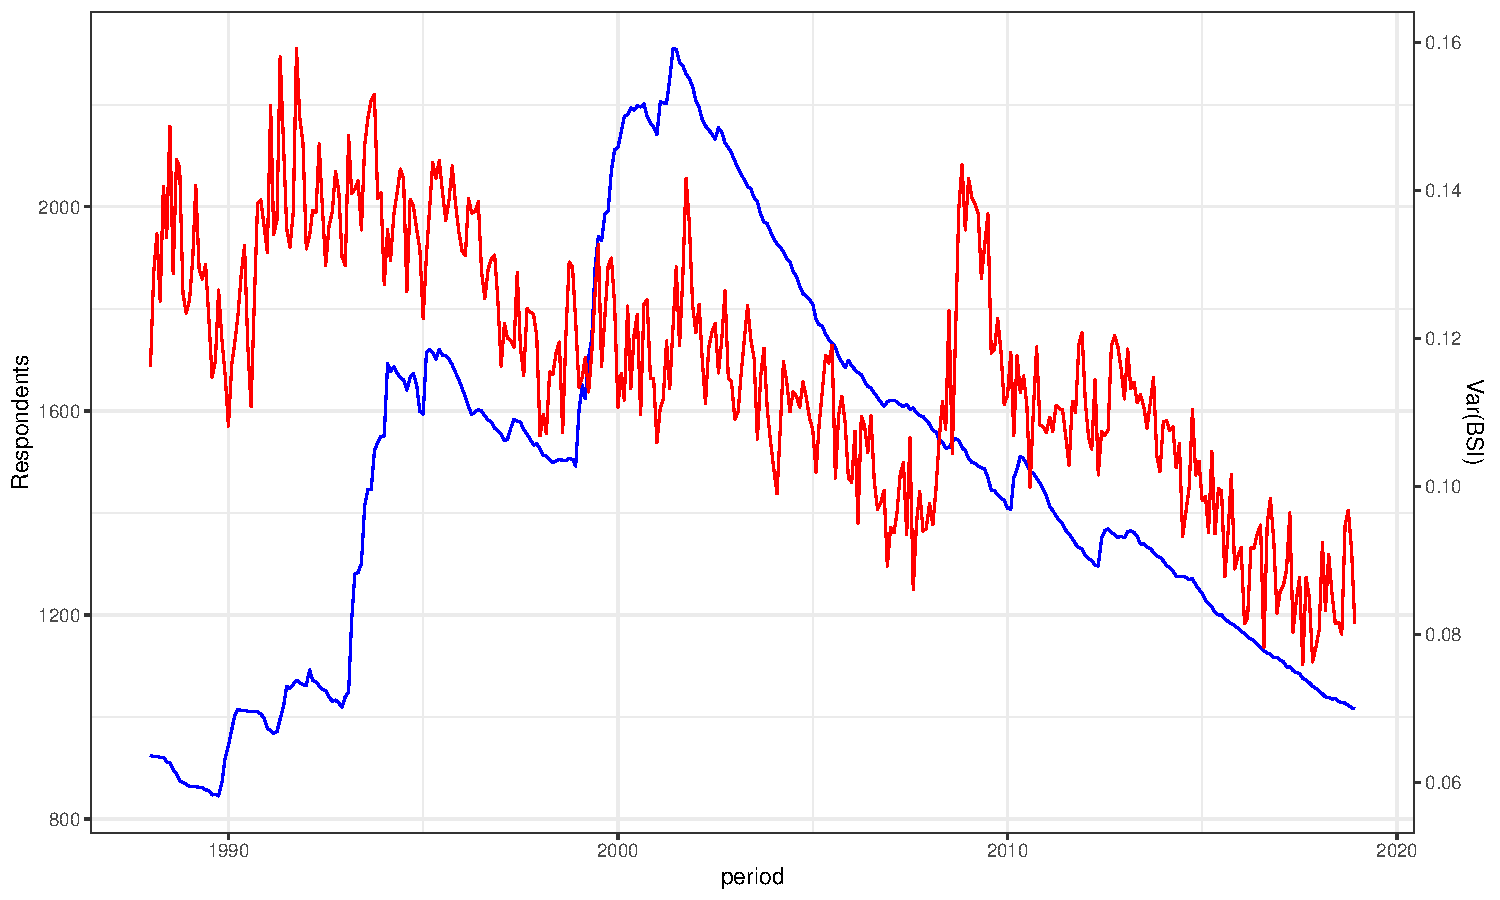
\includegraphics[scale=0.5]{Graphs/participants_var_bsi.pdf}
    \caption{participants var bsi}
    \label{fig:participants var bsi}
\end{figure}

\begin{figure}[H]
    \centering
    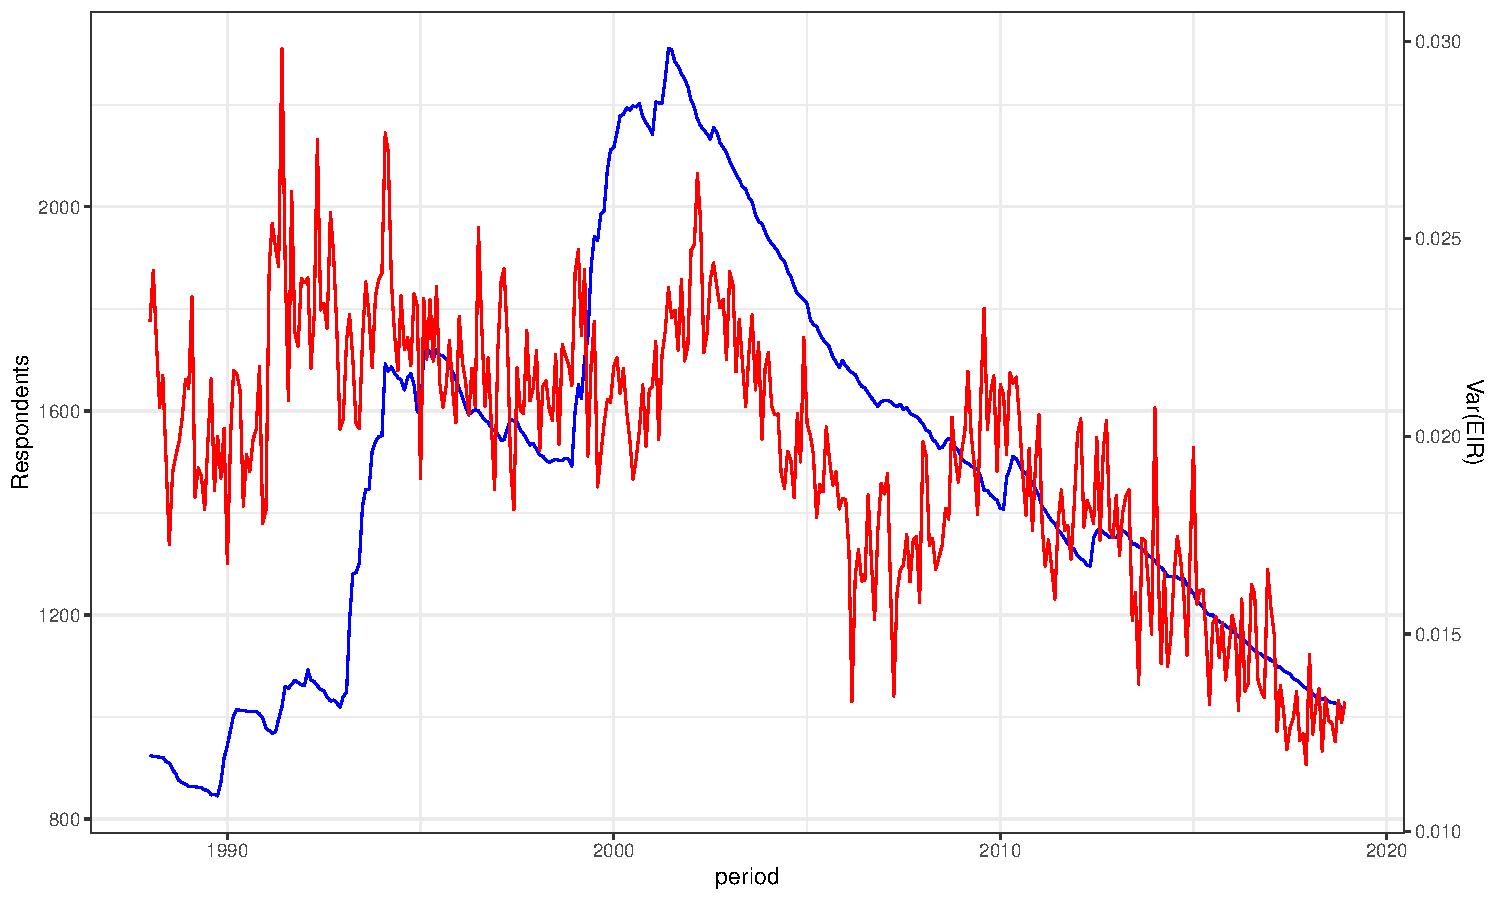
\includegraphics[scale=0.5]{Graphs/participants_var_eir.pdf}
    \caption{participants var eir}
    \label{fig:participants var eir}
\end{figure}




\newpage
\begin{figure}[H]
    \centering
    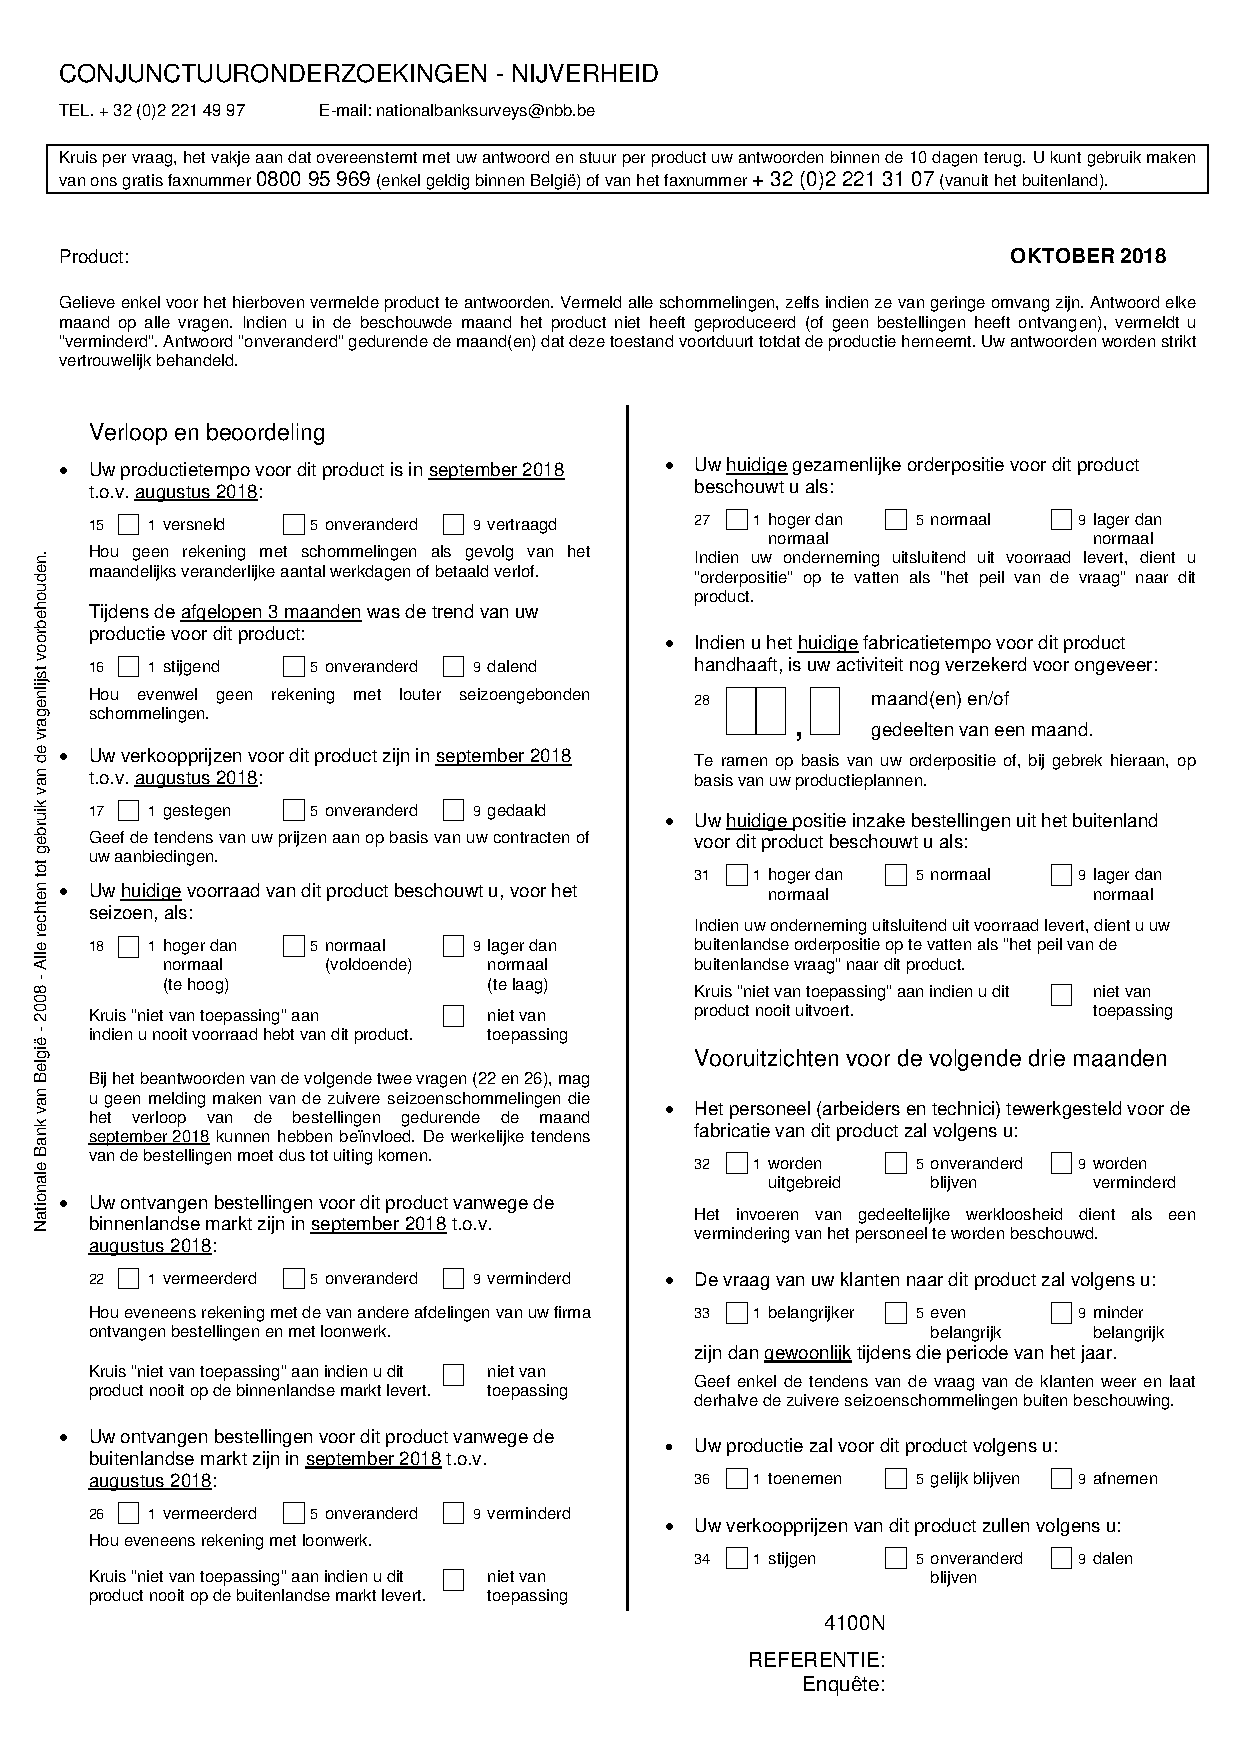
\includegraphics[scale=0.75]{Images/IndustryN.pdf}
    \caption{The Business Survey Questionnaire in Dutch for the Industrial Sector in 2018}
    \label{Questionnaire2018}
\end{figure}

\begin{figure}[H]
    \centering
    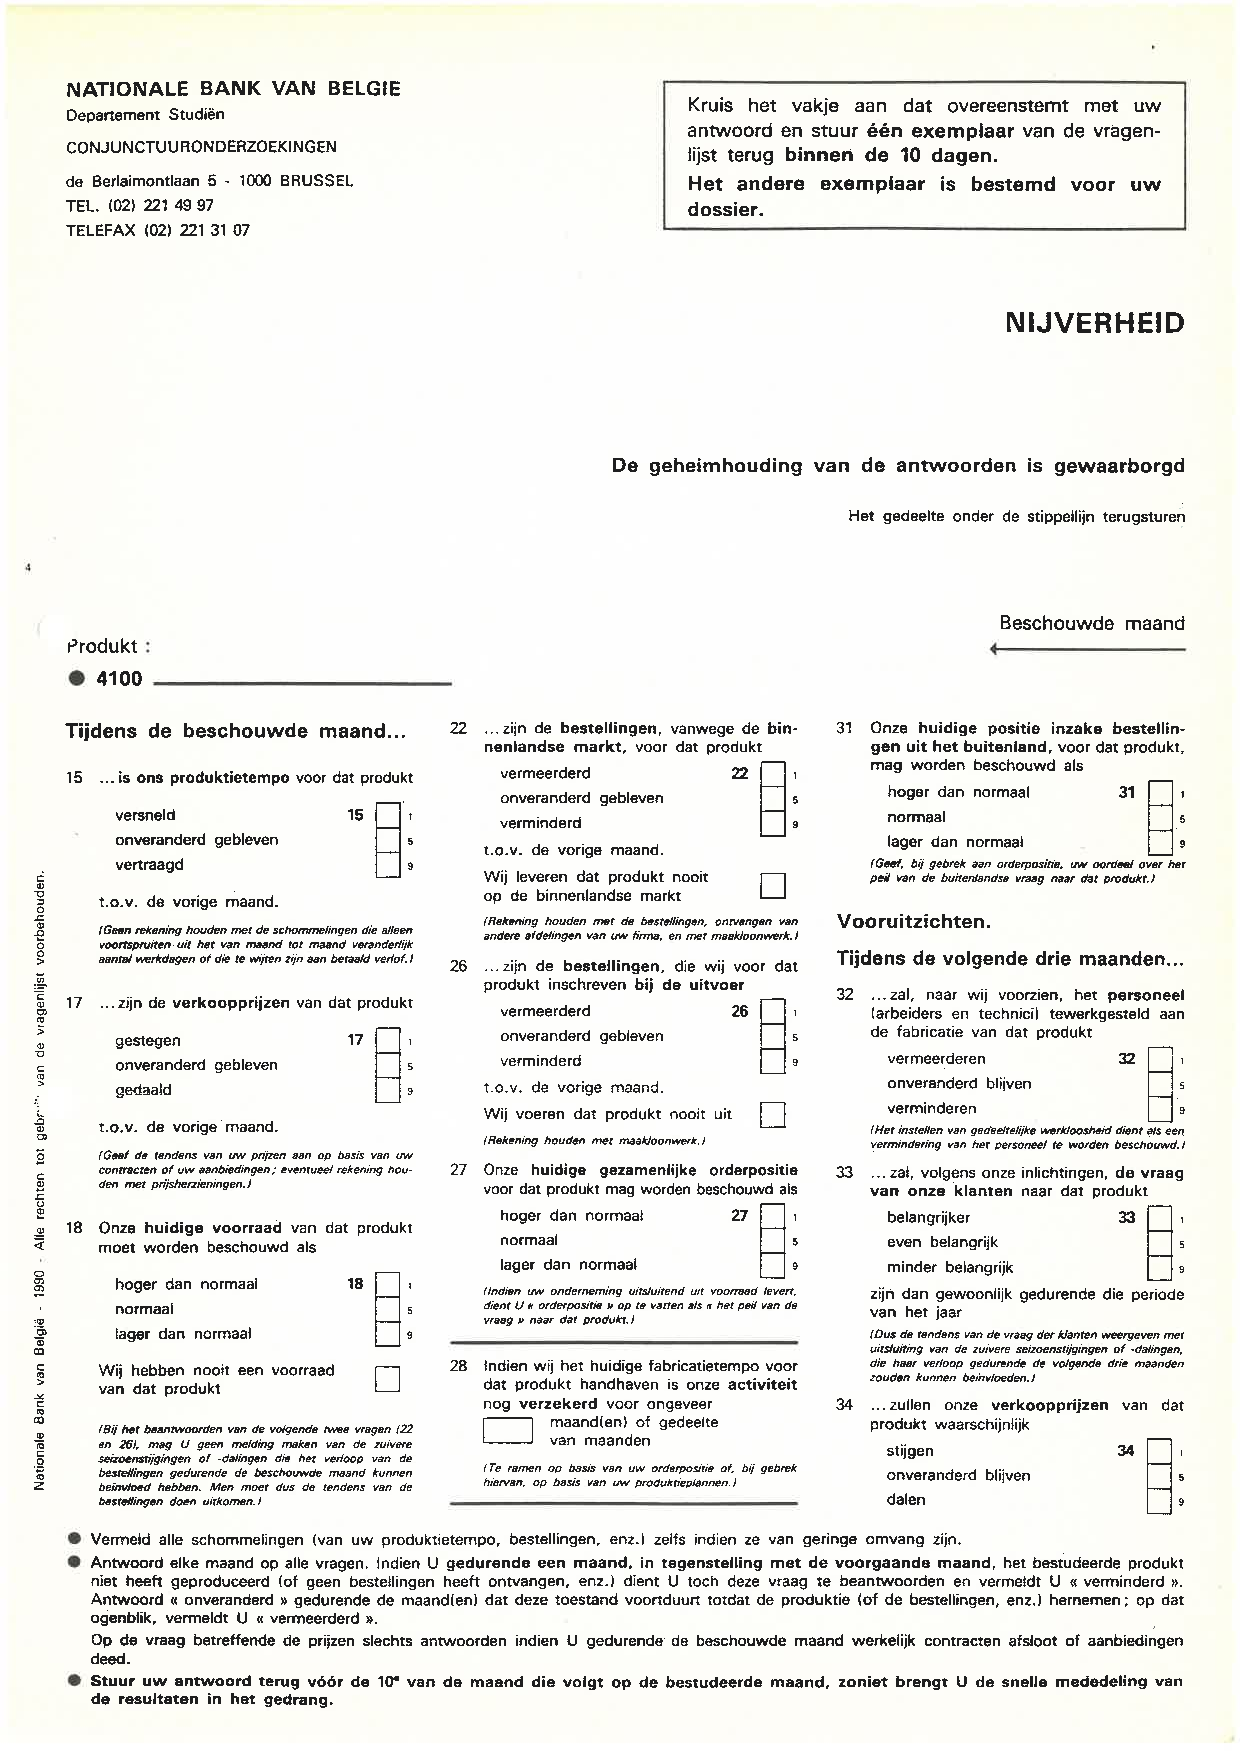
\includegraphics[scale=0.75]{Images/4100N_v1990.pdf}
    \caption{The Business Survey Questionnaire in Dutch for the Industrial Sector in 1990}
    \label{Questionnaire1990}
\end{figure}



\begin{figure}
\begin{subfigure}{.5\textwidth}
  \centering
  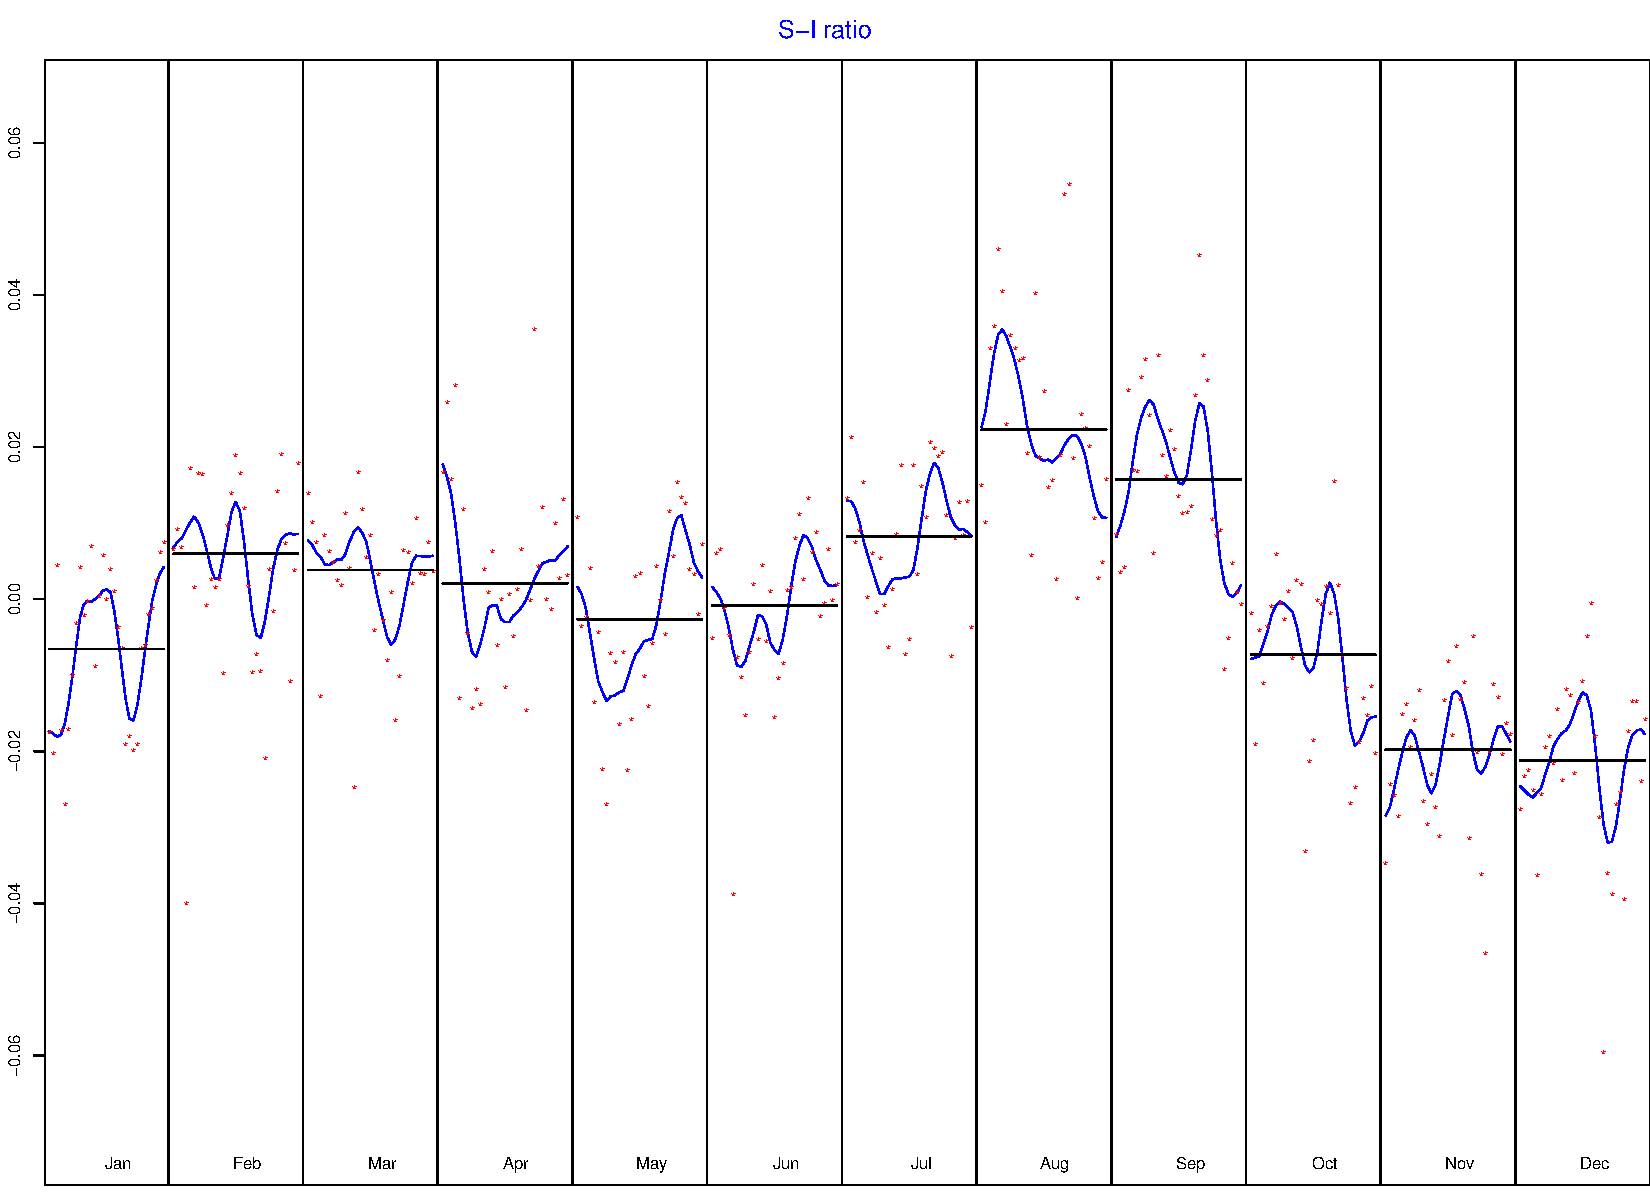
\includegraphics[width=.8\linewidth]{Graphs/S-I_1.pdf}
  \caption{BSI}
\end{subfigure}%
\begin{subfigure}{.5\textwidth}
  \centering
  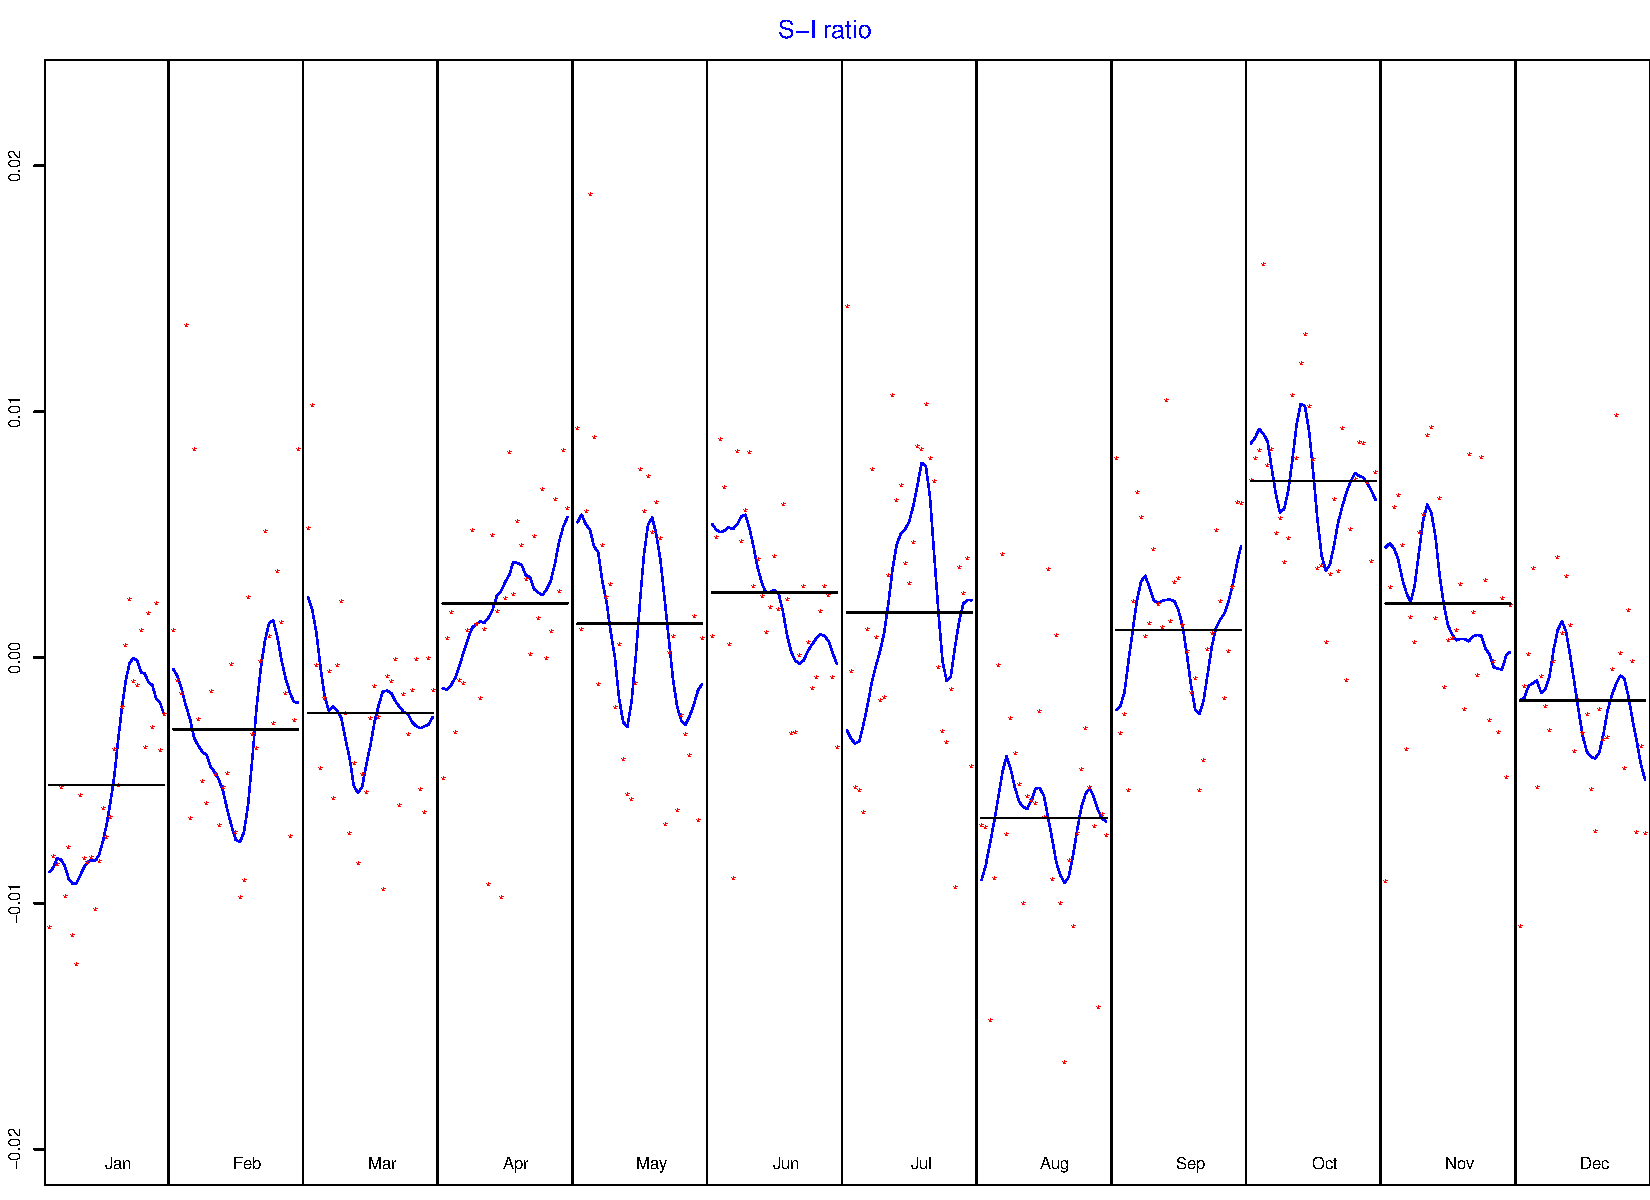
\includegraphics[width=.8\linewidth]{Graphs/S-I_2.pdf}
  \caption{Var(BSI)}
\end{subfigure}
\begin{subfigure}{.5\textwidth}
  \centering
  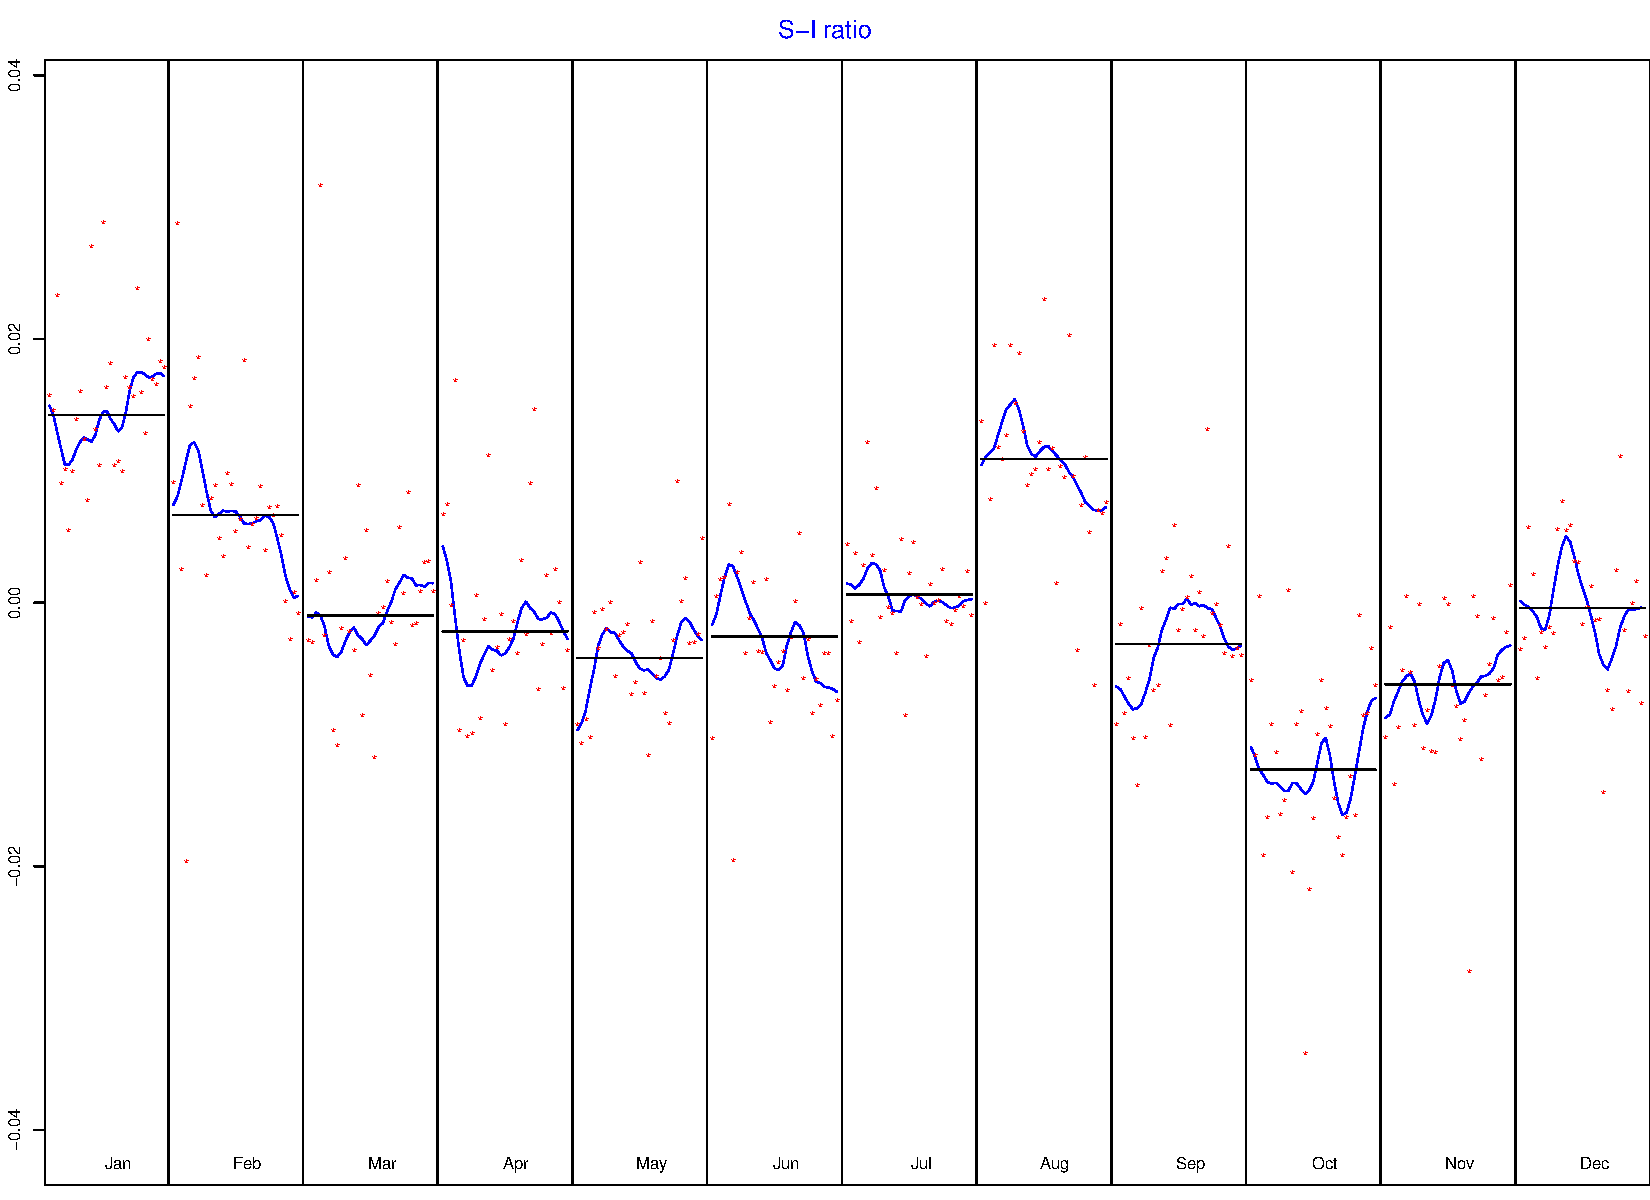
\includegraphics[width=.8\linewidth]{Graphs/S-I_3.pdf}
  \caption{EIR1}
\end{subfigure}
\begin{subfigure}{.5\textwidth}
  \centering
  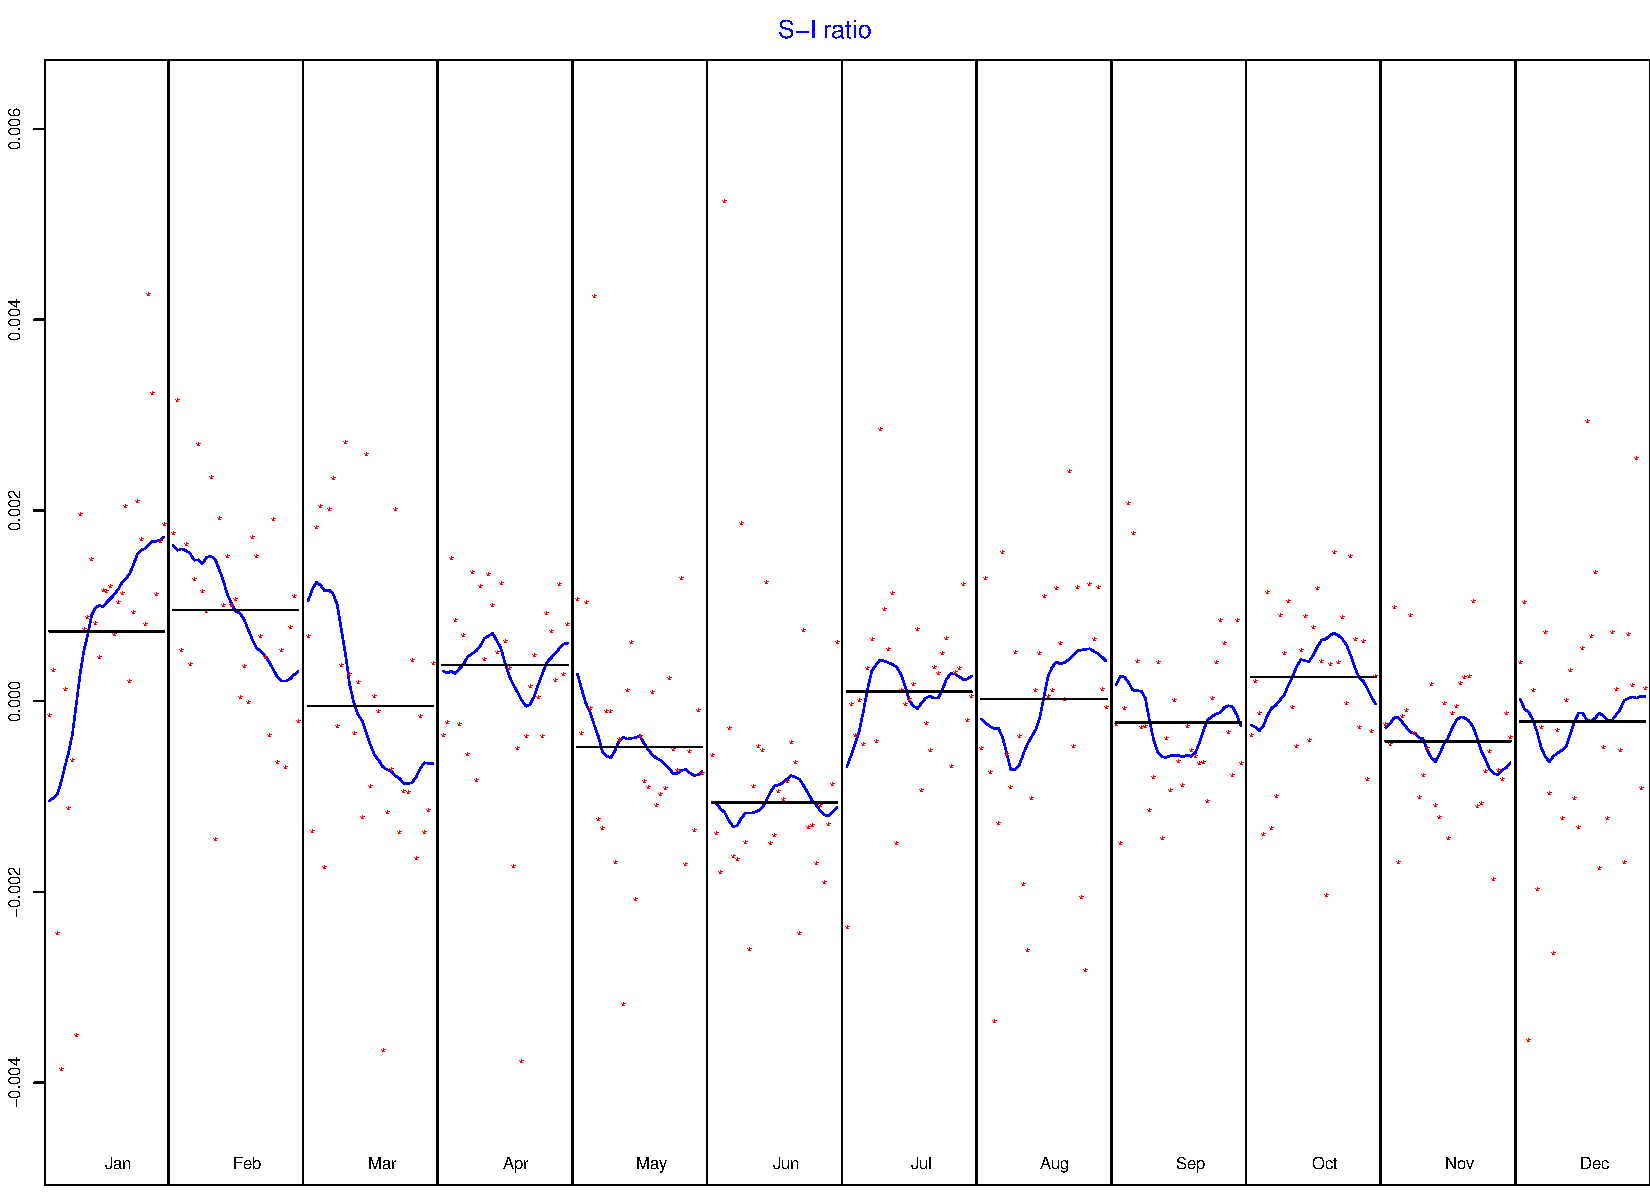
\includegraphics[width=.8\linewidth]{Graphs/S-I_4.pdf}
  \caption{Var(EIR1)}
\end{subfigure}
\begin{subfigure}{.5\textwidth}
  \centering
  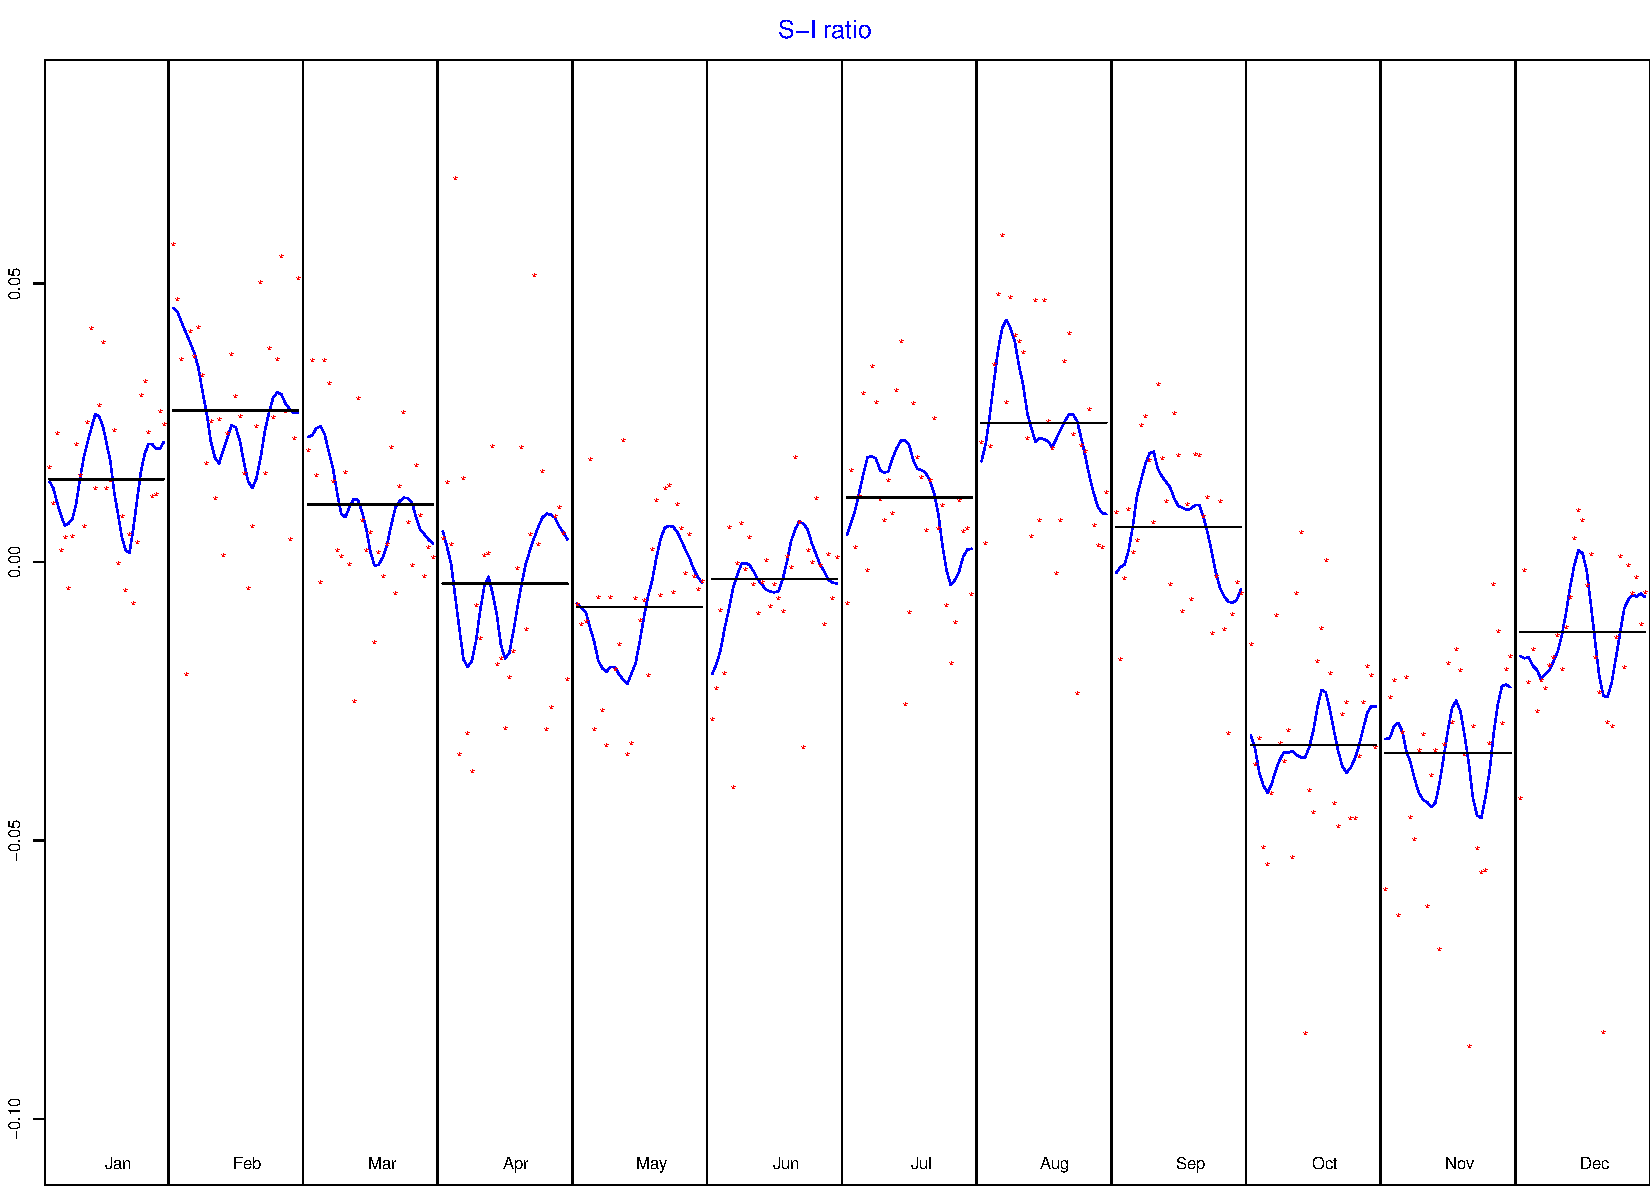
\includegraphics[width=.8\linewidth]{Graphs/S-I_5.pdf}
  \caption{EIR2}
\end{subfigure}
\begin{subfigure}{.5\textwidth}
  \centering
  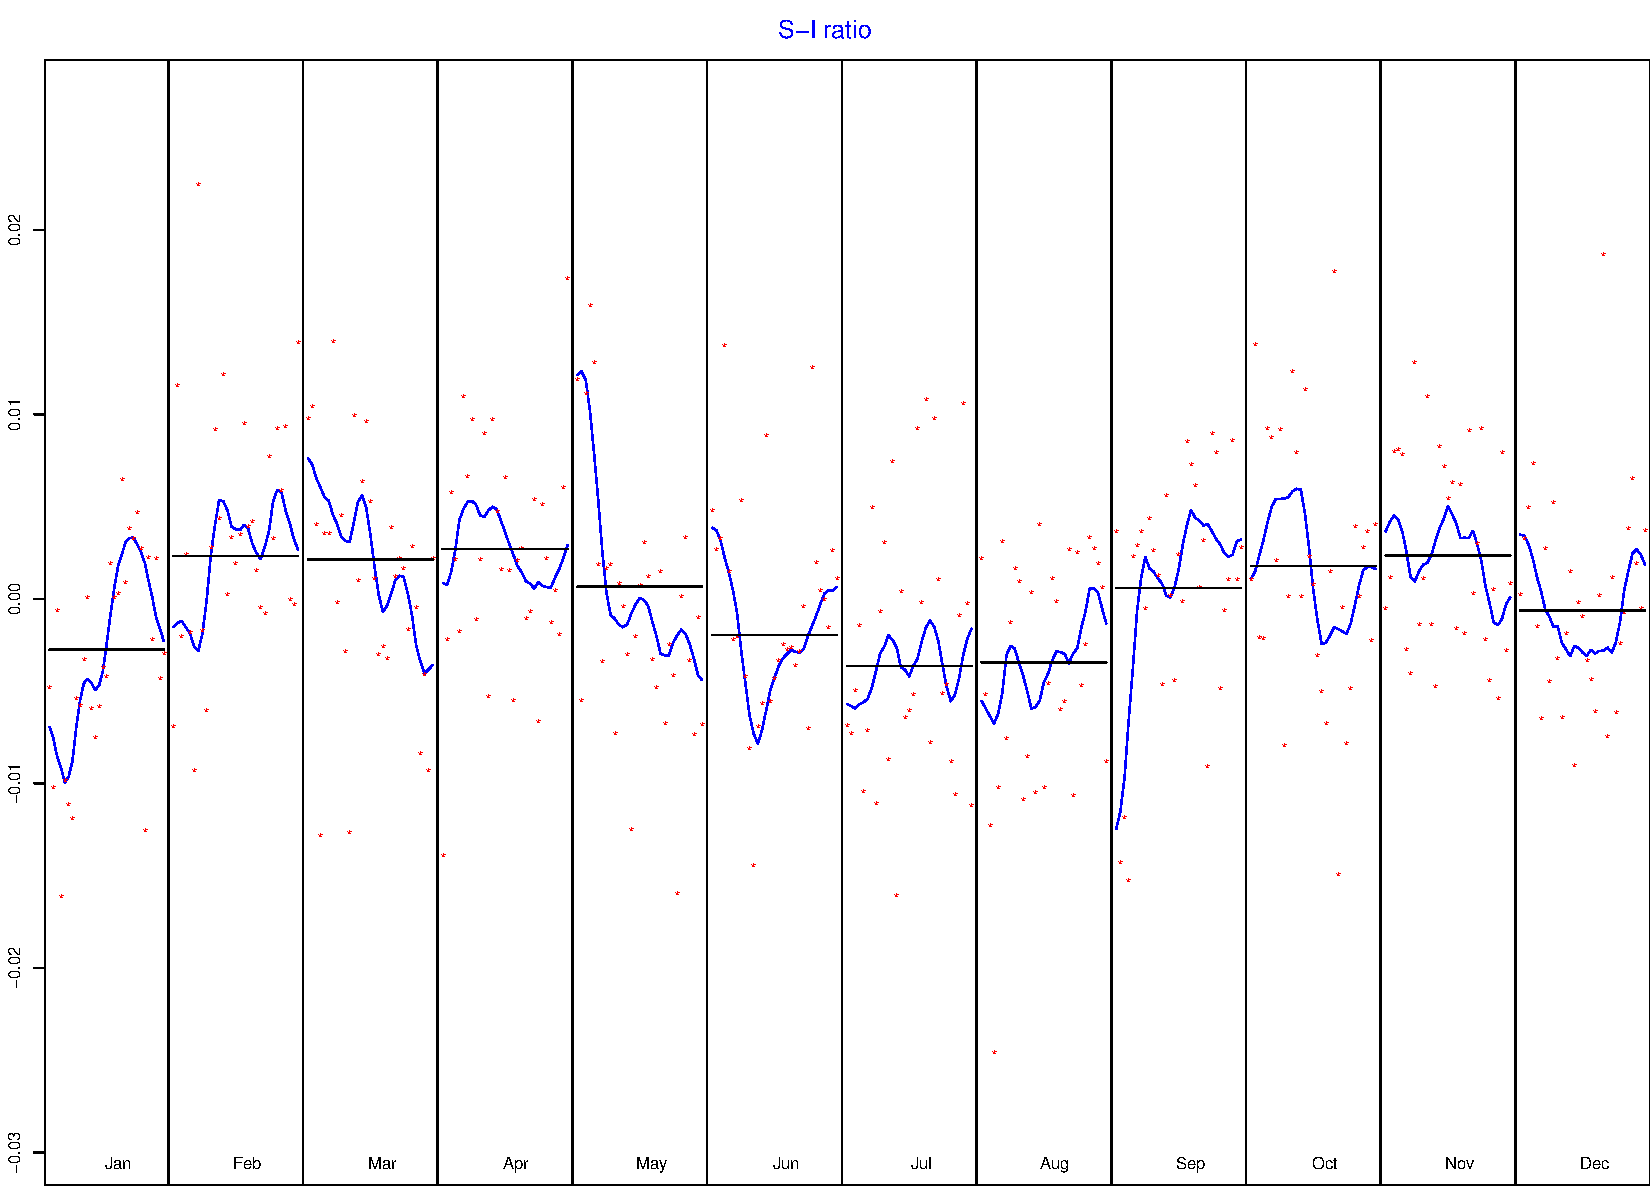
\includegraphics[width=.8\linewidth]{Graphs/S-I_6.pdf}
  \caption{Var(EIR2)}
\end{subfigure}
\begin{subfigure}{.5\textwidth}
  \centering
  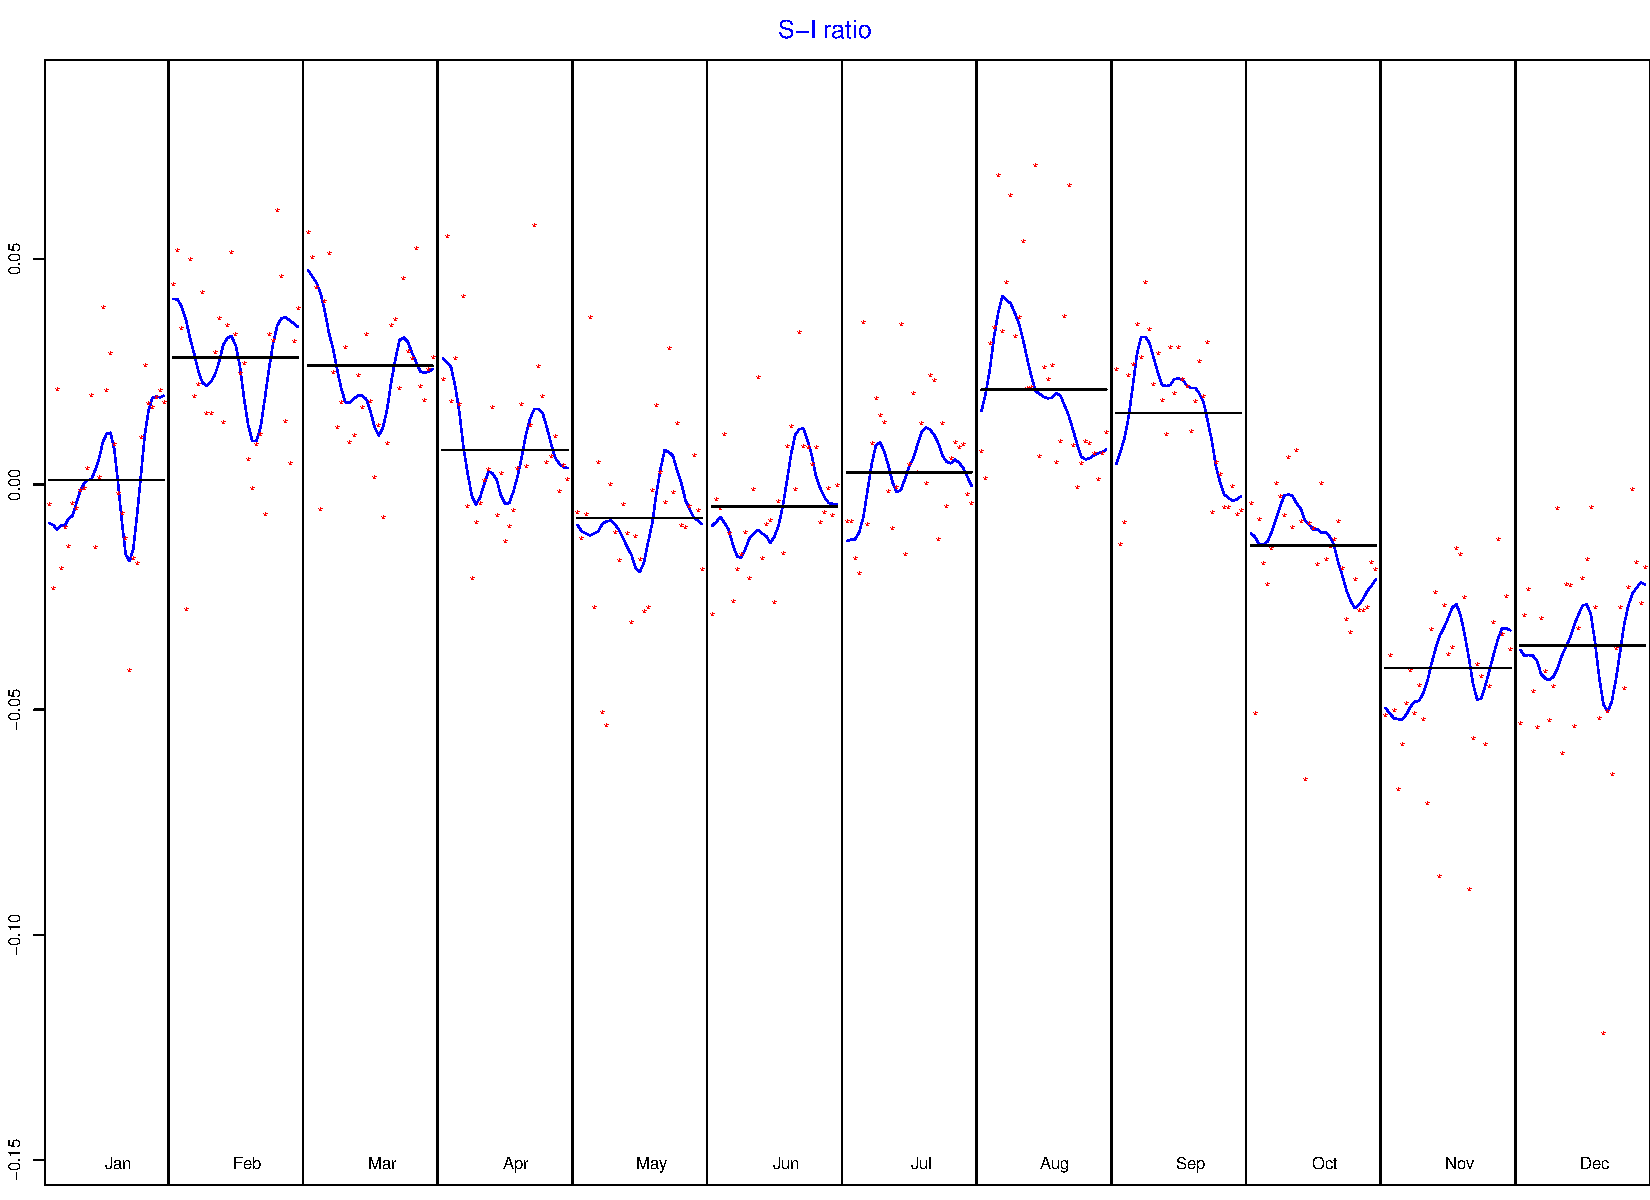
\includegraphics[width=.8\linewidth]{Graphs/S-I_7.pdf}
  \caption{EIR3}
\end{subfigure}
\begin{subfigure}{.5\textwidth}
  \centering
  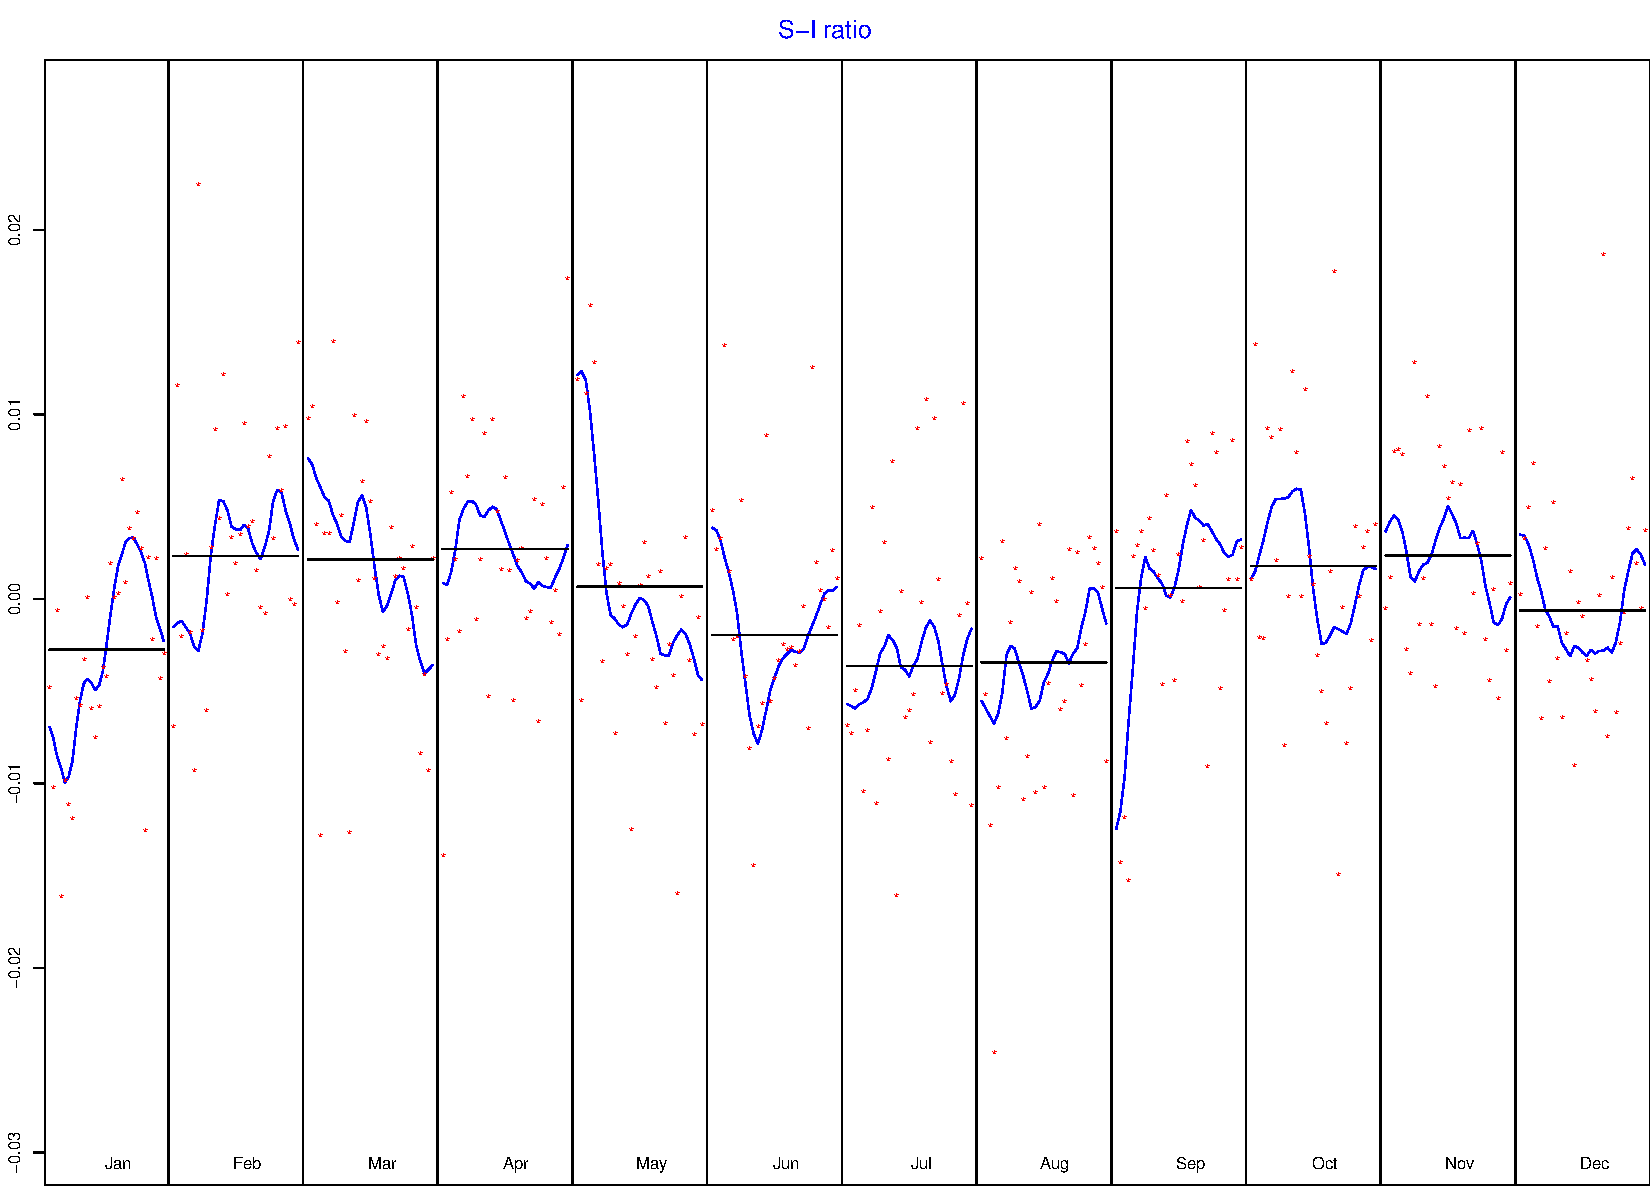
\includegraphics[width=.8\linewidth]{Graphs/S-I_8.pdf}
  \caption{Var(EIR3)}
\end{subfigure}
\caption{S-I plots for the different variables}
\label{fig:S-I seasonal correction RJDemetra}
\end{figure}


\newpage

\begin{table}[H] \centering \footnotesize
  \caption{Linear Regression results for the period 1988 to 2000}
  \label{tab:model comparaison 2000} 
\begin{tabular}{@{\extracolsep{5pt}}lD{.}{.}{-3} D{.}{.}{-3} D{.}{.}{-3} } 
\\[-1.8ex]\hline 
\hline \\[-1.8ex] 
 & \multicolumn{3}{c}{Linear Regression} \\ 
\cline{2-4} 
\\[-1.8ex] & \multicolumn{3}{c}{Year on Year GDP} \\ 
\\[-1.8ex] & \multicolumn{1}{c}{(1)} & \multicolumn{1}{c}{(2)} & \multicolumn{1}{c}{(3)}\\ 
\hline \\[-1.8ex] 
 Constant & 4.437^{***} & 0.660 & -0.519 \\ 
  & (0.211) & (1.899) & (2.041) \\ 
  & & & \\ 
 BSI & 17.374^{***} & 19.212^{***} & 20.327^{***} \\ 
  & (1.547) & (1.758) & (1.813) \\ 
  & & & \\ 
 Var(BSI) &  & 30.545^{*} & 31.371^{**} \\ 
  &  & (15.269) & (14.992) \\ 
  & & & \\ 
 EIR1 &  &  & -37.120^{**} \\ 
  &  &  & (17.899) \\ 
  & & & \\ 
 Var(EIR1) &  &  & 53.535 \\ 
  &  &  & (52.433) \\ 
  & & & \\ 
\hline \\[-1.8ex] 
Observations & \multicolumn{1}{c}{48} & \multicolumn{1}{c}{48} & \multicolumn{1}{c}{48} \\ 
R$^{2}$ & \multicolumn{1}{c}{0.733} & \multicolumn{1}{c}{0.754} & \multicolumn{1}{c}{0.779} \\ 
Adjusted R$^{2}$ & \multicolumn{1}{c}{0.727} & \multicolumn{1}{c}{0.744} & \multicolumn{1}{c}{0.758} \\ 
Residual Std. Error & \multicolumn{1}{c}{0.851} & \multicolumn{1}{c}{0.825} & \multicolumn{1}{c}{0.801} \\ 
AIC & \multicolumn{1}{c}{124.714} & \multicolumn{1}{c}{122.625} & \multicolumn{1}{c}{121.622} \\ 
BIC & \multicolumn{1}{c}{130.327} & \multicolumn{1}{c}{130.109} & \multicolumn{1}{c}{132.849} \\ 
\hline 
\hline \\[-1.8ex] 
\textit{Note:}  & \multicolumn{3}{r}{$^{*}$p$<$0.1; $^{**}$p$<$0.05; $^{***}$p$<$0.01} \\ 
\end{tabular} 
\end{table} 


\begin{figure}[H]
    \centering
    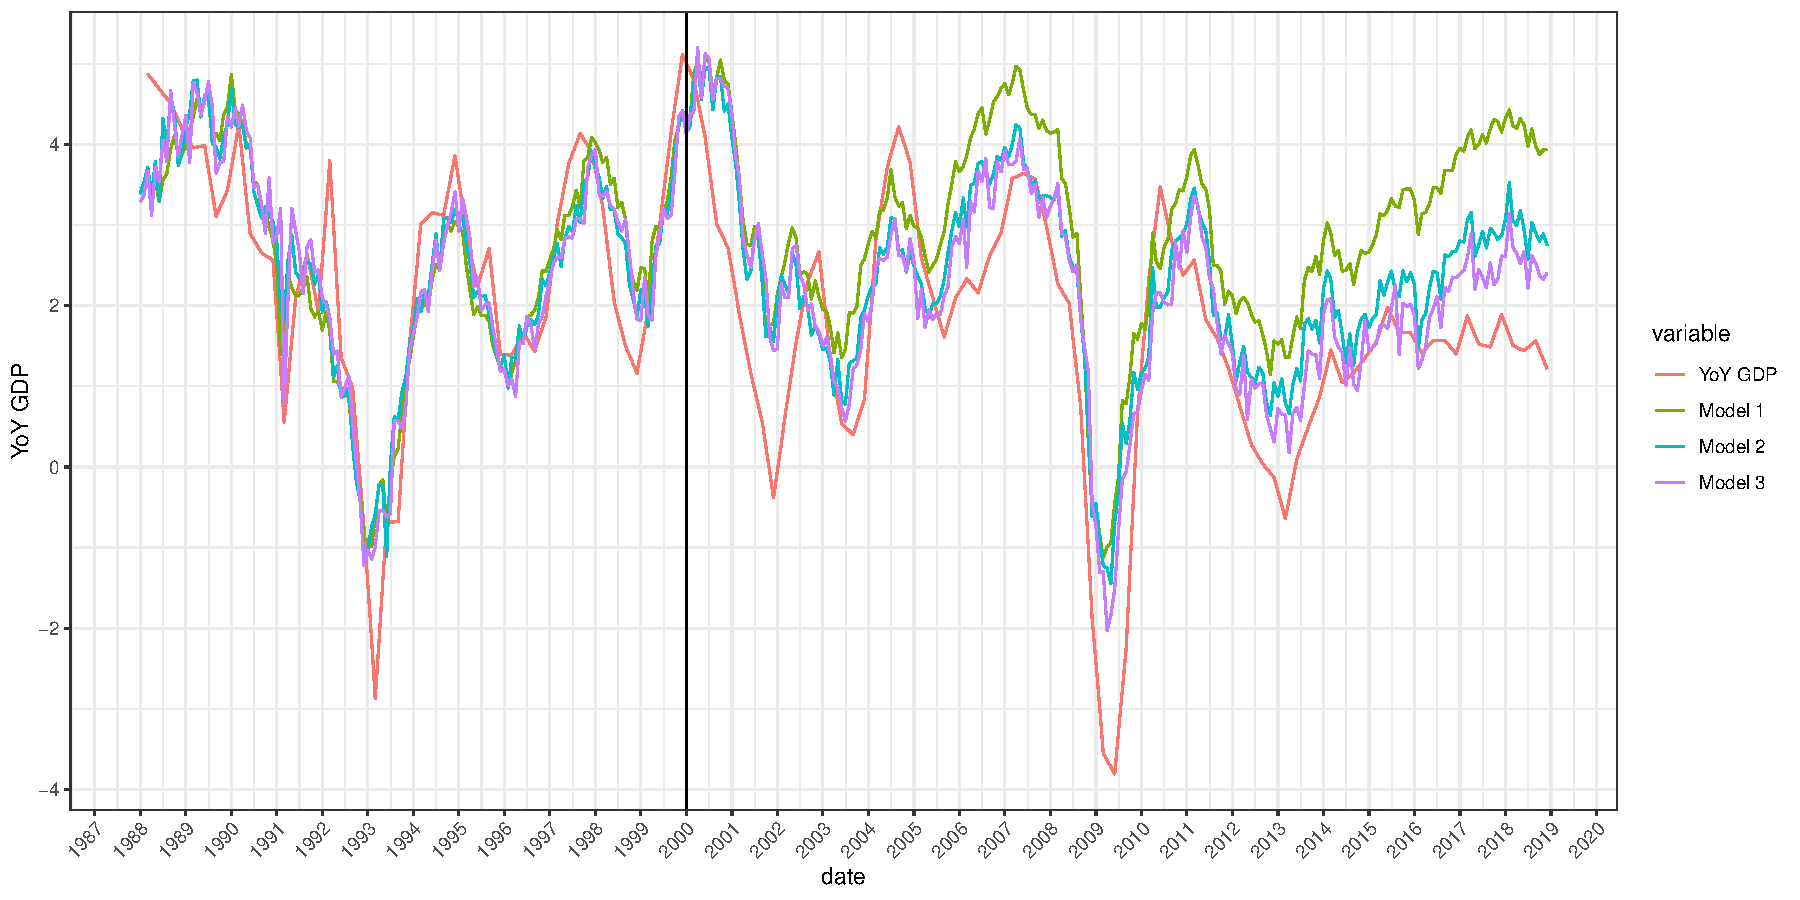
\includegraphics[scale=0.5]{Graphs/predictions2.pdf}
    \caption{Plot of year on year GDP and the different estimation from model 1, 2 and 3 when estimated with the data from 1988 to 2000}
    \label{fig:predictions2}
\end{figure}


\begin{table}[H] \centering \footnotesize
  \caption{Linear Regression results for the period 1988 to 2012}
  \label{tab:model comparaison 2012} 
\begin{tabular}{@{\extracolsep{5pt}}lD{.}{.}{-3} D{.}{.}{-3} D{.}{.}{-3} } 
\\[-1.8ex]\hline 
\hline \\[-1.8ex] 
 & \multicolumn{3}{c}{Linear Regression} \\ 
\cline{2-4} 
\\[-1.8ex] & \multicolumn{3}{c}{Year on Year GDP} \\ 
\\[-1.8ex] & \multicolumn{1}{c}{(1)} & \multicolumn{1}{c}{(2)} & \multicolumn{1}{c}{(3)}\\ 
\hline \\[-1.8ex]
 Constant & 3.871^{***} & -0.686 & -1.349 \\ 
  & (0.171) & (1.054) & (1.102) \\ 
  & & & \\ 
 BSI & 17.243^{***} & 20.939^{***} & 21.499^{***} \\ 
  & (1.341) & (1.491) & (1.478) \\ 
  & & & \\ 
 Var(BSI) &  & 40.466^{***} & 33.997^{***} \\ 
  &  & (9.256) & (10.062) \\ 
  & & & \\ 
 EIR1 &  &  & -33.401^{**} \\ 
  &  &  & (16.292) \\ 
  & & & \\ 
 Var(EIR1) &  &  & 71.077 \\ 
  &  &  & (44.449) \\ 
  & & & \\ 
\hline \\[-1.8ex] 
Observations & \multicolumn{1}{c}{96} & \multicolumn{1}{c}{96} & \multicolumn{1}{c}{96} \\ 
R$^{2}$ & \multicolumn{1}{c}{0.637} & \multicolumn{1}{c}{0.699} & \multicolumn{1}{c}{0.718} \\ 
Adjusted R$^{2}$ & \multicolumn{1}{c}{0.634} & \multicolumn{1}{c}{0.693} & \multicolumn{1}{c}{0.705} \\ 
Residual Std. Error & \multicolumn{1}{c}{1.064} & \multicolumn{1}{c}{0.974} & \multicolumn{1}{c}{0.954} \\ 
AIC & \multicolumn{1}{c}{288.325} & \multicolumn{1}{c}{272.383} & \multicolumn{1}{c}{270.247} \\ 
BIC & \multicolumn{1}{c}{296.018} & \multicolumn{1}{c}{282.641} & \multicolumn{1}{c}{285.633} \\ 
\hline 
\hline \\[-1.8ex] 
\textit{Note:}  & \multicolumn{3}{r}{$^{*}$p$<$0.1; $^{**}$p$<$0.05; $^{***}$p$<$0.01} \\ 
\end{tabular} 
\end{table} 



\begin{figure}[H]
    \centering
    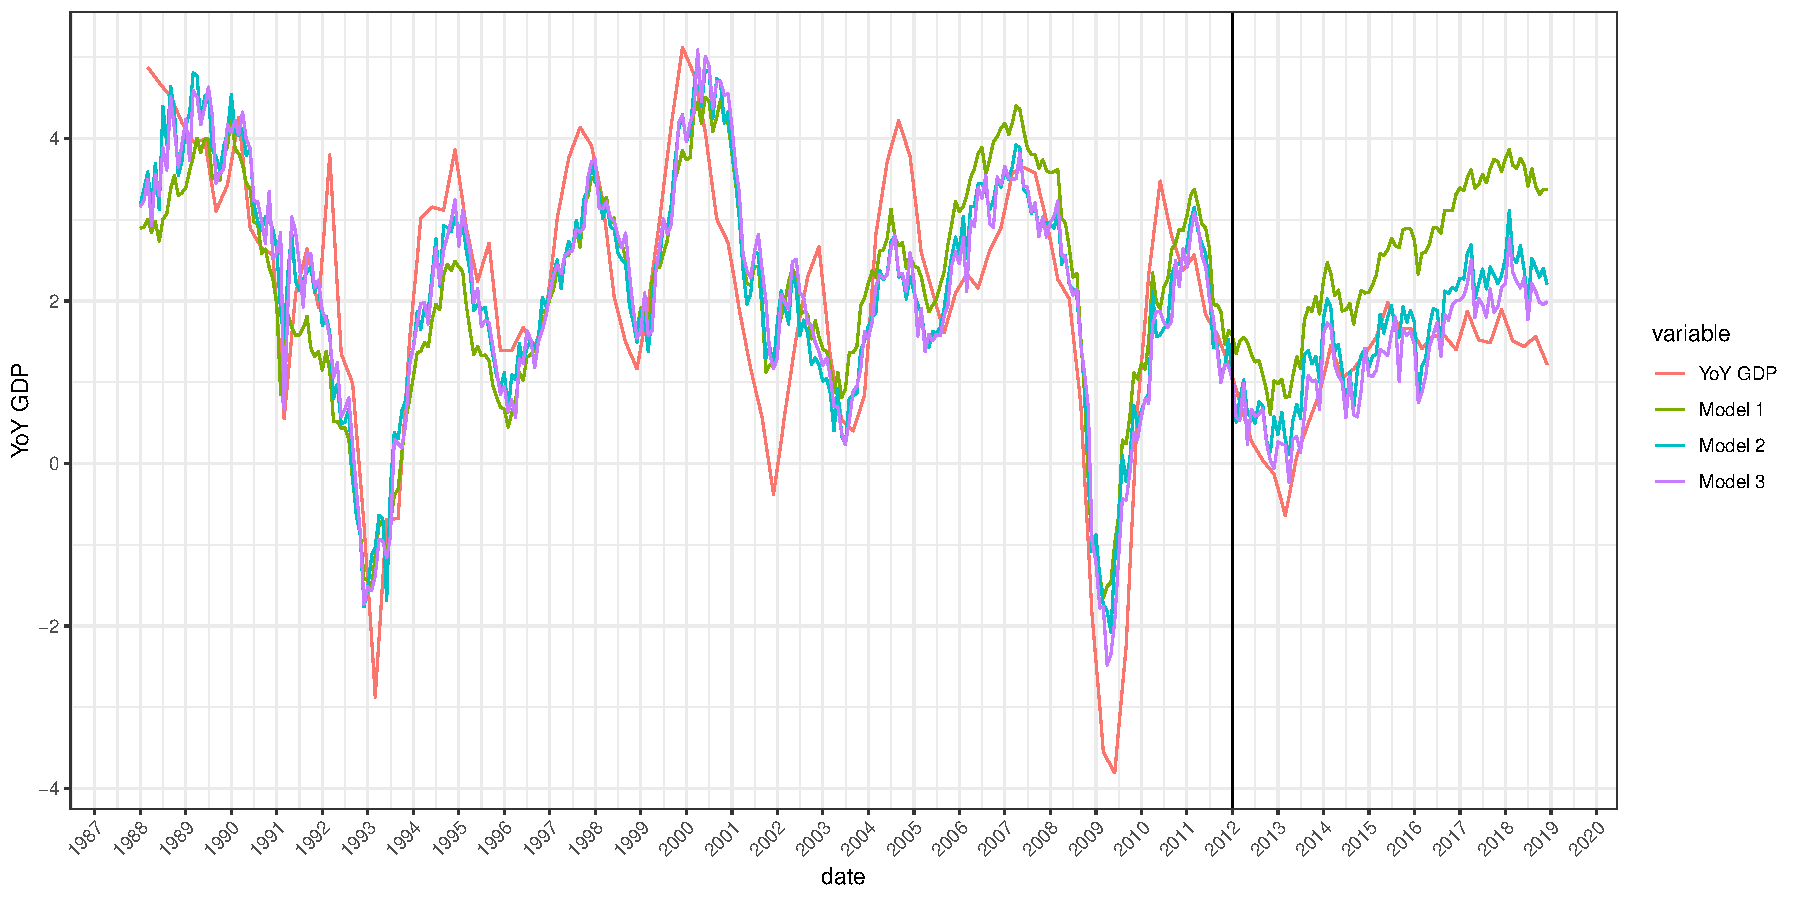
\includegraphics[scale=0.5]{Graphs/predictions3.pdf}
    \caption{Plot of year on year GDP and the different estimation from model 1, 2 and 3 when estimated with the data from 1988 to 2012}
    \label{fig:predictions3}
\end{figure}



\chapter*{Code}
\subsection*{R code for Seasonal Adjustments}

\href{https://github.com/fabricevb/Master-Thesis/blob/master/R Code/Seasonal Correction model data.R}{https://github.com/fabricevb/Master-Thesis/blob/master/R Code/Seasonal Correction model data.R}


\subsection*{R code for Correlation Analysis}

\href{https://github.com/fabricevb/Master-Thesis/blob/master/R Code/Correlations.R}{https://github.com/fabricevb/Master-Thesis/blob/master/R Code/Correlations.R}




\subsection*{R code for Linear Models}

\href{https://github.com/fabricevb/Master-Thesis/blob/master/R Code/Linear Models.R}{https://github.com/fabricevbMaster-Thesis/blob/master/R Code/Linear Models.R}


\newpage

% ----------------------- Back cover ------------------------------
% Please fill in:
% - Department
% - Department's address
% - Telephone number and fax number
% -----------------------------------------------------------------
\thispagestyle{empty}
\sffamily
%
\begin{textblock}{191}(113,-11)
{\color{blueline}\rule{160pt}{5.5pt}}
\end{textblock}
%
\begin{textblock}{191}(168,-11)
{\color{blueline}\rule{5.5pt}{59pt}}
\end{textblock}
%
\begin{textblock}{183}(-24,-11)
\textblockcolour{}
\flushright
\fontsize{7}{7.5}\selectfont
\textbf{Leuven Statistics Research Centre}\\
Celestijnenlaan 200 B Postal box 5307\\
3001 Heverlee, Belgium\\
tel. + 32 16 32 88 75\\
www.lstat.kuleuven.be\\
\end{textblock}
%
\begin{textblock}{191}(154,-7)
\textblockcolour{}
\includegraphics*[height=16.5truemm]{Images/sedes}
\end{textblock}
%
\begin{textblock}{191}(-20,235)
{\color{bluetitle}\rule{544pt}{55pt}}
\end{textblock}



\end{document}